
\chapter{Aircraft with Hose and Drogue}

	The successful implementation of aerial refueling is based on the establishment of accurate docking models, including Aerodynamic Disturbance Models, aircraft model and hose-and-drogue model. Among them, Aerodynamic Disturbance Models have been discussed in detail in the previous chapter, and this chapter will mainly introduce the aircraft model and the hose–and-drogue model during the refueling process. Taking F-16 fighter as an example, its kinematics and dynamics models are analyzed, and the models are decoupled and linearized longitudinally and laterally, which provides convenience for controller design. Secondly, the hose–and-drogue model is established to show the dynamic characteristics of the hose-and-drogue system. Finally, a bow wave effect analysis method based on the hose–and-drogue model is introduced. 

\section{Aircraft Model}

In the process of refueling in the air, the tanker keeps a constant speed and a level flight with fixed height. Because the duration of each docking operation is short, the tanker frame can be regarded as an inertial frame during this period of time, and does not have other dynamic characteristics. In the process of refueling in the air, the receiver must complete various maneuvers to successfully complete the refueling task. Therefore, the receiver model is an important part of the whole air refueling model. This section mainly discusses the building process of the receiver model in detail. First, the nonlinear model of the receiver is established. Then, the nonlinear model is simplified to the horizontal and longitudinal linear model. Finally, the wind field disturbance is added to the model.

\subsection{Nonlinear Mass-varing Model of Receiver Aircraft }
The actual receiver is a complex dynamic system, its mass is time-varying during flight, and its structure also has the characteristics of elastic deformation. In addition, the rotation of the Earth causes the vehicle to be subject to centrifugal and Gothic acceleration, while the gravitational acceleration also varies with altitude. Therefore, it is not realistic to establish a completely accurate aircraft model, and it is of practical significance to simplify the aircraft model and flight environment appropriately. Before establishing the motion equation of the receiver, the following assumptions are proposed:

\begin{enumerate}
	\item 	Ignoring the curvature of the earth, the "flat earth hypothesis" is adopted, and the ground coordinate system is assumed to be an inertial coordinate system. In this case, the tanker maintains uniform speed and flies in a straight line, so the tanker coordinate system is also an inertial coordinate system.
	
	\item The receiver system includes the aircraft mechanical body part and the fuel tank part. The body part of the receiver is a rigid body with constant mass, regardless of the elastic deformation of the fuselage and wing during flight, and the origin of the body coordinate system is located at the mass center of the body part of the receiver. The change of the fuel part of the fuel tank causes the change of the total mass and moment of inertia of the receiver.
	
	\item The mechanical body of the receiver system is assumed to be rigid and symmetric about the $o_{\rm{r}}x_{\rm{r}}z_{\rm{r}}$ plane of the body coordinate system, with both external shape and internal mass symmetry. This assumption is applicable to most aircraft. The advantage of this assumption is that the modeling of the mechanical body of the aerial refueling system can directly use traditional constant mass aircraft modeling methods, and the existing aerodynamic parameters can be directly applied to the modeling process of mass-varing aircraft.
	
	\item Ignoring the fuel mass in the fuel transfer pipe and fuel consumption during normal flight. In other words, the receiver system only experiences a mass change during the refueling phase, while in other phases it is considered as a rigid body with constant mass. The mass-varing model is used only during the refueling phase, while in other phases, the receiver system model remains the same as that of a traditional constant mass aircraft.
	
	\item The receiver system has $k$ fuel tanks, and the positions of the fuel tanks and the distribution of fuel mass are symmetric. Each fuel tank is considered as a variable mass block, where the mass of fuel in the $j$th fuel tank is ${m_j},j \in \left\{ {1,2,...,k} \right\}$, and the position vector $\mathbf{r}_{j}$ from the center of mass ${o_j}$ to the origin ${o_{\rm{r}}}$ of the aerial refueling system's body coordinate system is constant.
\end{enumerate}

Based on the above assumptions, the six-degrees-of-freedom motion equations of the variable mass receiver system can be established. Fig. \ref{fig4.1} shows a diagram of an F-16 receiver. The dynamics of the receiver can be described by the variations of position, velocity, attitude angles, and angular velocity with respect to time. In the process of establishing the nonlinear model for the variable mass receiver system, for simplicity, the following notations for the variables are used:
$\mathbf{p}\rm{_{r}^{g} }\triangleq \left[ {\begin{array}{*{20}{c}}
	x_\mathrm{r}&y_\mathrm{r}&h_\mathrm{r}
	\end{array}} \right]^{\rm{T}}$ represents the position of the receiver system in the Earth coordinate system;
$\mathbf{v}\mathrm{_{r}^{b}} \triangleq \left[ {\begin{array}{*{20}{c}}
	u_\mathrm{r}&v_\mathrm{r}&w_\mathrm{r}
	\end{array}} \right]^{\rm{T}}$ represents the velocity vector of the receiver system in the body coordinate system, where $u$ is the longitudinal velocity magnitude, $v$ is the lateral velocity magnitude, and $w$ is the normal velocity magnitude;
$\bm{\Theta} _\mathrm{r} \triangleq \left[ {\begin{array}{*{20}{c}}
	\phi &\theta &\psi 
	\end{array}} \right]^{\rm{T}}$ represents the attitude angles of the receiver system;
$\boldsymbol{\omega} \mathrm{_{r}^{b}} \triangleq \left[ {\begin{array}{*{20}{c}}
	p&q&r
	\end{array}} \right]^{\rm{T}}$ represents the body angular velocity of receiver system;
$\bf{u}_\mathrm{r} \triangleq \left[ {\begin{array}{*{20}{c}}
	\delta _{t}&\delta _{e}&\delta _{a}&\delta _{r}
	\end{array}} \right]^{\rm{T}}$ represents the control inputs of the receiver system, including the engine input, elevator deflection angle, aileron deflection angle, and rudder deflection angle. It is also defined that a downward deflection of the elevator angle $\delta _{e}$ is considered positive, a leftward deflection of the rudder angle $\delta _{r}$ is considered positive, and an upward deflection of the left aileron and a downward deflection of the right aileron are considered positive.

According to Newton's second law, the linear equations of motion for the receiver under external forces in an inertial reference frame are as follows 
\begin{equation}\label{eq4.1}
\mathbf{F} = \frac{\text{d}}{{\text{d}t}}\left( {m\mathbf{v}\mathrm{_{r}^{g}}} \right)
\end{equation}
where $\mathbf{F}$ represents the total external force acting on the receiver, including aerodynamic forces, engine thrust, and gravity; $\mathbf{v}\mathrm{_r^g}$ represents the velocity vector of the center of mass of the receiver system in the Earth coordinate system; $m$ represents the total mass of the receiver system, satisfying the following equation 
\begin{equation}\label{eq4.2}
m = {m_0} + {m_f} .
\end{equation}
Here, ${m_0}$ is a constant representing the mass of the mechanical body of the aircraft; ${m_f}$ is a variable representing the mass of the fuel in the fuel tank, satisfying the following equation 
\begin{equation}\label{eq4.3}
{m_f} = \sum\limits_{j = 1}^k {{m_j}} .
\end{equation}
It can be deduced from Eq. (\ref{eq4.2}) and Eq. (\ref{eq4.3}) that
\begin{equation}\label{eq4.4}
\dot m = {\dot m_0} + {\dot m_f} = {\dot m_f} = \sum\limits_{j = 1}^k {{{\dot m}_j}} .
\end{equation}
Therefore, the mass change of the receiver is entirely determined by the fuel mass change in the fuel tank of the receiver.

The equation of angular motion for the receiver under the influence of external torque is as follows
\begin{equation}\label{eq4.5}
\mathbf{M} = \frac{\mathrm{d}\mathbf{L}\mathrm{_r^g}}{\mathrm{d}t}
\end{equation}
where $\mathbf{L}\mathrm{_r^g}$ is the angular momentum, $\mathbf{M}$ is the total external torque acting on the receiver, including aerodynamic torque and the torque generated by the gravitational force of the fuel on the aircraft’s mechanical center of gravity, as the center of gravity of the fuel in each fuel tank does not coincide with the aircraft’s mechanical center of gravity.
\begin{figure}[th]
	\centering
	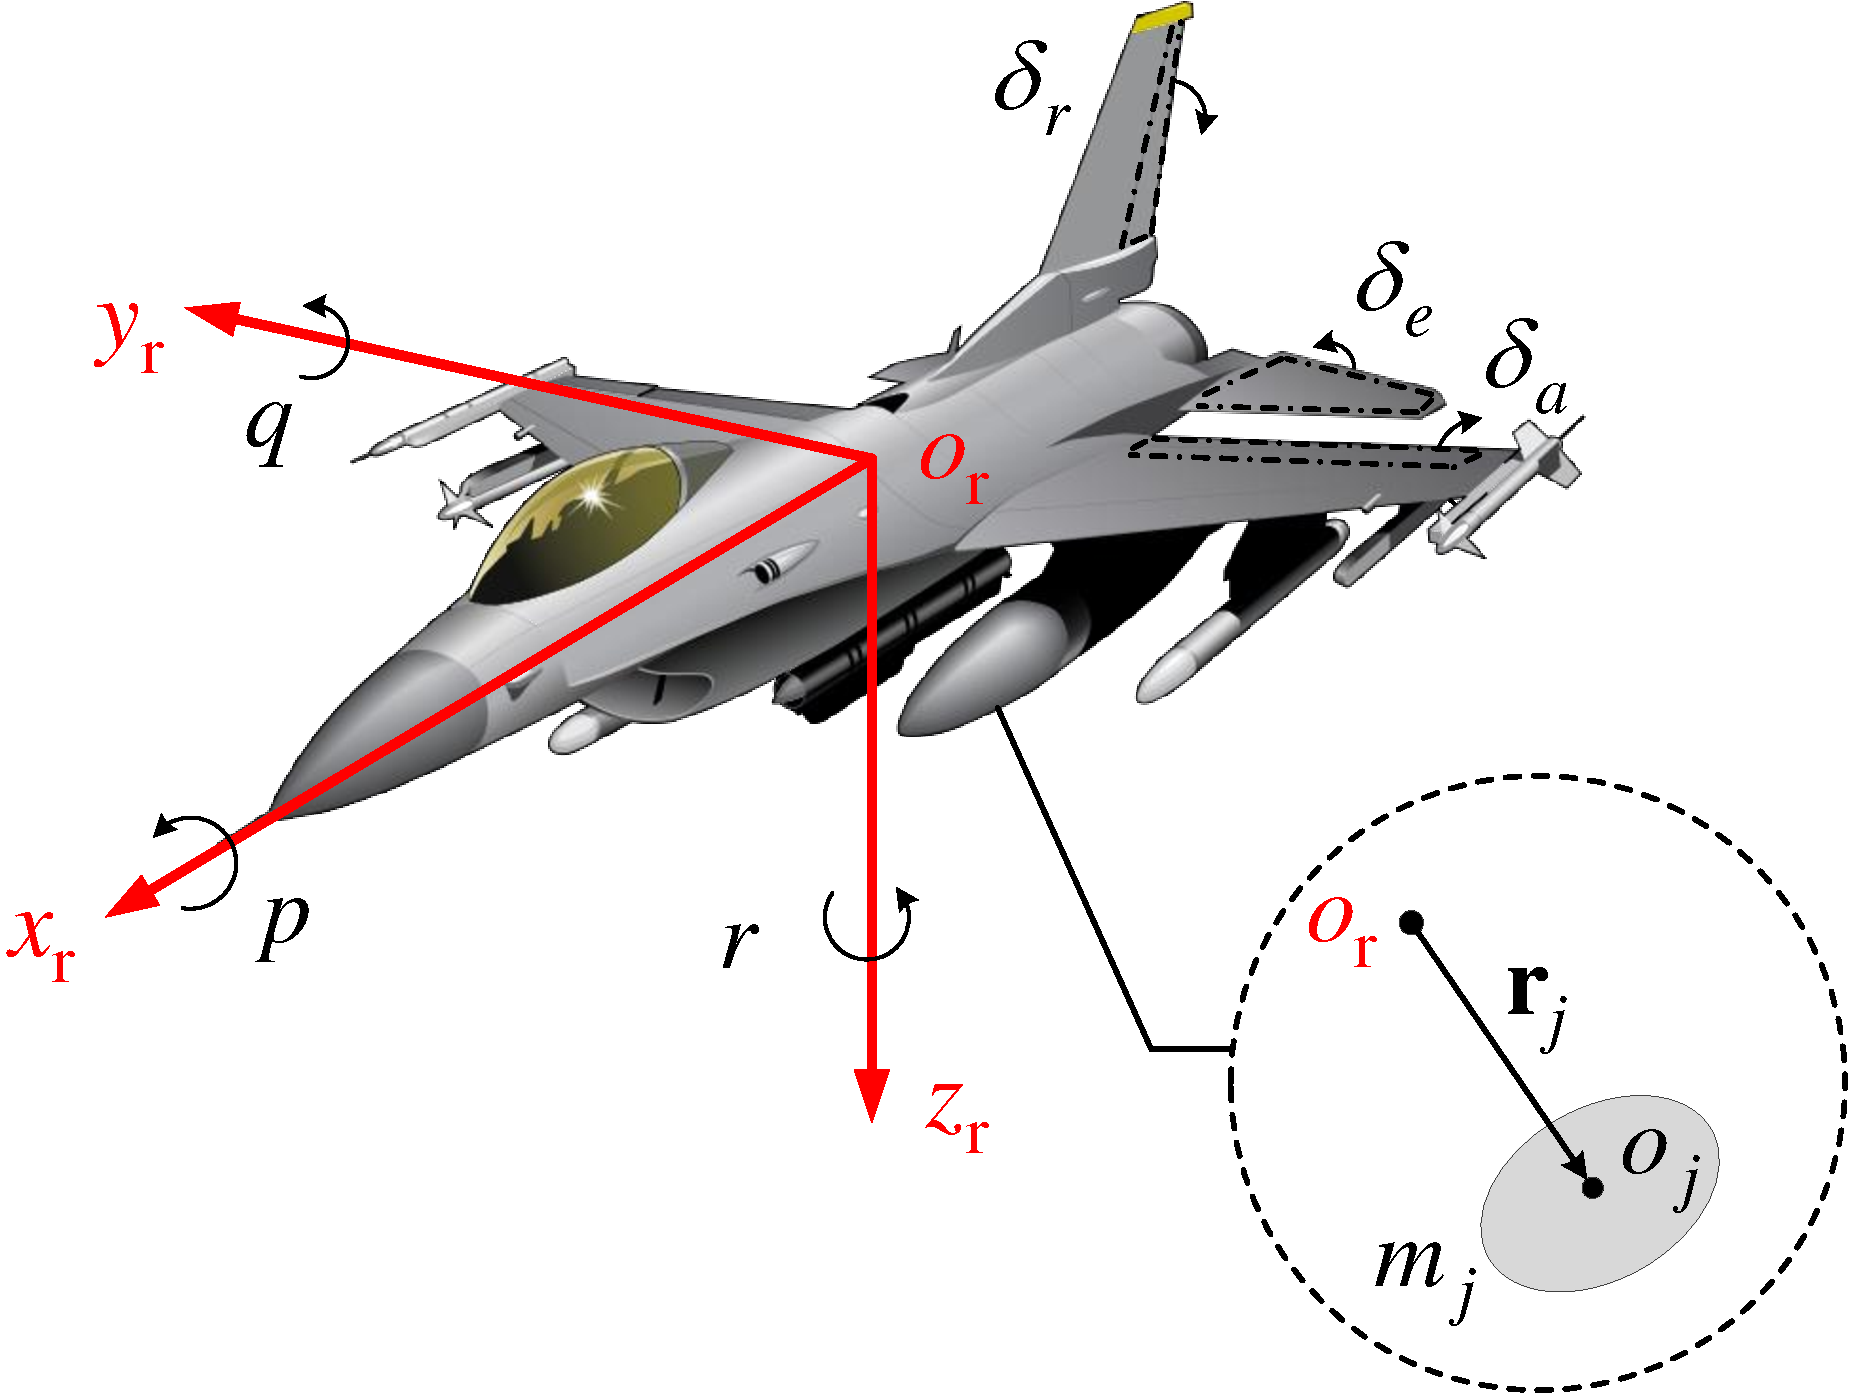
\includegraphics[width=0.5\textwidth]{Figures/Figs_Ch3/fig1.pdf}
	\caption{Schematic diagram of the F-16 refueling receiver}\label{fig4.1}
\end{figure}

\begin{itemize}	
	\item  
	Force Equations:
\end{itemize}


First, consider Eq. (\ref{eq4.1}). In order to establish the motion relationship of the receiver relative to the ground coordinate system, the velocity ${\mathbf{v}_{\rm{r}}}$ of the receiver is decomposed in the body coordinate system. In the body coordinate system, Eq. (\ref{eq4.1}) can be expressed as 
\begin{equation}\label{eq4.6}
\mathbf{F}^{\mathrm{b}}=\frac{\mathrm{d}}{\mathrm{d} t}\left(m \mathbf {v}_{\mathrm{r}}^{\mathrm{b}}\right)+\bm{\omega}_{\mathrm{r}}^{\mathrm{b}} \times m \mathbf{v}_{\mathrm{r}}^{\mathrm{b}}
\end{equation}
where $\mathbf{v}\mathrm{_r^b}$ is the velocity vector of the receiver’s center of gravity in the body coordinate system, and $\bm{\omega}\mathrm{_r^b}$ is the total angular velocity vector of the receiver relative to the ground coordinate system.

In the receiver body coordinate system, $\mathbf{v}\mathrm{_r^b}$ and $\bm{\omega}\mathrm{_r^b}$ can be decomposed into
\begin{equation}\label{eq4.7}
\mathbf{v}\mathrm{_r^b} = \mathbf{i}\mathrm{^b}u\mathrm{_r} + \mathbf{j}\mathrm{^b}v\mathrm{_r} + \mathbf{k}\mathrm{^b}w\mathrm{_r}
\end{equation}
\begin{equation}\label{eq4.8}
\bm{\omega}\mathrm{_r^b} = \mathbf{i}\mathrm{^b}p + \mathbf{j}\mathrm{^b}q + \mathbf{k}\mathrm{^b}r
\end{equation}
where $\mathbf{i}\mathrm{^b},\mathbf{j}\mathrm{^b}$ and $\mathbf{k}\mathrm{^b}$are the unit vectors of the $o\mathrm{_r}x\mathrm{_r}$-axis, $o\mathrm{_r}y\mathrm{_r}$-axis, and $o\mathrm{_r}z\mathrm{_r}$-axis of the receiver body coordinate system.

Therefore, the first term of Eq. (\ref{eq4.6}) can be expressed as
\begin{equation}\label{eq4.9}
\frac{\mathrm{d}}{\mathrm{d}t}\left( m\mathbf{v}\mathrm{_r^b} \right) = \dot{ m}\mathbf{v}\mathrm{_r^b} + m\dot{\mathbf{v}}\mathrm{_r^b} = \mathbf{i}\mathrm{^b}\left( {\dot mu\mathrm{_r} + m\dot{u}\mathrm{_r}} \right) + \mathbf{j}\mathrm{^b}\left( \dot mv\mathrm{_r} + m\dot{z}\mathrm{_r} \right) + \mathbf{k}\mathrm{^b}\left( \dot mw\mathrm{_r}+ m{\dot w}\mathrm{_r} \right)
\end{equation}
where $\dot{ m}$ is given by Eq. (\ref{eq4.4}). The second term of Eq. (\ref{eq4.6}) can be expressed as
\begin{equation}\label{eq4.10}
\bm{\omega}\mathrm{_r^b} \times m\mathbf{v}\mathrm{_r^b} = m\left| {\begin{array}{*{20}{c}}
	\mathbf{i}\mathrm{^b}&\mathbf{j}\mathrm{^b}&\mathbf{k}\mathrm{^b}\\
	p&q&r\\
	u\mathrm{_r}&v\mathrm{_r}&w\mathrm{_r}
	\end{array}} \right| = \mathbf{i}\mathrm{^b}m\left( w\mathrm{_r}q - v\mathrm{_r}r \right) + \mathbf{j}\mathrm{^b}m\left( u\mathrm{_r}r - w\mathrm{_r}p\right) + \mathbf{k}\mathrm{^b}m\left( v\mathrm{_r}p - u\mathrm{_r}q \right).
\end{equation}

%Decompose the external force $\mathbf{F}$ into body coordinate system
Represent $\mathbf{F}$ in the form of components in the body coordinate system as
\begin{equation}\label{eq4.11}
\mathbf{F}\mathrm{^b} = \mathbf{i}\mathrm{^b}F_{x}^\mathrm{b} + \mathbf{j}\mathrm{^b}F_y^\mathrm{b} + \mathbf{k}\mathrm{^b}F_z^\mathrm{b}.
\end{equation}
Therefore, substituting Eqs. (\ref{eq4.9}), (\ref{eq4.10}), and (\ref{eq4.11}) into Eq. (\ref{eq4.6}), one can obtain
\begin{equation}\label{eq4.12}
\begin{array}{l}
F_x^\mathrm{b} = m\left( \dot u\mathrm{_r} + w\mathrm{_r}q - v\mathrm{_r}r \right) + \dot mu\mathrm{_r}\\
F_y^\mathrm{b} = m\left( \dot v\mathrm{_r} + u\mathrm{_r}r - w\mathrm{_r}p \right) + \dot mv\mathrm{_r}\\
F_z^\mathrm{b} = m\left( \dot w\mathrm{_r} + v\mathrm{_r}p - u\mathrm{_r}q \right) + \dot mw\mathrm{_r} .
\end{array} 
\end{equation}
The total external force $\mathbf{F}$ includes gravity, aerodynamic force, and engine thrust. Assuming the engine thrust is $F_{T}$ and its direction is along the ${o_\mathrm{_r}}{x_\mathrm{_r}}$-axis of the body coordinate system. In the body coordinate system, the component of gravity is represented as follows
\begin{equation}\label{eq4.13}
\left[ \begin{array}{l}
G_x^\mathrm{b}\\
G_y^\mathrm{b}\\
G_z^\mathrm{b}
\end{array} \right] = \left[ \begin{array}{c}
- mg\sin \theta \\
mg\cos \theta \sin \phi \\
mg\cos \theta \cos \phi 
\end{array} \right]
\end{equation}
where $g$ is the gravitational acceleration. The aerodynamic force components along the three axes of the body coordinate system are denoted as $\bar{ X}, \bar{ Y}$ and $\bar{ Z}$, and their magnitudes are related to the receiver's airspeed ${V_\mathrm{r}}$, air density $\rho $, wing area $S$, wingspan $b$, angle of attack $\alpha $, sideslip angle $\beta $, and control surface deflection angle $	\boldsymbol{\delta}=[  {\delta}_{\rm{a}}  ,    {\delta}_{\rm{r}}   , {\delta}_{\rm{e}}  ,   {\delta}_{\rm{t}}  ]$, etc. The aerodynamic force components can be represented as follows
\begin{equation}\label{eq4.14}
\begin{array}{l}
\bar X = \bar qS{C_{{X_T}}}\left( {\alpha ,\beta ,p,q,r,\boldsymbol{\delta} ,...} \right)\\
\bar Y = \bar qS{C_{{Y_T}}}\left( {\alpha ,\beta ,p,q,r,\boldsymbol{\delta} ,...} \right)\\
\bar Z = \bar qS{C_{{Z_T}}}\left( {\alpha ,\beta ,p,q,r,\boldsymbol{\delta} ,...} \right)
\end{array}
\end{equation}
where $\bar q = 0.5\rho V_\mathrm{r}^2$ represents dynamic pressure, $S$ is the wing area, and the aerodynamic coefficients ${C_{{X_T}}},{C_{{Y_T}}}$ and ${C_{{Z_T}}}$ can be obtained from wind tunnel data or flight data. Interested readers can refer to reference \cite{nguyen_simulator_1979} for the specific forms of the aerodynamic coefficients.

Thus, the force equations for the receiver in the body coordinate system can be represented as follows
\begin{equation}\label{eq4.15}
\begin{array}{l}
{{\dot u}\mathrm{_r}} = r{v\mathrm{_r}} - q{w\mathrm{_r}} - g\sin \theta  + \frac{1}{m}\left( {\bar X + {F_T}} \right) - \frac{{\dot m{u\mathrm{_r}}}}{m}\\
{{\dot v}\mathrm{_r}} = p{w\mathrm{_r}} - r{u\mathrm{_r}} + g\sin \phi \cos \theta  + \frac{1}{m}\bar Y - \frac{{\dot m{v\mathrm{_r}}}}{m}\\
{{\dot w}\mathrm{_r}} = q{u\mathrm{_r}} - p{v\mathrm{_r}} + g\cos \phi \cos \theta  + \frac{1}{m}\bar Z - \frac{{\dot m{w\mathrm{_r}}}}{m}
\end{array}
\end{equation}

\begin{itemize}	
	\item  
	Moment Equations:
\end{itemize}

Considering Eq. (\ref{eq4.5}), let us decompose the angular momentum $\mathbf{L}\mathrm{_r^g}$ in the body coordinate system. In the body coordinate system, Eq. (\ref{eq4.5}) can be represented as follows
\begin{equation}\label{eq4.16}
\mathbf{M}\mathrm{^b} = \frac{\mathrm{d}\mathbf{L}\mathrm{_r^b}}{\mathrm{d}t} + \bm{\omega} \mathrm{_r^b} \times \mathbf{L}\mathrm{_r^b} .
\end{equation}
Assuming that the angular momentum $\mathbf{h}\mathrm{_E}$ generated by the engine thrust is in the direction of the positive $o\mathrm{_r}x\mathrm{_r}$-axis of the aircraft body, it can be represented in the body coordinate system as follows\cite{garza_collection_2003}
\begin{equation}\label{eq4.17}
\mathbf{h}\mathrm{_E^b} = {\left[ {\begin{array}{*{20}{c}}
		{{h_\mathrm{E}}}&0&0
		\end{array}} \right]\mathrm{^T}}
\end{equation}
where ${h_\mathrm{E}}$ is the magnitude of the angular momentum generated by the engine thrust. Therefore, the angular momentum can be represented in the body coordinate system as follows
\begin{equation}\label{eq4.18}
\mathbf{L}\mathrm{_r^b} = \mathbf{J}\bm{\omega}\mathrm{_r^b} + \mathbf{h}\mathrm{_E^b}
\end{equation}
where $\mathbf{J}$ is the inertia matrix of the receiver. Therefore, Eq. (\ref{eq4.16}) is represented as follows
\begin{equation}\label{eq4.19}
%	\begin{}{ll}
\begin{aligned}
\mathbf{M}\mathrm{^b} &= \frac{\mathrm{d}}{{\mathrm{d}t}}\left( \mathbf{J}\bm{\omega}\mathrm {_r^b} + \mathbf{h}\mathrm{_E^b} \right) + \bm{\omega}\mathrm{ _r^b} \times \left( {\mathbf{J}\bm{\omega}\mathrm {_r^b} + \mathbf{h}\mathrm{_E^b}} \right)\\
&= \dot{ \mathbf{J}}\bm{\omega}\mathrm{ _r^b} + \mathbf{J}\dot{ \bm{\omega}}\mathrm{ _r^b} + \bm{\omega}\mathrm{ _r^b} \times \left( \mathbf{J}\bm{\omega}\mathrm{ _r^b} + \mathbf{h}\mathrm{_E^b} \right) .
\end{aligned} 
\end{equation}

Based on Assumptions 2) and 4), it can be concluded that the rotational inertia $\mathbf{J}$ of the receiver consists of two parts: the rotational inertia $\mathbf{J}_{0}$ of the mechanical body and the rotational inertia $\mathbf{J}\mathrm{_f}$ of the fuel in the tank. According to Ref. \cite{waishek_derivation_2009}, the rotational inertia $\mathbf{J}\mathrm{_f}$ of the fuel in the tank is represented as follows
\begin{equation}\label{eq4.20}
\mathbf{J}\mathrm{_f}= \sum\limits_{j = 1}^k {{m_j}} \left( \mathbf{r}_{j}^\mathrm{T}{\mathbf{r}_j}{\mathbf{I}_3} - {\mathbf{r}_j}\mathbf{r}_{j}^\mathrm{T}\right)
\end{equation}
where $\mathbf{r}_{j} \in\mathbb{R}{^3}$ represents the vector from the center of mass ${o_j}$ of the fuel in the $j$th tank to the origin ${o_\text{r}}$ of the receiver's body coordinate system, and ${\mathbf{I}_3}$ represents the three-dimensional unit matrix. According to Assumption 5), ${\mathbf{r}_j}$ is constant; hence, we have 
\begin{equation}\label{eq4.21}
\dot{\mathbf{J}}\mathrm{_f} = \sum\limits_{j = 1}^k {{{\dot m}_j}} \left( \mathbf{r}_{j}^\mathrm{T}\mathbf{r}_{j}{\mathbf{I}_3} - \mathbf{r}_{j}\mathbf{r}_{j}^\mathrm{T} \right) .
\end{equation}
At a specific moment, the total rotational inertia of the receiver is given by 
\begin{equation}\label{eq4.22}
\mathbf{J} = {\mathbf{J}_0} + \mathbf{J}\mathrm{_f} = \left[ {\begin{array}{*{20}{c}}
	{{{J}_x}}&0&{ - {{J}_{xz}}}\\
	0&{{{J}_y}}&0\\
	{ - {{J}_{xz}}}&0&{{{J}_z}}
	\end{array}} \right] .
\end{equation}
Specifically, the rotational inertia of the mechanical body part of the receiver ${\bf{J}_0}$ is represented as follows 
\begin{equation}\label{eq4.23}
\mathbf{J}_{0} = \left[ {\begin{array}{*{20}{c}}
	{J_{x0}}&0&{ - {J_{xz0}}}\\
	0&{J_{y0}}&0\\
	{ - {J_{xz0}}}&0&{J_{z0}}
	\end{array}} \right] .
\end{equation}
Furthermore, according to Assumption 5), the positions of the fuel tanks and the distribution of fuel mass are symmetric. The rotational inertia $\mathbf{J}\mathrm{_f}$ is represented as follows
\begin{equation}\label{eq4.24}
\mathbf{J}_\text{f} = \left[ {\begin{array}{*{20}{c}}
	{J_{x1}}&0&{ - {J_{xz1}}}\\
	0&{J_{y1}}&0\\
	{ - {J_{xz1}}}&0&{J_{z1}}
	\end{array}} \right]
\end{equation}
where $J_{x0}$ and $J_{x1}$ represent the rotational inertia of the aircraft body and the fuel in the tanks around the $o\mathrm{_r}x\mathrm{_r}$-axis of the body, $J_{y0}$ and $J_{y1}$ represent the rotational inertia around the $o\mathrm{_r}y\mathrm{_r}$-axis, $J_{z0}$ and $J_{z1}$ represent the rotational inertia around the $o\mathrm{_r}z\mathrm{_r}$-axis, and  $J_{xz0}$ and $J_{xz1}$ represent the products of inertia. According to the symmetry assumption, the receiver is symmetric about the $o\mathrm{_r}x\mathrm{_r}z\mathrm{_r}$ plane of the body coordinate system, hence ${J_{xy}} \equiv {J_{yx}} \equiv {J_{yz}} \equiv {J_{zy}} = 0$. It is worth noting that $\bf{J}_{\rm{f}}$ is time-varying, by taking the derivative of Eq. (\ref{eq4.24}), it can be obtained
\begin{equation}\label{eq4.25}
\dot{\mathbf{J}}\mathrm{_{f}} = \left[ {\begin{array}{*{20}{c}}
	{{{\dot J}_{x1}}}&0&{ - {{\dot J}_{xz1}}}\\
	0&{{{\dot J}_{y1}}}&0\\
	{ - {{\dot J}_{xz1}}}&0&{{{\dot J}_{z1}}}
	\end{array}} \right]
\end{equation}
where the values of each element are dependent on the changes of the receiver's fuel tank mass. Since the rotational inertia $\mathbf{J}_{0}$ of the receiver's mechanical body part is constant, 
\begin{equation}\label{eq4.26}
\dot{\mathbf{J}} = {\dot{\mathbf{J}}_0} + {\dot{\mathbf{J}}\mathrm{_{f}}} = {\dot{\mathbf{J}}\mathrm{_{f}}} .
\end{equation}

The total external moment $\mathbf{M}\mathrm{^b}$ includes the aerodynamic moment $\mathbf{M}\mathrm{^{b}_{a}}$ and the moment $\mathbf{M}\mathrm{^{b}_{f}}$ generated by the gravity of the fuel in the tanks, satisfying the following equation
\begin{equation}\label{eq4.27}
\mathbf{M}\mathrm{^b} = \mathbf{M}\mathrm{^{b}_{a}} + \mathbf{M}\mathrm{^{b}_{f}}
\end{equation}
where the moment $\mathbf{M}\mathrm{^{b}_{f}}$ generated by the gravity of the fuel in the tanks can be represented as follows
\begin{equation}\label{eq4.28}
\mathbf{M}\mathrm{^{b}_{f}} = \sum\limits_{j = 1}^k \mathbf{r}_{j}  \times \mathbf{R}_{\rm{b/g}}\mathbf{G}_{j} = {\mathbf{i}^{\rm{b}}}{\bar L_f} + {\mathbf{j}^{\rm{b}}}{\bar M_f} + {\mathbf{k}^b}{\bar N_f}
\end{equation}
where $\mathbf{G}_{j} = {\left[ {\begin{array}{*{20}{c}}
		0&0&{{m_j}g}
		\end{array}} \right]^{\rm{T}}}$ represents the gravitational vector of the fuel in the $j$th tank, and $\bar{L}_{f}$, $\bar{ M}_{f}$, and $\bar{ N}_{f}$ respectively represent the magnitudes of the components of the moment generated by the gravity of the fuel in the tanks along the three axes of the receiver's body coordinate system. The aerodynamic moment $\mathbf{M}\mathrm{^{b}_{a}}$ can be decomposed into the body coordinate axes as follows
\begin{equation}\label{eq4.29}
\mathbf{M}\mathrm{^{b}_{a}} = {\mathbf{i}^{\rm{b}}}{\bar L_a} + {\mathbf{j}^{\rm{b}}}{\bar M_a} + {\mathbf{k}^{\rm{b}}}{\bar N_a}
\end{equation}
where ${\bar L_a}$, ${\bar M_a}$, and ${\bar N_a}$ represent the magnitudes of the components of the aerodynamic moment of the receiver along the three axes of its body coordinate system. Similar to the aerodynamic force, their magnitudes are related to the receiver's airspeed ${V_a}$, air density $\rho $, wing area $S$, wingspan $b$, angle of attack $\alpha $, sideslip angle $\beta $, and control surface deflection angle $\boldsymbol{\delta} $, etc. The specific forms can be represented as follows
\begin{equation}\label{4.30}
\begin{array}{l}
{{\bar L}_a} = \bar qSb{C_{{l_T}}}\left( {\alpha ,\beta ,p,q,r,\boldsymbol{\delta} ,...} \right)\\
{{\bar M}_a} = \bar qS\bar c{C_{{m_T}}}\left( {\alpha ,\beta ,p,q,r,\boldsymbol{\delta} ,...} \right)\\
{{\bar N}_a} = \bar qSb{C_{{n_T}}}\left( {\alpha ,\beta ,p,q,r,\boldsymbol{\delta} ,...} \right)
\end{array}
\end{equation}
where $\bar q = 0.5\rho V_\mathrm{r}^2$ represents dynamic pressure, $b$ is the wingspan, and $S$ is the wing area. The aerodynamic coefficients ${C_{{l_T}}},{C_{{m_T}}}$ and ${C_{{n_T}}}$ can be obtained from wind tunnel data or flight data. Interested readers can refer to Ref. \cite{nguyen_simulator_1979} to understand the specific forms of the aerodynamic coefficients.

According to Eqs. (\ref{eq4.28}) and (\ref{eq4.29}), Eq. (\ref{eq4.27}) can be redefined as follows
\begin{equation}\label{eq4.31}
\mathbf{M}\mathrm{^b} = {\mathbf{i}\mathrm{^b}}\bar L + {\mathbf{j}\mathrm{^b}}\bar M + {\mathbf{k}\mathrm{^b}}\bar N = {\mathbf{i}\mathrm{^b}}\left( {{{\bar L}_f} + {{\bar L}_a}} \right) + {\mathbf{j}\mathrm{^b}}\left( {{{\bar M}_f} + {{\bar M}_a}} \right) + {\mathbf{k}\mathrm{^b}}\left( {{{\bar N}_f} + {{\bar N}_a}} \right)
\end{equation}
Furthermore, Eq. (\ref{eq4.19}) is expressed as follows
\begin{equation}\label{eq4.32}
\begin{aligned}
\mathbf{M}^{\mathrm{b}} & =\frac{\mathrm{d}}{\mathrm{d} t}\left(\mathbf{J} \boldsymbol{\omega}_{\mathrm{r}}^{\mathrm{b}}+\mathbf{h}_{\mathrm{E}}^{\mathrm{b}}\right)+\boldsymbol{\omega}_{\mathrm{r}}^{\mathrm{b}} \times\left(\mathbf{J} \boldsymbol{\omega}_{\mathrm{r}}^{\mathrm{b}}+\mathbf{h}_{\mathrm{E}}^{\mathrm{b}}\right) \\
& =\mathbf{J} \boldsymbol{\omega}_{\mathrm{r}}^{\mathrm{b}}+\mathbf{J} \boldsymbol{\omega}_{\mathrm{r}}^{\mathrm{b}}+\boldsymbol{\omega}_{\mathrm{r}}^{\mathrm{b}} \times\left(\mathbf{J} \boldsymbol{\omega}_{\mathrm{r}}^{\mathrm{b}}+\mathbf{h}_{\mathrm{E}}^{\mathrm{b}}\right) \\
& =\underbrace{\mathbf{J}_0 \boldsymbol{\omega}_{\mathrm{r}}^{\mathrm{b}}+\boldsymbol{\omega}_{\mathrm{r}}^{\mathrm{b}} \times\left(\mathbf{J}_0 \boldsymbol{\omega}_{\mathrm{r}}^{\mathrm{b}}+\mathbf{h}_{\mathrm{E}}^{\mathrm{b}}\right)}_{\rm{Constant mass section \atop(mechanical body section)}}+\underbrace{\mathbf{J}_{\mathrm{f}} \dot{\omega}_{\mathrm{r}}^{\mathrm{b}}+\mathbf{J}_{\mathrm{f}} \boldsymbol{\omega}_{\mathrm{r}}^{\mathrm{b}}+\boldsymbol{\omega}_{\mathrm{r}}^{\mathrm{b}} \times\left(\mathbf{J}_{\mathrm{f}} \boldsymbol{\omega}_{\mathrm{r}}^{\mathrm{b}}\right)}_{\rm{Variable mass section \atop(fuel tank section)}} .
\end{aligned} 
\end{equation}
%\begin{equation}\label{eq4.32}
%	\begin{array}{c}
%		{\bf{M}^{\rm{b}}} = \frac{d}{{dt}}\left( {\bf{J}\bf{\omega} _{\rm{r}}^{\rm{b}} + \bf{h}_{\rm{E}}^{\rm{b}}} \right) + \omega _{\rm{r}}^{\rm{b}} \times \left( {\bf{J}\bf{\omega} _{\rm{r}}^{\rm{b}} + \bf{h}_{\rm{E}}^{\rm{b}}} \right)\\
%		 = \dot {\bf{J}}\omega _{\rm{r}}^{\rm{b}} + \bf{J}\dot {\omega} _{\rm{r}}^{\rm{b}} + \omega _{\rm{r}}^{\rm{b}} \times \left( {\bf{J}\omega _{\rm{r}}^{\rm{b}} + \bf{h}_{\rm{E}}^{\rm{b}}} \right)\\
%		 = \underbrace{{\bf{J}_{0}}\dot{ \omega} _{\rm{r}}^{\rm{b}} + \omega _{\rm{r}}^{\rm{b}} \times \left( {{\bf{J}_{0}}\omega _{\rm{r}}^{\rm{b}} + \bf{h}_{\rm{E}}^{\rm{b}}} \right)}_{\rm{Constant mass section (mechanical body section)}} +\underbrace{{\bf{J}_f}\dot \omega _{\rm{r}}^{\rm{b}} + {{\dot {\bf{J}}}_f}\omega _{\rm{r}}^{\rm{b}} + \omega _{\rm{r}}^{\rm{b}} \times \left( {{\bf{J}_{\rm{f}}}\omega _{\rm{r}}^{\rm{b}}} \right)}_{\rm{Variable mass section (fuel tank section)}} 
%		\end{array}
%\end{equation}
So far, we have decomposed the moment equation of the variable-mass aircraft model into two parts: the first part represents the constant-mass portion of the aircraft's mechanical body, and the second part represents the variable-mass portion due to the fuel in the tanks. The advantage of this approach is that it facilitates the analysis of the impact of fuel mass changes on the receiver's system.

Next, the moment equation represented by Eq. (\ref{eq4.32}) will be expanded into scalar form. From Eq. (\ref{eq4.18}), we have
\begin{equation}\label{4.33}
\mathbf{L}\mathrm{_r^b} = \left[ {\begin{array}{*{20}{c}}
	{{L_x}}\\
	{{L_y}}\\
	{{L_z}}
	\end{array}} \right] = \left[ {\begin{array}{*{20}{c}}
	{p{J_x} - r{J_{xz}} + {h_E}}\\
	{q{J_y}}\\
	{r{J_z} - p{J_{xz}}}
	\end{array}} \right]
\end{equation}
so
\begin{equation}\label{eq4.34}
\bm{\omega}\mathrm{_r^b} \times \mathbf{L}\mathrm{_r^b} = \left| {\begin{array}{*{20}{c}}
	{{\mathbf{i}\mathrm{^b}}}&{\mathbf{j}\mathrm{^b}}&{\mathbf{k}\mathrm{^b}}\\
	p&q&r\\
	{{L_x}}&{{L_y}}&{{L_z}}
	\end{array}} \right| = {\mathbf{i}\mathrm{^b}}\left( {q{L_z} - r{L_y}} \right) + {\mathbf{j}\mathrm{^b}}\left( {r{L_x} - p{L_z}} \right) + {\mathbf{k}\mathrm{^b}}\left( {p{L_y} - q{L_x}} \right) .
\end{equation}
As a result, it can be obtained
\begin{equation}\label{eq4.35}
\mathbf{J}\dot{\bm{\omega}}\mathrm{_r^b} + \bm{\omega}\mathrm{_r^b} \times \left( {\mathbf{J}\bm{\omega}\mathrm{_r^b} +\mathbf{ h}\mathrm{_E^b}} \right) = \left[ {\begin{array}{*{20}{c}}
	{\dot p{J_x} - \dot r{J_{xz}} + q\left( {r{J_z} - p{J_{xz}}} \right) - qr{J_y}}\\
	{\dot q{J_y} + r\left( {p{J_x} - r{J_{xz}} + {h_E}} \right) - p\left( {r{J_z} - p{J_{xz}}} \right)}\\
	{ - \dot p{J_{xz}} + \dot r{J_z} + pq{J_y} - q\left( {p{J_x} - r{J_{xz}} + {h_E}} \right)}
	\end{array}} \right] .
\end{equation}
According to Eq. (\ref{eq4.25}), one can obtain
\begin{equation}\label{eq4.36}
{\dot{ \mathbf{J}}\mathrm{_f}}{\bm{\omega}\mathrm{_r}} = \left[ {\begin{array}{*{20}{c}}
	{p{{\dot J}_{x1}} - r{{\dot J}_{xz1}}}\\
	{q{{\dot J}_{y1}}}\\
	{r{{\dot J}_{z1}} - p{{\dot J}_{xz1}}}
	\end{array}} \right] .
\end{equation}
Therefore, based on Eqs. (\ref{eq4.31}), (\ref{eq4.32}), (\ref{eq4.35}), and (\ref{eq4.36}), one can obtain
\begin{equation}\label{eq4.37}
\left\{ \begin{array}{l}
\bar L{\rm{ = }}\dot p{J_x} - \dot r{J_{xz}} + qr\left( {{J_z} - {J_y}} \right) - pq{J_{xz}} + p{{\dot J}_{x1}} - r{{\dot J}_{xz1}}\\
\bar M{\rm{ = }}\dot q{J_y} + pr\left( {{J_x} - {J_z}} \right) + \left( {{p^2} - {r^2}} \right){J_{xz}} + r{h_E} + q{{\dot J}_{y1}}\\
\bar N{\rm{ = }}\dot r{J_z} - \dot p{J_{xz}} + pq\left( {{J_y} - {J_x}} \right) + qr{J_{xz}} - q{h_E} + r{{\dot J}_{z1}} - p{{\dot J}_{xz1}}\, .
\end{array} \right .
\end{equation}
By rearranging Eq. (\ref{eq4.37}), the moment equations of the receiver in the body coordinate system can be obtained
\begin{equation}\label{eq4.38}
\begin{array}{l}
\dot p = \left( {{c_1}r + {c_2}p} \right)q + {c_3}\bar L + {c_4}\left( {\bar N + {h_E}q} \right) + {\kappa _1}p + {\kappa _2}r\\
\dot q = {c_5}pr - {c_6}\left( {{p^2} - {r^2}} \right) + {c_7}\left( {\bar M - {h_E}r} \right) + {\kappa _3}q\\
\dot r = \left( {{c_8}p - {c_2}r} \right)q + {c_4}\bar L + {c_9}\left( {\bar N + {h_E}q} \right) + {\kappa _4}p - {\kappa _5}r\, .
\end{array}
\end{equation}
where the specific expressions of each coefficient are as follows
\[\begin{array}{l}
{c_1} = \frac{{\left( {{J_y} - {J_z}} \right){J_z} - J_{xz}^2}}{\Sigma },{c_2} = \frac{{\left( {{J_x} - {J_y} + {J_z}} \right){J_{xz}}}}{\Sigma },{c_3} = \frac{{{J_z}}}{\Sigma },{c_4} = \frac{{{J_{xz}}}}{\Sigma },{c_5} = \frac{{{J_z} - {J_x}}}{{{J_y}}},{c_6} = \frac{{{J_{xz}}}}{{{J_y}}},\\
{c_7} = \frac{1}{{{J_y}}},{c_8} = \frac{{{J_x}\left( {{J_x} - {J_y}} \right) + J_{xz}^2}}{\Sigma },{c_9} = \frac{{{J_x}}}{\Sigma },{\kappa _1} = \frac{{{{\dot J}_{xz1}}{J_{xz}} - {{\dot J}_{x1}}{J_z}}}{\Sigma },{\kappa _2} = \frac{{{{\dot J}_{xz1}}{J_z} - {{\dot J}_{z1}}{J_{xz}}}}{\Sigma },{\kappa _3} = \frac{{{{\dot J}_{y1}}}}{{{J_y}}},\\
{\kappa _4} = \frac{{{{\dot J}_{x1}}{J_{xz}} - {J_x}{{\dot J}_{zx1}}}}{\Sigma },{\kappa _5} = \frac{{{J_{x1}}{{\dot J}_z} - {{\dot J}_{xz1}}{J_{xz}}}}{\Sigma }.\Sigma  = {J_x}{J_z} - J_{xz}^2\, .
\end{array}\]


\begin{itemize}	
	\item  
	Motion Equations:
\end{itemize}

According to Section 2.3.1.4, there exists the following relationship between the attitude angles and the body angular velocities
\begin{equation}\label{eq4.39}
\left[ {\begin{array}{*{20}{c}}
	{\dot \phi }\\
	{\dot \theta }\\
	{\dot \psi }
	\end{array}} \right] = \left[ {\begin{array}{*{20}{c}}
	1&{\tan \theta \sin \phi }&{\tan \theta \cos \phi }\\
	0&{\cos \phi }&{ - \sin \phi }\\
	0&{\sin \phi /cos\theta} &{\cos \phi/cos\theta } 
	\end{array}} \right] \left[ {\begin{array}{*{20}{c}}
	p\\
	q\\
	r
	\end{array}} \right]
\end{equation}
Therefore, the equations of motion for the receiver can be obtained as follows
\begin{equation}\label{eq4.40}
\begin{array}{l}
\dot \phi  = p + \tan \theta \left( {q\sin \phi  + r\cos \phi } \right)\\
\dot \theta  = q\cos \phi  - r\sin \phi \\
\dot \psi  = \frac{{q\sin \phi  + r\cos \phi }}{{\cos \theta }}
\end{array}
\end{equation}
The equation above can also be derived from the relationship between the derivative of the direction cosine matrix and the body angular velocity, which is $\dot{\mathbf{ R}}\mathrm{_{g/b}} = \mathbf{ R}\mathrm{_{g/b}}\left[ \bm{\omega}\mathrm{^b}\right]_ \times$.

\begin{itemize}	
	\item  
	Navigation Equations:
\end{itemize}


The position of the receiver in the ground coordinate system is represented as $\mathbf{p}\mathrm{_r^g} \triangleq  {\left[ \begin{array}{*{20}{c}}
	x\mathrm{_r}&y\mathrm{_r}&h\mathrm{_r}\end{array} \right]^{\mathrm{T}}}$. 
Based on the relationship between position and velocity, one can obtain the velocity vector in the ground coordinate system as 
$\mathbf{v}\mathrm{_r^g} = \dot{\bf{p}}\mathrm{_r^g} = {\left[ {\begin{array}{*{20}{c}}{{{\dot x}\mathrm{_r}}}&{{{\dot y}\mathrm{_r}}}&{{{\dot h}\mathrm{_r}}}\end{array}} \right]^{\mathrm{T}}}$.
In the body coordinate system, the velocity vector of the receiver is represented as $\mathbf{v}\mathrm{_r^b} \triangleq {\left[ {\begin{array}{*{20}{c}}{{{ u}\mathrm{_r}}}&{{{v}\mathrm{_r}}}&{{{ w}\mathrm{_r}}}\end{array}} \right]^{\mathrm{T}}}$. 
By using the transformation relationship between the ground coordinate system and the body coordinate system, which is $\mathbf{v}\mathrm{_r^g} = {{\bf{R}}\mathrm{_{g/b}}}\left( {\theta ,\psi ,\phi } \right)\bf{v}\mathrm{_r^b}$, one can derive the navigation equations for the receiver as follows	
\begin{equation}\label{eq4.41}
\begin{aligned}
& \dot{x}_{\mathrm{r}}=u_{\mathrm{r}} \cos \psi \cos \theta+v_{\mathrm{r}}(\cos \psi \sin \theta \sin \phi-\sin \psi \cos \phi)+w_{\mathrm{r}}(\cos \psi \sin \theta \cos \phi+\sin \psi \sin \phi) \\
& \dot{y}_{\mathrm{r}}=u_{\mathrm{r}} \sin \psi \cos \theta+v_{\mathrm{r}}(\sin \psi \sin \theta \sin \phi+\cos \psi \cos \phi)+w_{\mathrm{r}}(\sin \psi \sin \theta \cos \phi-\cos \psi \sin \theta) \\
& \dot{h}_{\mathrm{r}}=u_{\mathrm{r}} \sin \theta-v_{\mathrm{r}} \cos \theta \sin \phi-w_{\mathrm{r}} \cos \theta \cos \phi \, .
\end{aligned}
\end{equation}
%\begin{equation}\label{eq4.41}
%	\begin{array}{c}
%		{{\dot x}_{\mathrm{r}}} = {u_{\mathrm{r}}}\cos \psi \cos \theta  + {v_{\mathrm{r}}}\left( {\cos \psi \sin \theta \sin \phi  - \sin \psi \cos \phi } \right) + {w_{\mathrm{r}}}\left( {\cos \psi \sin \theta \cos \phi  + \sin \psi \sin \phi } \right)\\
%		{{\dot y}_{\mathrm{r}}} = {u_{\mathrm{r}}}\sin \psi \cos \theta  + {v_{\mathrm{r}}}\left( {\sin \psi \sin \theta \sin \phi  + \cos \psi \cos \phi } \right) + {w_{\mathrm{r}}}\left( {\sin \psi \sin \theta \cos \phi  - \cos \psi \sin \theta } \right)\\
%		{{\dot h}_{\mathrm{r}}} = {u_{\mathrm{r}}}\sin \theta  - {v_{\mathrm{r}}}\cos \theta \sin \phi  - {w_{\mathrm{r}}}\cos \theta \cos \phi 
%		\end{array}
%\end{equation}

Untill now, the kinematic and dynamic equations of the receiver are established. The nonlinear model of the receiver consists of a total of twelve differential equations, including force equations, moment equations, motion equations, and navigation equations, given by Eqs. (\ref{eq4.15}), (\ref{eq4.38}), (\ref{eq4.40}), and (\ref{eq4.41}). Based on these equations, receiver 6-DOF motion equations are presented as follows:

Force equations 
\begin{equation}\label{eq4.42}
\begin{aligned}
& \dot{u}_{\mathrm{r}}=r v_{\mathrm{r}}-q w_{\mathrm{r}}-g \sin \theta+\frac{1}{m}\left(\bar{X}+F_T\right)-\frac{\dot{m} u_{\mathrm{r}}}{m} \\
& \dot{v}_{\mathrm{r}}=p w_{\mathrm{r}}-r u_{\mathrm{r}}+g \sin \phi \cos \theta+\frac{1}{m} \bar{Y}-\frac{\dot{m} v_{\mathrm{r}}}{m} \\
& \dot{w}_{\mathrm{r}}=q u_{\mathrm{r}}-p v_{\mathrm{r}}+g \cos \phi \cos \theta+\frac{1}{m} \bar{Z}-\frac{\dot{m} w_{\mathrm{r}}}{m}
\end{aligned}
\end{equation}
%\begin{equation}\label{eq4.42}
%		 \begin{array}{c}
%			{{\dot u}_{\mathrm{r}}} = r{v_{\mathrm{r}}} - q{w_{\mathrm{r}}} - g\sin \theta  + \frac{1}{m}\left( {\bar X + {F_T}} \right) - \frac{{\dot m{u_{\mathrm{r}}}}}{m}\\
%			{{\dot v}_{\mathrm{r}}} = p{w_{\mathrm{r}}} - r{u_{\mathrm{r}}} + g\sin \phi \cos \theta  + \frac{1}{m}\bar Y - \frac{{\dot m{v_{\mathrm{r}}}}}{m}\\
%			{{\dot w}_{\mathrm{r}}} = q{u_{\mathrm{r}}} - p{v_{\mathrm{r}}} + g\cos \phi \cos \theta  + \frac{1}{m}\bar Z - \frac{{\dot m{w_{\mathrm{r}}}}}{m}
%			\end{array}
%\end{equation}

Moment equations 
\begin{equation}\label{eq4.43}
\begin{aligned}
& \dot{p}=\left(c_1 r+c_2 p\right) q+c_3 \bar{L}+c_4\left(\bar{N}+h_E q\right)+\kappa_1 p+\kappa_2 r \\
& \dot{q}=c_5 p r-c_6\left(p^2-r^2\right)+c_7\left(\bar{M}-h_E r\right)+\kappa_3 q \\
& \dot{r}=\left(c_8 p-c_2 r\right) q+c_4 \bar{L}+c_9\left(\bar{N}+h_E q\right)+\kappa_4 p-\kappa_5 r
\end{aligned}
\end{equation}
%\begin{equation}\label{eq4.43}	
%		  \begin{array}{c}
%				\dot p = \left( {{c_1}r + {c_2}p} \right)q + {c_3}\bar L + {c_4}\left( {\bar N + {h_E}q} \right) + {\kappa _1}p + {\kappa _2}r\\
%				\dot q = {c_5}pr - {c_6}\left( {{p^2} - {r^2}} \right) + {c_7}\left( {\bar M - {h_E}r} \right) + {\kappa _3}q\\
%				\dot r = \left( {{c_8}p - {c_2}r} \right)q + {c_4}\bar L + {c_9}\left( {\bar N + {h_E}q} \right) + {\kappa _4}p - {\kappa _5}r
%			\end{array}
%\end{equation}		 

Motion equations  
\begin{equation}\label{eq4.44}
\begin{aligned}
& \dot{\phi}=p+\tan \theta(q \sin \phi+r \cos \phi) \\
& \dot{\theta}=q \cos \phi-r \sin \phi \\
& \dot{\psi}=\frac{q \sin \phi+r \cos \phi}{\cos \theta}
\end{aligned}
\end{equation}
%\begin{equation}\label{eq4.44}
% \begin{array}{c}
%				\dot \phi  = p + \tan \theta \left( {q\sin \phi  + r\cos \phi } \right)\\
%				\dot \theta  = q\cos \phi  - r\sin \phi \\
%				\dot \psi  = \frac{{q\sin \phi  + r\cos \phi }}{{\cos \theta }}
%				\end{array}
%\end{equation}

Navigation equations  
\begin{equation}\label{eq4.45}
\begin{aligned}
& \dot{x}_{\mathrm{r}}=u_{\mathrm{r}} \cos \psi \cos \theta+v_{\mathrm{r}}(\cos \psi \sin \theta \sin \phi-\sin \psi \cos \phi)+w_{\mathrm{r}}(\cos \psi \sin \theta \cos \phi+\sin \psi \sin \phi) \\
& \dot{y}_{\mathrm{r}}=u_{\mathrm{r}} \sin \psi \cos \theta+v_{\mathrm{r}}(\sin \psi \sin \theta \sin \phi+\cos \psi \cos \phi)+w_{\mathrm{r}}(\sin \psi \sin \theta \cos \phi-\cos \psi \sin \theta) \\
& \dot{h}_{\mathrm{r}}=u_{\mathrm{r}} \sin \theta-v_{\mathrm{r}} \cos \theta \sin \phi-w_{\mathrm{r}} \cos \theta \cos \phi\, .
\end{aligned}
\end{equation}
%\begin{equation}\label{eq4.45}
%		\begin{array}{c}
%				{{\dot x}_{\mathrm{r}}} = {u_{\mathrm{r}}}\cos \psi \cos \theta  + {v_{\mathrm{r}}}\left( {\cos \psi \sin \theta \sin \phi  - \sin \psi \cos \phi } \right) + {w_{\mathrm{r}}}\left( {\cos \psi \sin \theta \cos \phi  + \sin \psi \sin \phi } \right)\\
%				{{\dot y}_{\mathrm{r}}} = {u_{\mathrm{r}}}\sin \psi \cos \theta  + {v_{\mathrm{r}}}\left( {\sin \psi \sin \theta \sin \phi  + \cos \psi \cos \phi } \right) + {w_{\mathrm{r}}}\left( {\sin \psi \sin \theta \cos \phi  - \cos \psi \sin \theta } \right)\\
%				{{\dot h}_{\mathrm{r}}} = {u_{\mathrm{r}}}\sin \theta  - {v_{\mathrm{r}}}\cos \theta \sin \phi  - {w_{\mathrm{r}}}\cos \theta \cos \phi 
%				\end{array}
%\end{equation}

Instead of ${u_\mathrm{r}},{v_\mathrm{r}},{w_\mathrm{r}}$, ${V_\mathrm{r}}, \alpha, \beta $ are also usually used to represent the force equations, where ${V_\mathrm{r}}$ is the airspeed magnitude of the receiver, and $\alpha$ and $\beta$ represent the angle of attack and sideslip angle, respectively. This is because in practical aircraft, $V_\mathrm{r},\alpha$ and $\beta$ can be directly measured, and they have a more direct relationship with aerodynamics, moments, and navigation. Ignoring wind disturbances, from Section 1.3.1.2, we know that there exists the following relationship among the velocity vector 
$\mathbf{v}\mathrm{_r^b} \triangleq {\left[ {\begin{array}{*{20}{c}}
		{{u\mathrm{_r}}}&{{v\mathrm{_r}}}&{{w\mathrm{_r}}}
		\end{array}} \right]^\mathrm{T}}$, airspeed $V_\mathrm{{r}}$, angle of attack $\alpha$, and sideslip angle $\beta$
\begin{equation}\label{eq4.46}
\begin{array}{l}
{u\mathrm{_r}} = {V_\mathrm{r}}\cos \alpha \cos \beta \\
{v\mathrm{_r}} = {V_\mathrm{r}}\sin \beta \\
{w\mathrm{_r}} = {V_\mathrm{r}}\sin \alpha \cos \beta 
\end{array}
\end{equation}
Taking its derivative, one can obtain
\begin{equation}\label{eq4.47}
\begin{array}{l}
{{\dot u}\mathrm{_r}} = {{\dot V}_\mathrm{r}}\cos \alpha \cos \beta  - \dot \alpha  \cdot {V_\mathrm{r}}\sin \alpha \cos \beta  - \dot \beta  \cdot {V_\mathrm{r}}\cos \alpha \sin \beta \\
{{\dot v}\mathrm{_r}} = {{\dot V}_\mathrm{r}}\sin \beta  + \dot \beta  \cdot {V_\mathrm{r}}\cos \beta \\
{w\mathrm{_r}} = {{\dot V}_\mathrm{r}}\sin \alpha \cos \beta  + \dot \alpha  \cdot {V_\mathrm{r}}\cos \alpha \cos \beta  - \dot \beta  \cdot {V_\mathrm{r}}\sin \alpha \sin \beta \, .
\end{array}
\end{equation}
Simultaneously, the following relationships exist
\begin{equation}\label{eq4.48}
\begin{aligned}
& V_{\mathrm{r}}=\left\|\bf{v}_{\mathrm{r}}\right\|=\sqrt{u_{\mathrm{r}}^2+v_{\mathrm{r}}^2+w_{\mathrm{r}}^2} \\
& \alpha=\tan ^{-1}\left(\frac{w_{\mathrm{r}}}{u_{\mathrm{r}}}\right) \\
& \beta=\sin ^{-1}\left(\frac{v_{\mathrm{r}}}{V_{\mathrm{r}}}\right)
\end{aligned}
\end{equation}
%\begin{equation}\label{eq4.48}
%	\begin{array}{l}
%		{V\mathrm{_r}} = \left\| {{v\mathrm{_r}}} \right\| = \sqrt {u\mathrm{_r}^2 + v\mathrm{_r}^2 + w\mathrm{_r}^2} {\rm{    }}\\
%		\alpha  = {\tan ^{ - 1}}\left( {\frac{{{w\mathrm{_r}}}}{{{u\mathrm{_r}}}}} \right){\rm{     }}\\
%		\beta  = {\sin ^{ - 1}}\left( {\frac{{{v\mathrm{_r}}}}{{{V\mathrm{_r}}}}} \right)
%		\end{array}
%\end{equation}
Taking its derivative, one can obtain
\begin{equation}\label{eq4.49}
\begin{aligned}
& \dot{V}_{\mathrm{r}}=\frac{u_{\mathrm{r}} \dot{u}_{\mathrm{r}}+v_{\mathrm{r}} \dot{v}_{\mathrm{r}}+w_{\mathrm{r}} \dot{w}_{\mathrm{r}}}{V_{\mathrm{r}}} \\
& \dot{\alpha}=\frac{u_{\mathrm{r}} \dot{w}_{\mathrm{r}}-w_{\mathrm{r}} \dot{u}_{\mathrm{r}}}{u_{\mathrm{r}}^2+w_{\mathrm{r}}^2} \\
& \dot{\beta}=\frac{V_{\mathrm{r}} \dot{v}_{\mathrm{r}}-v_{\mathrm{r}} \dot{V}_{\mathrm{r}}}{V_{\mathrm{r}}^2 \sqrt{1-\left(\frac{v_{\mathrm{r}}}{V_{\mathrm{r}}}\right)^2}}
\end{aligned}
\end{equation}
%\begin{equation}\label{eq4.49}
%	\begin{array}{l}
%		{{\dot V}\mathrm{_r}} = \frac{{{u\mathrm{_r}}{{\dot u}\mathrm{_r}} + {v\mathrm{_r}}{{\dot v}\mathrm{_r}} + {w\mathrm{_r}}{{\dot w}\mathrm{_r}}}}{{{V\mathrm{_r}}}}\\
%		\dot \alpha  = \frac{{{u\mathrm{_r}}{{\dot w}\mathrm{_r}} - {w\mathrm{_r}}{{\dot u}\mathrm{_r}}}}{{u\mathrm{_r}^2 + w\mathrm{_r}^2}}\\
%		\dot \beta  = \frac{{{V\mathrm{_r}}{{\dot v}\mathrm{_r}} - {v\mathrm{_r}}{{\dot V}\mathrm{_r}}}}{{V\mathrm{_r}^2\sqrt {1 - {{\left( {\frac{{{v\mathrm{_r}}}}{{{V\mathrm{_r}}}}} \right)}^2}} }}
%		\end{array}
%\end{equation}

The process of calculating ${\dot V_\mathrm{r}}$, $\dot \alpha $, and $\dot \beta $ is as follows: First, use Eq. (\ref{eq4.42}) to calculate ${\dot u\mathrm{_r}}$, ${\dot v\mathrm{_r}}$, and ${\dot w\mathrm{_r}}$. Then, use the current values of ${V_\mathrm{r}}$, $\alpha$, and $\beta$ (obtained from instruments) to calculate $u\mathrm{_{r}}$, $v\mathrm{_{r}}$, and $w\mathrm{_{r}}$ using Eq. (\ref{eq4.46}). Finally, substitute the obtained $u\mathrm{_{r}}$, $v\mathrm{_{r}}$, and $w\mathrm{_{r}}$ along with the current flight speed $V_\mathrm{{r}}$ into Eq. (\ref{eq4.49}) to get ${\dot V_\mathrm{r}}$, $\dot \alpha $, and $\dot \beta $. This method avoids the lengthy nonlinear calculation process when directly computing ${\dot V_\mathrm{r}}$, $\dot \alpha $, and $\dot \beta $ in the airflow coordinate system. It also allows the aircraft's dimensionless aerodynamic coefficients to be used directly in the body coordinate system without the need to convert the coefficients to the airflow coordinate system.
In general, the nonlinear model of the receiver consists of Eqs. (\ref{eq4.42}), (\ref{eq4.43}), (\ref{eq4.44}), and (\ref{eq4.45}). 

In practical applications, Eq. (\ref{eq4.49}) is commonly used instead of Eq. (\ref{eq4.42}). The new nonlinear model of the receiver consists of Eqs. (\ref{eq4.43}), (\ref{eq4.44}), (\ref{eq4.45}), and (\ref{eq4.49}), represented as a nonlinear state equation
\begin{equation}\label{eq4.50}
{\dot{\mathbf{x}}\mathrm{_r}} = \bm{f}\left( {{{\mathbf{x}}_{\rm{r}}},{\mathbf{u}_{\rm{r}}}} \right)
\end{equation}
where the state variables are represented by ${\mathbf{x}\mathrm{_r}} \triangleq {\left[ {\begin{array}{*{20}{c}}
		{{x\mathrm{_r}}}&{{y\mathrm{_r}}}&{{h\mathrm{_r}}}&\phi &\theta &\psi &{{V_\mathrm{r}}}&\alpha &\beta &p&q&r
		\end{array}} \right]^\mathrm{T}}$, which includes position, attitude angles, aerodynamic angles, and angular velocities. The control inputs are represented by ${\mathbf{u}_\mathrm{r}} \triangleq {\left[ {\begin{array}{*{20}{c}}
		{{\delta _\mathrm{t}}}&{{\delta _\mathrm{e}}}&{{\delta _\mathrm{a}}}&{{\delta _\mathrm{r}}}
		\end{array}} \right]^\mathrm{T}}$, which includes throttle, elevator, aileron, and rudder operations.

\subsection{Nonlinear Model Decoupling and Linearization}
\subsubsection{Decoupling}

For the receiver, during the refueling process, it maintains a slightly pitched-up level flight attitude. This state satisfies horizontal no sideslip flight condition, which means that the roll angle and sideslip angle satisfy $\phi  = \beta  \equiv 0$, and the angle of attack $\alpha$, yaw angle $\gamma$, and pitch angle $\theta$ satisfy $\theta  = \gamma  + \alpha $, while $\dot \theta  = q$ simultaneously.

In the body coordinate system, gravity is given by Eq. (\ref{eq4.13}). When transformed into the airflow coordinate system, it can be obtained
\begin{equation}\label{eq4.51}
\left[ \begin{array}{l}
G_x^\mathrm{w}\\
G_y^\mathrm{w}\\
G_z^\mathrm{w}
\end{array} \right] = \left[ \begin{array}{c}
mg\left( { - \cos \alpha \cos \beta \sin \theta  + \sin \beta \sin \phi \cos \theta  + \sin \alpha \cos \beta \cos \phi \cos \theta } \right)\\
mg\left( {\cos \alpha \sin \beta \sin \theta  + \cos \beta \sin \phi \cos \theta  - \sin \alpha \sin \beta \cos \phi \cos \theta } \right)\\
mg\left( {\sin \alpha \sin \theta  + \cos \alpha \cos \phi \cos \theta } \right)
\end{array} \right]
\end{equation}

Considering in the airflow coordinate system, the aerodynamic lift of the receiver is denoted as $L$, the aerodynamic drag as $D$, and the side force as $Y$. According to the transformation relationship between the body coordinate system and the airflow coordinate system, one have
\begin{equation}\label{eq4.52}
{\left[ \begin{array}{l}
	{\bar X}\\
	{\bar Y}\\
	{\bar Z}
	\end{array} \right]_\text{body}} = {\left[ \begin{array}{c}
	{F_T}\\
	0\\
	0
	\end{array} \right]_\text{body}} + {{\bf{R}}_{{\rm{b/w}}}}\left( {\alpha ,\beta } \right){\left[ \begin{array}{c}
	- D\\
	Y\\
	- L
	\end{array} \right]_\text{wind}}
\end{equation}
which can be expanded as
\begin{equation}\label{eq4.53}
\begin{array}{l}
\bar X = {F_T} + L\sin \alpha  - Y\cos \alpha \sin \beta  - D\cos \alpha \cos \beta \\
\bar Y = Y\cos \beta  - D\sin \beta \\
\bar Z =  - L\cos \alpha  - Y\sin \alpha \sin \beta  - D\sin \alpha \cos \beta 
\end{array}
\end{equation}
Therefore, based on Eqs. (\ref{eq4.47}), (\ref{eq4.51}), and (\ref{eq4.53}), Eq. (\ref{eq4.42}) can be transformed into
\begin{equation}\label{eq4.54}
\begin{array}{l}
m{{\dot V}_\mathrm{r}} = {F_T}\cos \alpha \cos \beta  - D + G_x^\mathrm{w} - \dot m{V_\mathrm{r}}\\
m{V_\mathrm{r}}\dot \beta  =  - {F_T}\cos \alpha \sin \beta  + Y - m{V_\mathrm{r}}\left( { - p\sin \alpha  + r\cos \alpha } \right) + G_y^\mathrm{w}\\
m{V_\mathrm{r}}\cos \beta \dot \alpha =  - {F_T}\sin \alpha  - L + m{V_\mathrm{r}}\left( { - p\cos \alpha \sin \beta  + q\cos \beta  - r\sin \alpha \sin \beta } \right) + G_z^\mathrm{w}
\end{array}
\end{equation}
By using the condition $p = r \equiv 0$, the second equation in the moment equation group (\ref{eq4.43}) can be simplified to
\begin{equation}\label{eq4.55}
\dot q = {c_7}\bar M - {\kappa _3}q \, .
\end{equation}

Combining with Eq. (\ref{eq4.54}) and utilizing the horizontal no sideslip flight condition $\phi  = \beta  \equiv 0$ and $p = r \equiv 0$, the motion equations of the receiver can be decoupled into longitudinal motion that does not depend on lateral-directional states.

(1) The longitudinal motion equations are as follows
\begin{equation}\label{eq4.56}
\left\{ \begin{array}{l}
m{{\dot V}_\text{r}} = {F_T}\cos \alpha  - D - mg\left( {\cos \alpha \sin \theta  - \sin \alpha \cos \theta } \right) - \dot m{V_\text{r}}\\
m{V_\text{r}}\dot \alpha  =  - {F_T}\sin \alpha  - L + m{V_\text{r}}q + mg\left( {\sin \alpha \sin \theta  + \cos \alpha \cos \theta } \right)\\
\dot \theta  = q\\
\dot q = {c_7}\bar M - {\kappa _3}q
\end{array} \right.
\end{equation}
where the state variable for longitudinal motion is represented by ${\mathbf{x}_{\mathrm{rlong}}} \triangleq {\left[ {\begin{array}{*{20}{c}}
		{{V_\mathrm{r}}}&\alpha &\theta &q
		\end{array}} \right]^\mathrm{T}}$.

(2) The lateral-directional equations are as follows
\begin{equation}\label{eq4.57}
\left\{ \begin{array}{l}
m{V_\mathrm{r}}\dot \beta  = \bar Y - m{V_\mathrm{r}}\left( { - p\sin \alpha  + r\cos \alpha } \right)\\
\dot \phi  = p + \tan \theta \left( {q\sin \phi  + r\cos \phi } \right)\\
\dot \psi  = \frac{{q\sin \phi  + r\cos \phi }}{{\cos \theta }}\\
\dot p = \left( {{c_1}r + {c_2}p} \right)q + {c_3}\bar L + {c_4}\left( {\bar N + {h_E}q} \right) + {\kappa _1}p + {\kappa _2}r\\
\dot r = \left( {{c_8}p - {c_2}r} \right)q + {c_4}\bar L + {c_9}\left( {\bar N + {h_E}q} \right) + {\kappa _4}p - {\kappa _5}r
\end{array} \right.
\end{equation}
where the state variable for lateral motion is represented by ${\mathbf{x}_{\mathrm{rlat}}} \triangleq {\left[ {\begin{array}{*{20}{c}}
		\beta &\phi &\psi &p&r
		\end{array}} \right]^\mathrm{T}}$.

Since the longitudinal motion equation group does not depend on the lateral-directional states, the longitudinal motion state ${\left[ {\begin{array}{*{20}{c}}
		{{V_\mathrm{r}}}&\alpha &\theta &q
		\end{array}} \right]^\mathrm{T}}$ can be directly calculated using Eq. (\ref{eq4.56}). Then, combining with Eq. (\ref{eq4.57}), the lateral motion state ${\left[ {\begin{array}{*{20}{c}}
		\beta &\phi &\psi &p&r
		\end{array}} \right]^\mathrm{T}}$ can be calculated. By using the navigation equation group (\ref{eq4.45}), all the state variables of the receiver's motion ${\mathbf{x}_\mathrm{r}} \triangleq {\left[ {\begin{array}{*{20}{c}}
		x&y&h&\phi &\theta &\psi &{{V_\mathrm{r}}}&\alpha &\beta &p&q&r
		\end{array}} \right]^\mathrm{T}}$ can be solved.

\subsubsection{Trimming}
Before linearizing the nonlinear model of the receiver, trim analysis should be considered. The purpose of trim analysis is to balance the longitudinal moment and throttle thrust of the receiver in a certain flight state, obtaining the equilibrium point of the nonlinear model as a reference for linearization. Trim analysis serves as the foundation for linearization. Variations in flight speed, changes in the receiver's center of gravity, modifications in aerodynamic shape, and other factors can cause imbalances in the receiver's moments, affecting normal flight. By performing trim analysis, one can determine the necessary control surface deflections and thrust values to balance the moments and throttle thrust at the equilibrium point for a specific flight state. These values can then be used as input compensation in the controller, effectively eliminating imbalances in forces and moments.

Trim analysis can be divided into different categories based on the flight state, such as straight and level flight trim, hovering trim, etc. The trim analysis for different categories are basically the same. The general approach for trim analysis involves establishing a group of equations based on balances of force and moment and solving for the required control surface deflections and throttle settings.
During trim, the linear acceleration and angular acceleration of the receiver are both zero, meaning they satisfy the following conditions
\begin{equation}\label{eq4.58}
\dot p = \dot q = \dot r = \dot u = \dot v = \dot w = 0
\end{equation}
or
\begin{equation}\label{eq4.59}
\dot p = \dot q = \dot r = {\dot V_\mathrm{r}} = \dot \alpha  = \dot \beta  = 0 \, .
\end{equation}
Trim analysis refers to the process of solving the six-degree-of-freedom motion equations of the receiver under specific conditions to determine the input and control variables. Typically, trim conditions may involve non-constant system states, such as during a wing-level steady climbing flight where the change rate of flight altitude $\dot h$ is constant, and the flight altitude $h$ increases linearly. Therefore, in general, trim conditions can be represented as follows
\begin{equation}\label{eq4.60}
{\dot {\mathbf{x}}}^ *_\mathrm{r}  = \bm{f}\left( {\mathbf{x}^ *_\mathrm{r} ,\bf{u}^ * _\mathrm{r}} \right)
\end{equation}
where $\mathbf{x}_\mathrm{r}^ *$ represents the trim state, and $\bf{u}_\mathrm{r}^ *$ represents the trim input.

The trim state and trim input of the receiver can be calculated when the receiver simultaneously satisfies the following conditions:

(1) Maintaining a constant flight speed $V_\mathrm{r}^ * $.

(2) Maintaining a constant flight path angle ${\gamma ^ * }$ during climbing.

(3) Maintaining a constant turning radius ${R^ * }$ during turns.
The parameters $V_\mathrm{r}^ * $, ${\gamma ^ * }$, and ${R^ * }$ are the input variables used in calculating the trim conditions. It is assumed that ${R^ * } \ge {R_{\min }}$, where ${R_{\min }}$ is the minimum turning radius of the receiver. The most common cases for trim calculation are as follows:

1. Trim conditions for level flight at constant altitude, where ${\gamma ^ * } = 0$ and ${R^ * } = \infty $.

2. Trim conditions for flight at constant altitude and turning with a radius ${R^ * }$, where ${\gamma ^ * } = 0$.

The calculation of the trim state $\mathbf{x}_{\rm{r}}^ * $ and trim input $\bf{u}_{\rm{r}}^ * $ is typically done by using numerical methods. A trim algorithm is provided in Ref. \cite{stevens_aircraft_2015} for readers to refer to.

\subsubsection{Linearization}

For the nonlinear model of the receiver ${{\dot {\mathbf{x}}}\mathrm{_r}} = {f}\left( {{{{\mathbf{x}}}\mathrm{_r}},{\bf{u}\mathrm{_r}}} \right)$, at the trim point $\left( {{{\mathbf{x}}}_\mathrm{r}^ * ,\bf{u}_\mathrm{r}^ * } \right)$, it satisfies
\begin{equation}\label{eq4.61}
{\dot {\bf{x}}}_\mathrm{r}^{*}  = {f}\left( {{\bf{x}}_\mathrm{r}^{ *} ,\bf{u}_\mathrm{r}^{ *} } \right) = 0
\end{equation}
Setting ${{\tilde {\bf{x}}}\mathrm{_r}} \triangleq {{\bf{x}}\mathrm{_r}} - \bf{x}_{\mathrm{r}}^{*} $ and ${\tilde {\bf{u}}\mathrm{_r}} = {\bf{u}\mathrm{_r}} - \bf{u}_\mathrm{r}^* $, one have
\begin{align*}
\dot {\tilde{ \bf{x}}}_{\rm{r}} &\triangleq \dot {\bf{x}}_{\rm{r}} -  \dot {\bf{x}}_{\rm{r}}^ {*} \\
&=  \bm{f}\left( \bf{x}_{\rm{r}},\bf{u}_{\rm{r}} \right) -  \bm{f}\left( \bf{x}_{\rm{r}}^{ *} ,\bf{u}_{\rm{r}}^ {*}  \right)\\
&=  \bm{f}\left( \bf{x}_{\rm{r}} +  \bf{x}_{\rm{r}}^ {*}  -  \bf{x}_{\rm{r}}^{ *} ,\bf{u}_{\rm{r}} + \bf{u}_{\rm{r}}^ {*}  - \bf{u}_{\rm{r}}^ {*}  \right) -  \bm{f}\left( \bf{x}_{\rm{r}}^ {*} ,\bf{u}_{\rm{r}}^ {*}  \right)\\
&=  \bm{f}\left( \bf{x}_{\rm{r}}^{ *}  + \tilde {\bf{x}}_{\rm{r}},\bf{u}_{\rm{r}}^{ *}  + \tilde {\bf{u}}_{\rm{r}} \right) -  \bm{f}\left( \bf{x}_{\rm{r}}^ {*} ,\bf{u}_{\rm{r}}^ {*}  \right)
\end{align*}
At the trim point, using the Taylor series expansion and retaining only the first-order terms, one have
\begin{equation}\label{eq4.62}
\begin{aligned}
\dot{\tilde{\bf{x}}}_{\mathrm{r}} & =\boldsymbol{f}\left(\bf{x}_{\mathrm{r}}^*, \mathbf{u}_{\mathrm{r}}^*\right)+\frac{\partial \boldsymbol{f}\left(\bf{x}_{\mathrm{r}}^*, \mathbf{u}_{\mathrm{r}}^*\right)}{\partial \bf{x}_{\mathrm{r}}} \tilde{\bf{x}}_{\mathrm{r}}+\frac{\partial \boldsymbol{f}\left(\bf{x}_{\mathrm{r}}^*, \mathbf{u}_{\mathrm{r}}^*\right)}{\partial \mathbf{u}_{\mathrm{r}}} \tilde{\mathbf{u}}_{\mathrm{r}}+H.O. T-\boldsymbol{f}\left(\bf{x}_{\mathrm{r}}^*, \mathbf{u}_{\mathrm{r}}^*\right) \\
& \approx \frac{\partial \boldsymbol{f}\left(\bf{x}_{\mathrm{r}}^*, \mathbf{u}_{\mathrm{r}}^*\right)}{\partial \bf{x}} \tilde{\bf{x}}_{\mathrm{r}}+\frac{\partial \boldsymbol{f}\left(\bf{x}_{\mathrm{r}}^*, \mathbf{u}_{\mathrm{r}}^*\right)}{\partial \mathbf{u}} \tilde{\mathbf{u}}_{\mathrm{r}}
\end{aligned}
\end{equation}
%\begin{equation}\label{eq4.62}
%	\begin{aligned}
%		{{ {\dot {\tilde {\bm{x}}}}}_\mathrm{r}} &= \bm {f}\left( { {{\bm{x}}}_\mathrm{r}^ * ,\bf{u}_\mathrm{r}^ * } \right) + \frac{{\partial \bm {f}\left( { {{\bm{x}}}_\mathrm{r}^ * ,\bf{u}_\mathrm{r}^ * } \right)}}{{\partial { {{\bm{x}}}_\mathrm{r}}}}{{ {\tilde {\bm{x}}}}_\mathrm{r}} + \frac{{\partial \bm {f}\left( { {{\bm{x}}}_\mathrm{r}^ * ,\bf{u}_\mathrm{r}^ * } \right)}}{{\partial {\bf{u}_\mathrm{r}}}}{{\tilde \bf{u}}_\mathrm{r}} + H.O.T -  {f}\left( { {{\bm{x}}}_\mathrm{r}^ * ,\bf{u}_\mathrm{r}^ * } \right)\\
%		 &\approx \frac{{\partial \bm {f}\left( { {{\bm{x}}}_\mathrm{r}^ * ,\bf{u}_\mathrm{r}^ * } \right)}}{{\partial { {{\bm{x}}}_r}}}{{ {\tilde {\bm{x}}}}_\mathrm{r}} + \frac{{\partial \bm {f}\left( { {{\bm{x}}}_\mathrm{r}^ * ,\bf{u}_\mathrm{r}^ * } \right)}}{{\partial {\bf{u}_\mathrm{r}}}}{{\tilde \bf{u}}_\mathrm{r}}
%		\end{aligned}
%\end{equation}
Therefore, by calculating ${{\partial \bm{f}} /{\partial {{{\bf{x}}}\mathrm{_r}}}}$ and ${{\partial \bm{f}} /{\partial {\bf {u}\mathrm{_r}}}}$, the linearized longitudinal and lateral-directional motion equations can be obtained.

(1) Linearization of longitudinal motion equations

Based on the previous content, the state variables for longitudinal motion are represented as ${{{\bf{x}}}\mathrm{_{rlong}}} \triangleq {\left[ {\begin{array}{*{20}{c}}
		{{V_\mathrm{r}}}&\alpha &\theta &q
		\end{array}} \right]^\mathrm{T}}$, and the control inputs are represented as ${{\bf{u}}\mathrm{_{rlong}}} \triangleq{\left[ {\begin{array}{*{20}{c}}
		{{\delta _e}}&{{\delta _t}}
		\end{array}} \right]^\mathrm{T}}$. The trim point for longitudinal state can be denoted as ${{\bf{x}}}_\mathrm{{rlong}}^ * \triangleq{\left[ {\begin{array}{*{20}{c}}
		{V_\mathrm{r}^ * }&{{\alpha ^ * }}&{{\theta ^ * }}&{{q^ * }}
		\end{array}} \right]^\mathrm{T}}$, and the corresponding trim input is ${\bf{u}}_\mathrm{{rlong}}^{ *}  \triangleq {\left[ {\begin{array}{*{20}{c}}
		{\delta _e^ * }&{\delta _t^ * }
		\end{array}} \right]^\mathrm{T}}$. According to Eq. (\ref{eq4.62}), the longitudinal motion can be linearized as follows
\begin{equation}\label{eq4.63}
{{\dot {\tilde{ {\bf{x}}}}}\mathrm{_{rlong}}} = {\mathbf{A}\mathrm{_{rlong}}}{{\tilde{ {\bf{x}}}}\mathrm{_{rlong}}} + {\mathbf{B}\mathrm{_{rlong}}}{\tilde {\bf{u}}\mathrm{_{rlong}}}
\end{equation}
where ${\mathbf{A}\mathrm{_{rlong}}} \in {\mathbb{R}^{4 \times 4}}$, ${\mathbf{B}\mathrm{_{rlong}}} \in {\mathbb{R}^{4 \times 2}}$.

The Jacobian matrix for the longitudinal motion equations (\ref{eq4.56}) is as follows
\[\frac{{\partial {{{\bm{f}}}\mathrm{_{rlong}}}}}{{\partial {{{\bf{x}}}\mathrm{_{rlong}}}}} = \left[ {\begin{array}{*{20}{c}}
	{\frac{{\partial {{\dot V}_\mathrm{r}}}}{{\partial {V_\mathrm{r}}}}}&{\frac{{\partial {{\dot V}_\mathrm{r}}}}{{\partial \alpha }}}&{\frac{{\partial {{\dot V}_\mathrm{r}}}}{{\partial \theta }}}&{\frac{{\partial {{\dot V}_\mathrm{r}}}}{{\partial q}}}\\
	{\frac{{\partial \dot \alpha }}{{\partial {V_\mathrm{r}}}}}&{\frac{{\partial \dot \alpha }}{{\partial \alpha }}}&{\frac{{\partial \dot \alpha }}{{\partial \theta }}}&{\frac{{\partial \dot \alpha }}{{\partial q}}}\\
	{\frac{{\partial \dot \theta }}{{\partial {V_\mathrm{r}}}}}&{\frac{{\partial \dot \theta }}{{\partial \alpha }}}&{\frac{{\partial \dot \theta }}{{\partial \theta }}}&{\frac{{\partial \dot \theta }}{{\partial q}}}\\
	{\frac{{\partial \dot q}}{{\partial {V_\mathrm{r}}}}}&{\frac{{\partial \dot q}}{{\partial \alpha }}}&{\frac{{\partial \dot q}}{{\partial \theta }}}&{\frac{{\partial \dot q}}{{\partial q}}}
	\end{array}} \right], \frac{{\partial {{{\bm{f}}}\mathrm{_{rlong}}}}}{{\partial {{\bf{u}}\mathrm{_{rlong}}}}} = \left[ {\begin{array}{*{20}{c}}
	{\frac{{\partial {{\dot V}_\mathrm{r}}}}{{\partial {\delta _e}}}}&{\frac{{\partial {{\dot V}_\mathrm{r}}}}{{\partial {\delta _t}}}}\\
	{\frac{{\partial \dot \alpha }}{{\partial {\delta _e}}}}&{\frac{{\partial \dot \alpha }}{{\partial {\delta _t}}}}\\
	{\frac{{\partial \dot \theta }}{{\partial {\delta _e}}}}&{\frac{{\partial \dot \theta }}{{\partial {\delta _t}}}}\\
	{\frac{{\partial \dot q}}{{\partial {\delta _e}}}}&{\frac{{\partial \dot q}}{{\partial {\delta _t}}}}
	\end{array}} \right]\]
Calculate derivatives to obtain the linearized lateral-directional state-space equations
\begin{equation}\label{eq4.64}
\begin{array}{c}
\left[ {\begin{array}{*{20}{c}}
	{{{\dot {\tilde {V}}}_{\mathrm{r}}}}\\
	{\dot{\tilde {\alpha}}  }\\
	{\dot {\tilde {\theta}} }\\
	{\dot {\tilde {q}}}
	\end{array}} \right] = \left[ {\begin{array}{*{20}{c}}
	{a_1}&{ a_2}&{ - g\cos \left( {{\theta ^ * } - {\alpha ^ * }} \right)}&{ - \frac{1}{m}{D_q}}\\
	{a_3}&{a_4}&{ - \frac{1}{{V_\mathrm{r}^ * }}g\sin \left( {{\theta ^ * } - {\alpha ^ * }} \right)}&{1 - \frac{1}{{mV_\mathrm{r}^ * }}{L_q}}\\
	0&0&0&1\\
	{{M_V}}&{{M_\alpha }}&0&{{M_q} - {\kappa _3}}
	\end{array}} \right]\left[ {\begin{array}{*{20}{c}}
	{{{\tilde V}_\mathrm{r}}}\\
	{\tilde \alpha }\\
	{\tilde \theta }\\
	{\tilde q}
	\end{array}} \right]\\
+ \left[ {\begin{array}{*{20}{c}}
	{ - \frac{1}{m}{D_{{\delta _e}}}}&{\frac{1}{m}{T_{{\delta _t}}}\cos {\alpha ^ * }}\\
	{ - \frac{1}{{m{V_\mathrm{r}}}}{L_{{\delta _e}}}}&{ - \frac{1}{{m{V_\mathrm{r}}}}{T_{{\delta _t}}}\sin {\alpha ^ * }}\\
	0&0\\
	{{M_{{\delta _e}}}}&{{M_{{\delta _t}}}}
	\end{array}} \right]\left[ {\begin{array}{*{20}{c}}
	{{{\tilde \delta }_e}}\\
	{{{\tilde \delta }_t}}
	\end{array}} \right]
\end{array}
\end{equation}
where ${T_V} = \frac{{\partial {F_T}}}{{\partial {V\mathrm{_r}}}}$, ${T_{{\delta _t}}} = \frac{{\partial T}}{{\partial {\delta _t}}}$, ${D_V} = \frac{{\partial D}}{{\partial {V\mathrm{_r}}}}$, ${D_\alpha } = \frac{{\partial D}}{{\partial \alpha }}$, ${D_q} = \frac{{\partial D}}{{\partial q}}$, ${D_{{\delta _e}}} = \frac{{\partial D}}{{\partial {\delta _e}}}$, 
${L_V} = \frac{{\partial L}}{{\partial {V\mathrm{_r}}}}$, ${L_\alpha } = \frac{{\partial L}}{{\partial \alpha }}$, ${L_q} = \frac{{\partial L}}{{\partial q}}$, ${L_{{\delta _e}}} = \frac{{\partial L}}{{\partial {\delta _e}}}$, ${M_V} = \frac{1}{{{J_{y0}}}}\frac{{\partial M}}{{\partial {V\mathrm{_r}}}}$, 
${M_\alpha } = \frac{1}{{{J_{y0}}}}\frac{{\partial M}}{{\partial \alpha }}$, ${M_q} = \frac{1}{{{J_{y0}}}}\frac{{\partial M}}{{\partial q}}$, ${M_{{\delta _e}}} = \frac{1}{{{J_{y0}}}}\frac{{\partial M}}{{\partial {\delta _e}}}$, ${M_{{\delta _T}}} = \frac{1}{{{J_{y0}}}}\frac{{\partial M}}{{\partial {\delta _T}}}$.

(2) Linearization of lateral-directional motion equations

Based on the previous content, the state variables for lateral-directional motion are represented as ${{{\bf{x}}}_{\rm{rlat}}} \triangleq {\left[ {\begin{array}{*{20}{c}}
		\beta &\phi &\psi &p&r
		\end{array}} \right]^\mathrm{T}}$, and the control inputs are represented as ${{\bf{u}}\mathrm{_{rlat}}} \triangleq {\left[ {\begin{array}{*{20}{c}}
		{{\delta _a}}&{{\delta _r}}
		\end{array}} \right]^\mathrm{T}}$. The trim point for lateral-directional state can be denoted as $\bf{x}_{\text {rlat }}^* \triangleq\left[\begin{array}{lllll}
\beta^* & \phi^* & \psi^* & p^* & r^*
\end{array}\right]^\mathrm{T}$, and the corresponding trim input is ${\bf{u}}_{\rm{rlat}}^ *  \triangleq {\left[ {\begin{array}{*{20}{c}}
		{\delta _a^ * }&{\delta _r^ * }
		\end{array}} \right]^\mathrm{T}}$. According to Eq. (\ref{eq4.62}), the lateral-directional motion can be linearized as follows
\begin{equation}\label{eq4.65}
{{\dot{ \tilde{ {\bf{x}}}}}\mathrm{_{rlat}}} = {\mathbf{A}\mathrm{_{rlat}}}{{\tilde{ {\bf{x}}}}\mathrm{_{rlat}}} + {\mathbf{B}\mathrm{_{rlat}}}{\tilde{ {\bf{u}}}\mathrm{_{rlat}}}
\end{equation}
where ${\mathbf{A}_\mathrm{rlat}} \in {\mathbb{R}^{5 \times 5}}$, ${\mathbf{B}_\mathrm{rlat}} \in {\mathbb{R}^{5 \times 2}}$.

The Jacobian matrix for the lateral-directional motion equations (\ref{eq4.57}) is as follows
\[\frac{{\partial {{{\bm{f}}}\mathrm{_{rlat}}}}}{{\partial {{{\bf{x}}}\mathrm{_{rlat}}}}} = \left[ {\begin{array}{*{20}{c}}
	{\frac{{\partial \dot \beta }}{{\partial \beta }}}&{\frac{{\partial \dot \beta }}{{\partial \phi }}}&{\frac{{\partial \dot \beta }}{{\partial \psi }}}&{\frac{{\partial \dot \beta }}{{\partial p}}}&{\frac{{\partial \dot \beta }}{{\partial r}}}\\
	{\frac{{\partial \dot \phi }}{{\partial \beta }}}&{\frac{{\partial \dot \phi }}{{\partial \phi }}}&{\frac{{\partial \dot \phi }}{{\partial \psi }}}&{\frac{{\partial \dot \phi }}{{\partial p}}}&{\frac{{\partial \dot \phi }}{{\partial r}}}\\
	{\frac{{\partial \dot \psi }}{{\partial \beta }}}&{\frac{{\partial \dot \psi }}{{\partial \phi }}}&{\frac{{\partial \dot \psi }}{{\partial \psi }}}&{\frac{{\partial \dot \psi }}{{\partial p}}}&{\frac{{\partial \dot \psi }}{{\partial r}}}\\
	{\frac{{\partial \dot p}}{{\partial \beta }}}&{\frac{{\partial \dot p}}{{\partial \phi }}}&{\frac{{\partial \dot p}}{{\partial \psi }}}&{\frac{{\partial \dot p}}{{\partial p}}}&{\frac{{\partial \dot p}}{{\partial r}}}\\
	{\frac{{\partial \dot r}}{{\partial \beta }}}&{\frac{{\partial \dot r}}{{\partial \phi }}}&{\frac{{\partial \dot r}}{{\partial \psi }}}&{\frac{{\partial \dot r}}{{\partial p}}}&{\frac{{\partial \dot r}}{{\partial r}}}
	\end{array}} \right], \frac{{\partial {{{\bm{f}}}\mathrm{_{rlat}}}}}{{\partial {{\bf{u}}\mathrm{_{rlat}}}}} = \left[ {\begin{array}{*{20}{c}}
	{\frac{{\partial \dot \beta }}{{\partial {\delta _a}}}}&{\frac{{\partial \dot \beta }}{{\partial {\delta _r}}}}\\
	{\frac{{\partial \dot \phi }}{{\partial {\delta _a}}}}&{\frac{{\partial \dot \phi }}{{\partial {\delta _r}}}}\\
	{\frac{{\partial \dot \psi }}{{\partial {\delta _a}}}}&{\frac{{\partial \dot \psi }}{{\partial {\delta _r}}}}\\
	{\frac{{\partial \dot p}}{{\partial {\delta _a}}}}&{\frac{{\partial \dot p}}{{\partial {\delta _r}}}}\\
	{\frac{{\partial \dot r}}{{\partial {\delta _a}}}}&{\frac{{\partial \dot r}}{{\partial {\delta _r}}}}
	\end{array}} \right]\]
Calculate derivatives to obtain the linearized lateral-directional state-space equations
\begin{equation}\label{eq4.66}
\begin{array}{c}
\left[ {\begin{array}{*{20}{c}}
	{\dot {\tilde {\beta}} }\\
	{\dot {\tilde {\phi} }}\\
	{\dot {\tilde {\psi} }}\\
	{\dot {\tilde {p}}}\\
	{\dot {\tilde {r}}}
	\end{array}} \right] = \left[ \begin{array}{*{20}{c}}
Y_{\beta}&g\cos{\theta ^ {*} }/V\mathrm{_{r}} &0&Y_{p} + \sin{\alpha^{*}}&Y_{r} - \cos{\alpha ^ {*}}\\
0&q^ {*} \cos {\phi ^ {*} }\tan{\theta^{*}} - r^ {*} \sin {\phi ^ {*} }\tan {\theta ^ {*} }&0&1&\cos {\phi ^ {*} }\tan {\theta ^ {*} }\\
0&q^ {*} \cos {\phi ^ {*} }\sec {\theta ^ {*} } + r^ {*} \sin {\phi ^ {*} }\sec {\theta ^ {*} }&0&0&\cos {\phi ^ {*} }\sec {\theta ^ {*} }\\
c_{3}\bar{L}_{\beta} + c_{4}\bar{N}_{\beta} &0&0&b_1 &b_2\\
c_{4}\bar {L}_{\beta}  + c_{9}\bar {N}_{\beta}&0&0&b_3&b_4
\end{array} \right] \left[ \begin{array}{*{20}{c}}
{\tilde \beta }\\
{\tilde \phi }\\
{\tilde \psi }\\
{\tilde p}\\
{\tilde r}
\end{array} \right]\\
+ \left[ {\begin{array}{*{20}{c}}
	{{Y_{{\delta _a}}}}&{{Y_{{\delta _r}}}}\\
	0&0\\
	0&0\\
	{{c_3}{{\bar L}_{{\delta _a}}} + {c_4}{{\bar N}_{{\delta _a}}}}&{{c_3}{{\bar L}_{{\delta _r}}} + {c_4}{{\bar N}_{{\delta _r}}}}\\
	{{c_4}{{\bar L}_{{\delta _a}}} + {c_9}{{\bar N}_{{\delta _a}}}}&{{c_4}{{\bar L}_{{\delta _r}}} + {c_9}{{\bar N}_{{\delta _r}}}}
	\end{array}} \right]\left[ {\begin{array}{*{20}{c}}
	{{{\tilde \delta }_a}}\\
	{{{\tilde \delta }_r}}
	\end{array}} \right]{\rm{ }}
\end{array}
\end{equation}
where ${Y_\beta } = \frac{1}{{m{V_r}}}\frac{{\partial \bar Y}}{{\partial \beta }}$, ${Y_p} = \frac{1}{{m{V_r}}}\frac{{\partial \bar Y}}{{\partial p}}$, ${Y_r} = \frac{1}{{m{V_r}}}\frac{{\partial \bar Y}}{{\partial r}}$, ${Y_{{\delta _a}}} = \frac{1}{{m{V_r}}}\frac{{\partial \bar Y}}{{\partial {\delta _a}}}$, ${Y_{{\delta _r}}} = \frac{1}{{m{V_r}}}\frac{{\partial \bar Y}}{{\partial {\delta _r}}}$, ${\bar L_\beta } = \frac{{\partial \bar L}}{{\partial \beta }}$,
${\bar L_p} = \frac{{\partial \bar L}}{{\partial p}}$, ${\bar L_r} = \frac{{\partial \bar L}}{{\partial r}}$, ${\bar L_{{\delta _a}}} = \frac{{\partial \bar L}}{{\partial {\delta _a}}}$, ${\bar L_{{\delta _r}}} = \frac{{\partial \bar L}}{{\partial {\delta _r}}}$, ${\bar N_\beta } = \frac{{\partial \bar N}}{{\partial \beta }}$, ${\bar N_p} = \frac{{\partial \bar N}}{{\partial p}}$, ${\bar N_r} = \frac{{\partial \bar N}}{{\partial r}}$, ${\bar N_{{\delta _a}}} = \frac{{\partial \bar N}}{{\partial {\delta _a}}}$, ${\bar N_{{\delta _r}}} = \frac{{\partial \bar N}}{{\partial {\delta _r}}}$.

\subsection{Involvement of wind disturbances}
The impact of wind field disturbances will be analyzed in the following. Wind field disturbances essentially cause additional perturbations to the state variables. Moreover, wind field disturbances come from various sources, such as atmospheric turbulence, the downwash of the tanker, wind gust, wind shear, etc. In order to facilitate the superposition of these wind fields, they need to be unified in a single coordinate system.
According to the description in \textit{Chapter 3} about wind disturbances, the total wind field includes three linear velocity components and three angular velocity components. In the ground coordinate system, it can be represented as ${\mathbf{w}\mathrm{^g}} = {\left[ {\begin{array}{*{20}{c}}
		{u\mathrm{_w^g}}&{v\mathrm{_w^g}}&{w\mathrm{_w^g}}&{p\mathrm{_w^g}}&{q\mathrm{_w^g}}&{r\mathrm{_w^g}}
		\end{array}} \right]^\mathrm{T}}$. The first three components represent the equivalent velocity of the wind field, and the last three components represent the equivalent rotational angular velocity.

First, let us consider the coordinate transformation. Airspeed refers to the relative airflow velocity around the aircraft with respect to the body coordinate system. Therefore, the ground-based disturbed wind field can be projected onto the body coordinate system of the tanker after coordinate transformation, denoted as ${\mathbf{w}\mathrm{^b}} = {\left[ {\begin{array}{*{20}{c}}
		{u\mathrm{_w^b}}&{v\mathrm{_w^b}}&{w\mathrm{_w^b}}&{p\mathrm{_w^b}}&{q\mathrm{_w^b}}&{r\mathrm{_w^b}}
		\end{array}} \right]^\mathrm{T}} = {\mathbf{C}\mathrm{_{b/g}}}{\mathbf{w}\mathrm{^g}}$. Specifically, $\mathbf{C}\mathrm{_{b/g}}$ is the rotation matrix. Since $\mathbf{w}\mathrm{^g}$ is a six-dimensional vector, its projection transformation matrix is given by
\begin{equation}\label{eq4.67}
{\mathbf{C}\mathrm{_{b/g}}}{\rm{ = }}\left[ {\begin{array}{*{20}{c}}
	{{\mathbf{R}_{\mathrm{b/g}}}}&{\bf{0}}\\
	{\bf{0}}&{{\mathbf{R}_{\mathrm{b/g}}}}
	\end{array}} \right]
\end{equation}
where $\mathbf{R}_{\mathrm{b/g}}$ is the transformation matrix from the ground coordinate system to the body coordinate system, and its specific form is given by Eq. (2.19). Secondly, in order to incorporate the total disturbed wind field $\mathbf{w}^{\mathrm{b}}$ into the state equation, it is necessary to transform the components of velocity from ${\left[ {\begin{array}{*{20}{c}}
		{u\mathrm{_w^b}}&{v\mathrm{_w^b}}&{w\mathrm{_w^b}}
		\end{array}} \right]^\mathrm{T}} \to {\left[ \begin{array}{*{20}{c}}
	V_\mathrm{w}&\alpha\mathrm{ _w}&\beta\mathrm{_w}
	\end{array}\right]^\mathrm{T}}$ (airspeed, angle of attack, and sideslip angle) according to Eq. (\ref{eq4.48}).

In the equilibrium flight state of level and constant-speed flight, assuming that the aircraft moves along the ground axis ${o_\text{g}}{x_\text{g}}$, the flight state satisfies the following relationships: $\theta  \approx {\alpha ^ * }, \psi  = 0, \phi  = 0, \beta  = 0$, where ${\alpha ^ * }$ represents the angle of attack in the equilibrium state. In this case, the transformation matrix from the ground coordinate system to the body coordinate system is simplified as follows
\begin{equation}\label{eq4.68}
{\mathbf{R}\mathrm{_{{b/g}}}} \approx \mathbf{R}\mathrm{_{{b/g}}^{ *}} {\rm{ = }}\left[ {\begin{array}{*{20}{c}}
	{\cos {\alpha ^ * }}&0&{\sin {\alpha ^ * }}\\
	0&1&0\\
	{\sin {\alpha ^ * }}&0&{\cos {\alpha ^ * }} 
	\end{array}} \right] \, .
\end{equation}
If the aerial refueling in a horizontal steady flight with very small angle of attack is considered, the model can be simplified by taking ${\mathbf{R}_{\mathrm{b/g}}} \approx {\mathbf{I}_3}$, where $\mathbf{I}_{3}$ is the three-dimensional identity matrix. This is equivalent to applying the wind field perturbations directly in the body coordinate system.

When the receiver is not subjected to wind field perturbations, the velocity vector in the body coordinate system is represented as ${\bf{v}}\mathrm{_r} \triangleq {\left[ {\begin{array}{*{20}{c}}
		{{u\mathrm{_r}}}&{{v\mathrm{_r}}}&{{w\mathrm{_r}}}
		\end{array}} \right]^\mathrm{T}}$. For simplicity, the wind disturbance in the body coordinate system is expressed as ${\mathbf{w}\mathrm{^b}}{\rm{ = }}{\left[ {\begin{array}{*{20}{c}}
		{{u\mathrm{_w}}}&{{v\mathrm{_w}}}&{{w\mathrm{_w}}}&{{p\mathrm{_w}}}&{{q\mathrm{_w}}}&{{r\mathrm{_w}}}
		\end{array}} \right]^\mathrm{T}}$. Considering the addition of wind field perturbations, ${\left[ {\begin{array}{*{20}{c}}
		{{u\mathrm{_r}}}&{{v\mathrm{_r}}}&{{w\mathrm{_r}}}
		\end{array}} \right]^\mathrm{T}} \to {\left[ {\begin{array}{*{20}{c}}
		{{u\mathrm{_r}} + {u\mathrm{_w}}}&{{v\mathrm{_r}} + {v\mathrm{_w}}}&{{w\mathrm{_r}} + {w\mathrm{_w}}}
		\end{array}} \right]^\mathrm{T}}$, and the state variables change to ${\left[ {\begin{array}{*{20}{c}}
		{{V_\mathrm{r}} + {V\mathrm{_w}}}&{\alpha  + {\alpha \mathrm{_w}}}&{\beta  + {\beta \mathrm{_w}}}
		\end{array}} \right]^\mathrm{T}}$. Generally, we have ${V_\mathrm{r}} \approx {u\mathrm{_r}}$, ${u\mathrm{_r}} \gg {v\mathrm{_r}}$, and ${u\mathrm{_r}} \gg {w\mathrm{_r}}$. Therefore
\begin{equation}\label{eq4.69}
\begin{aligned}
{V\mathrm{_r}} + {V\mathrm{_w}} &= \sqrt {{{\left( {{u\mathrm{_r}} + {u\mathrm{_w}}} \right)}^2} + {{\left( {{v\mathrm{_r}} + {v\mathrm{_w}}} \right)}^2} + {{\left( {{w\mathrm{_r}} + {w\mathrm{_w}}} \right)}^2}} \\
&\approx \sqrt {u\mathrm{_r}^2 + v\mathrm{_r}^2 + w\mathrm{_r}^2 + 2{u\mathrm{_r}}{u\mathrm{_w}}} \\
&\approx {V\mathrm{_r}}\sqrt {1 + 2\frac{{{u\mathrm{_w}}}}{{{V\mathrm{_r}}}}}  \approx {V\mathrm{_r}}\left( {1 + \frac{1}{2} \cdot 2\frac{{{u\mathrm{_w}}}}{{{V\mathrm{_r}}}}} \right)\\
&= {V\mathrm{_r}} + {u\mathrm{_w}} \, .
\end{aligned}
\end{equation}
Therefore, ${V_\mathrm{w}} \approx {u\mathrm{_w}}$ can be obtained. Similarly, one have ${\alpha\mathrm{_w}} \approx {{{w\mathrm{_w}}} / {{V_\mathrm{r}}}}\;,{\beta \mathrm{_w}} \approx {{{v\mathrm{_w}}}/ {{V_\mathrm{r}}}}$. Thus
\begin{equation}\label{eq4.70}
\left[ {\begin{array}{*{20}{c}}
	{{V_\mathrm{w}}}\\
	{{\alpha \mathrm{_w}}}\\
	{{\beta \mathrm{_w}}}
	\end{array}} \right] \approx \left[ {\begin{array}{*{20}{c}}
	1&0&0\\
	0&0&{{1 /{{V_\mathrm{r}}}}}\\
	0&{{1 /{{V_\mathrm{r}}}}}&0
	\end{array}} \right]\left[ {\begin{array}{*{20}{c}}
	{{u\mathrm{_w}}}\\
	{{v\mathrm{_w}}}\\
	{{w\mathrm{_w}}} 
	\end{array}} \right] \, .
\end{equation}
Therefore, the state increments caused by wind disturbance
\begin{equation}\label{eq4.71}
\Delta {{{\bf{x}}}_\text{r}} \triangleq {\left[ {\begin{array}{*{20}{c}}
		0&0&0&0&0&0&{{V_\text{w}}}&{{\alpha _\text{w}}}&{{\beta _\text{w}}}&{{p_\text{w}}}&{{q_\text{w}}}&{{r_\text{w}}}
		\end{array}} \right]^\mathrm{T}}
\end{equation}
can be obtained. 
By substituting it into the system's state equations, it can be obtained
\begin{equation}\label{eq4.72}
{{\dot {\bf{x}}}\mathrm{_r}} = \mathbf{A}\left( {{{{\bf{x}}}\mathrm{_r}} + \Delta {{{\bf{x}}}\mathrm{_r}}} \right) + \mathbf{B}{\mathbf{u}\mathrm{_r}} = \mathbf{A}{{{\bf{x}}}\mathrm{_r}} + \mathbf{B}{\mathbf{u}\mathrm{_r}} + \mathbf{A}\Delta {{{\bf{x}}}\mathrm{_r}}
\end{equation}
where $\mathbf{A} \in {\mathbb{R}^{12 \times 12}}$ is the state gain matrix of the receiver, related to the longitudinal state gain matrix ${\mathbf{A}\mathrm{_{rlong}}}$ and lateral-directional state gain matrix ${\mathbf{A}\mathrm{_{rlat}}}$; $\mathbf{B} \in {\mathbb{R}^{12 \times 4}}$ is the input gain matrix of the receiver, related to the longitudinal input gain matrix ${\mathbf{B}\mathrm{_{rlong}}}$ and lateral-directional input gain matrix ${\mathbf{B}\mathrm{_{rlat}}}$.

\section{Link-connected hose-dogue Model}
\subsection{Outline}
The refueling hose is a flexible body, and it is challenging to express its dynamics accurately. In this section, a link-connected model will be used to describe the dynamic characteristics of the hose. The link-connected model consists of a series of finite cylindrical rigid links connected by frictionless ball joints, as shown in Fig. \ref{fig4.2}. The links themselves have no mass; instead, the mass is equivalent to the ball joint, assuming that half of the mass of the $j$th link ($j = 1,2, \ldots ,N$, where $N$ is the number of links used for modeling, and a larger $N$ provides a closer approximation to the flexible hose) and half of the mass of the $j+1$th link are concentrated at the ball joint of the $j$th link's end. This ball joint is referred to as the $j$th mass point and is denoted as ${m_j}$ (note that if the length of the link changes, its mass will also change). The mass of ${m_N}$ is the sum of half of the mass of the $N$th link and the mass of the drogue. Additionally, ${l_j}$ represents the length of the $j$th link, and its end position is denoted as ${{{\bf{p}}}_j} = {\left[ {\begin{array}{*{20}{c}}
		{{x_j}}&{{y_j}}&{{z_j}}
		\end{array}} \right]^{\rm{T}}}$, while $r_{j}$ is the radius of the link. For convenience, the origin $o_{\mathrm{t}}$ of the tanker is defined as ${\bf{p}}_{0}$, meaning they represent the same point. ${{{\bf{p}}}_{\rm{d}}} = {\left[ {\begin{array}{*{20}{c}}
		{{x_{\rm{d}}}}&{{y_{\rm{d}}}}&{{z_{\rm{d}}}}
		\end{array}} \right]^{\rm{T}}}$ represents the position of the drogue. Therefore
\begin{equation}\label{eq4.73}
{{{\bf{p}}}_{\rm{d}}} = {{{\bf{p}}}_N} - {\left[ {\begin{array}{*{20}{c}}
		{{l_{\rm{d}}}}&0&0
		\end{array}} \right]^{\rm{T}}}
\end{equation}
where $l_{\rm{d}}$ is the height of the drogue, i.e., the distance from the connection point of the drogue with the hose to the center of the drogue.
\begin{figure}[th]
	\centering
	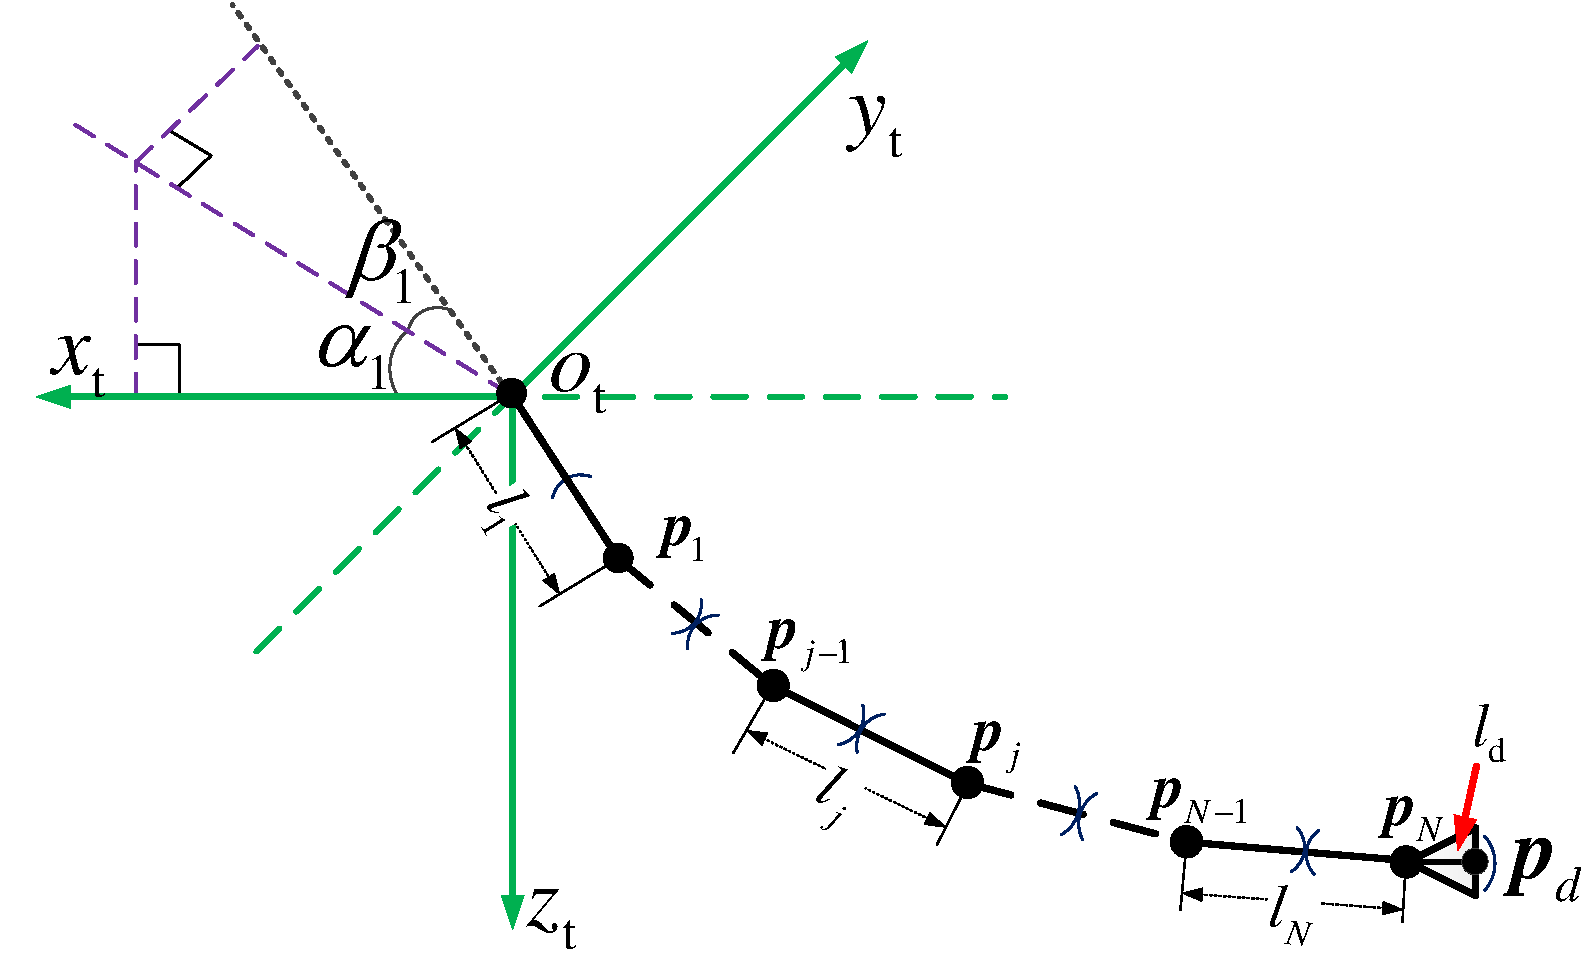
\includegraphics[width=0.5\textwidth]{Figures/Figs_Ch3/fig2.pdf}
	\caption{Link-connected hose-dogue model}\label{fig4.2}
\end{figure}

\subsection{Kinematic Equations}
The link-connected model is established in the tanker coordinate system. Since the rotation of the link around itself is not considered, the direction of each link can be described using two angles, ${\alpha _j},{\beta _j}$, as shown in Fig. \ref{fig4.2}. For example, ${\alpha _1},{\beta _1}$ represent the direction angles of the first link. Then, the relationship between the two spherical joints can be expressed using these direction angles
\begin{equation}\label{eq4.74}
{{{\bf{p}}}_{j /{\left( {j - 1} \right)}}}=  - {l_j}{{{\bf{n}}}_j},j = 1,2, \ldots ,N
\end{equation}
where ${{{\bf{n}}}_j} \in \mathbb{R}^{3}$ represents the direction of the $j$th link and can be obtained from the following equations
\begin{equation}\label{eq4.75}
{{{\bf{n}}}_j}{\rm{ = }}\left[ {\begin{array}{*{20}{c}}
	{\cos {\alpha _j}\cos {\beta _j}}\\
	{\sin {\beta _j}}\\
	{ - \sin {\alpha _j}\cos {\beta _j}}
	\end{array}} \right] \, .
\end{equation}
According to Eq. (\ref{eq4.74}), the position relationship between each mass point can be obtained as follows
\begin{equation}\label{eq4.76}
{{{\bf{p}}}_j} = {{{\bf{p}}}_{j - 1}} + {{\bf{p}}}_{j/(j-1)} ,j = 1,2, \ldots ,N
\end{equation}
Taking the derivative of it, the kinematic relationships between each mass point can be obtained as follows
\begin{equation}\label{eq4.77}
{{{\bf{v}}}_j} = {{{\bf{v}}}_{j - 1}} + {\dot {\bf{p}}}_{j /\left( j - 1\right)} ,{{{\bf{a}}}_j} = {{{\bf{a}}}_{j - 1}} + {\ddot {\bf{p}}}_{j /\left( {j - 1} \right)} ,j = 1,2, \ldots ,N
\end{equation}
where ${\bf{v}}_{j}$ and ${\bf{a}}_{j}$  represent the velocity and acceleration of the $j$th mass point, respectively. Note that since this model is established in the tanker coordinate system, and during the docking process, the tanker coordinate system is equivalent to an inertial frame, the effects of the tanker's motion on the model is not considered in this section. If readers need to consider the influence of the tanker's motion on this model, they can refer to Ref. \cite{ro_modeling_2010}.

As described above, the fundamental variables to represent the link-connected model are the attitude angles of each link. Therefore, the kinematic model should ultimately be expressed in terms of these attitude angles. Thus, expanding Eq. (\ref{eq4.77}), one can obtain
\begin{equation}\label{eq4.78}
{{\dot {\bf{p}}}_{j /\left( {j - 1} \right)}}  =  - {\dot l_j}{{{\bf{n}}}_j} - {l_j}{{\dot {\bf{n}}}_j} =  - {\dot l_j}{{{\bf{n}}}_j} - {l_j}\left( {\frac{{\partial {{{\bf{n}}}_j}}}{{\partial {\alpha _j}}}{{\dot \alpha }_j} + \frac{{\partial {{{\bf{n}}}_j}}}{{\partial {\beta _j}}}{{\dot \beta }_i}} \right)
\end{equation}
\begin{equation}\label{eq4.79}
{{\ddot {\bf{p}}}_{{j/\left( {j - 1} \right)}}} =  - {\ddot l_j}{{{\bf{n}}}_j} - 2{\dot l_j}{{\dot {\bf{n}}}_j} - {l_j}\left( {\frac{{\partial {{{\dot {\bf{n}}}}_j}}}{{\partial {\alpha _j}}}{{\dot \alpha }_j} + \frac{{\partial {{{\dot {\bf{n}}}}_j}}}{{\partial {\beta _j}}}{{\dot \beta }_i}{\rm{ + }}\frac{{\partial {{{\bf{n}}}_j}}}{{\partial {\alpha _j}}}{{\ddot \alpha }_j} + \frac{{\partial {{{\bf{n}}}_j}}}{{\partial {\beta _j}}}{{\ddot \beta }_i}} \right)
\end{equation}
Since ${\bf{n}}_{j}$ represents a direction vector, then
\begin{equation}\label{eq4.80}
\frac{{\partial {{\bf{n}}}_j^\mathrm{T}}}{{\partial {\alpha _j}}} \cdot \frac{{\partial {{{\bf{n}}}_j}}}{{\partial {\beta _j}}} = \frac{{\partial {{\bf{n}}}_j^\mathrm{T}}}{{\partial {\alpha _j}}} \cdot {{{\bf{n}}}_j} = \frac{{\partial {{\bf{n}}}_j^\mathrm{T}}}{{\partial {\beta _j}}} \cdot {{{\bf{n}}}_j} = {\dot {\bf{n}}}_j^\mathrm{T} \cdot {{{\bf{n}}}_j} = 0,\left\| {{{{\bf{n}}}_j}} \right\| = \left\| {{{{\dot {\bf{n}}}}_j}} \right\| = 1
\end{equation}
From Eqs. (\ref{eq4.75}), (\ref{eq4.78}), (\ref{eq4.79}), and (\ref{eq4.80}), one can obtain
\begin{equation}\label{eq4.81}
\left\{ \begin{array}{c}
{{\ddot \alpha }_j} = \frac{1}{{{l_j}}}\frac{{\partial { {{\bf{n}}}_j}}}{{\partial {\alpha _j}}}\left( { - \left( {{ {{\bm{a}}}_j} - { {{\bm{a}}}_{j - 1}}} \right) - 2{{\dot l}_j}{{ {\dot {\bf{n}}}}_j} - {l_j}\left( {\frac{{\partial {{ {\dot {\bf{n}}}}_j}}}{{\partial {\alpha _j}}}{{\dot \alpha }_j} + \frac{{\partial {{ {\dot {\bf{n}}}}_j}}}{{\partial {\beta _j}}}{{\dot \beta }_j}} \right)} \right)\\
{{\ddot \beta }_j} = \frac{1}{{{l_j}}}\frac{{\partial { {{\bf{n}}}_j}}}{{\partial {\beta _j}}}\left( { - \left( {{ {{\bm{a}}}_j} - { {{\bm{a}}}_{j - 1}}} \right) - 2{{\dot l}_j}{{ {\dot {\bf{n}}}}_j} - {l_j}\left( {\frac{{\partial {{ {\dot {\bf{n}}}}_j}}}{{\partial {\alpha _j}}}{{\dot \alpha }_j} + \frac{{\partial {{ {\dot {\bf{n}}}}_j}}}{{\partial {\beta _j}}}{{\dot \beta }_j}} \right)} \right)
\end{array} \right.
\end{equation}
which represents the kinematic equations of the link-connected model.

\subsection{Dynamic Equations}

Air flows over the $j$th link creat frictional drag ${{{\bf{D}}}_{{\rm{F}},j}} \in \mathbb{R}^3$ along the link direction and pressure difference drag ${{{\bf{D}}}_{{\rm{D}},j}} \in \mathbb{R}^3$ perpendicular to the cylinder's direction. The combination of these forces gives the aerodynamic force ${{{\bf{D}}}_{j}} \in \mathbb{R}^3$ acting on the cylinder. For the link-connected model, the dynamic force acting on each link needs to be distributed equally to its two end mass points, so each mass point is subjected to five forces. Define the airspeed of the tanker and eack link as follows
\begin{equation}\label{eq4.82}
{{\bf{v}}}_{{\rm{t/w}}}^{\rm{g}} =  {{\bf{v}}}_{\rm{t}}^{\rm{g}} -  {{\bf{v}}}_{\rm{w}}^{\rm{g}}, {{\bf{v}}}_{j{\rm{/w}}}^{\rm{g}} =  {{\bf{v}}}_{j}^{\rm{g}} -  {{\bf{v}}}_{\rm{w}}^{\rm{g}}
\end{equation}
Among them, ${{\bf{v}}}_{\rm{w}}^{\rm{g}}$ is the local wind speed. As shown in Fig. \ref{fig4.3}, these five forces are the gravity ${{{\bf{G}}}_{j}} \in \mathbb{R}^3$ acting on the mass point, the tension forces ${\mathbf{t}_{j}} \in \mathbb{R}^3,{\mathbf{t}_{j+1}} \in \mathbb{R}^3$ in the two link connectors, and the equivalent forces ${\bf{D}}_{j}/2,{\bf{D}}_{j+1}/2$ due to the aerodynamic forces acting on the two links at that point. For the last mass point $m_{N}$, since the next link is replaced by a drogue, its force situation is different, as shown in Fig. \ref{fig4.4}. The five forces acting on $m_{N}$ are the tension force $t_{N}$ in the $N$th link and its equivalent aerodynamic force ${\bf{D}}_{N}/2$, the gravity of the mass point and the drogue ${{{\bf{G}}}_{N}} \in \mathbb{R}^3,{{{\bf{G}}}_\text{d}} \in \mathbb{R}^3$, and the aerodynamic force ${{{\bf{G}}}_\text{d}} \in \mathbb{R}^3$ acting on the drogue.
\begin{figure}[th]
	\centering
	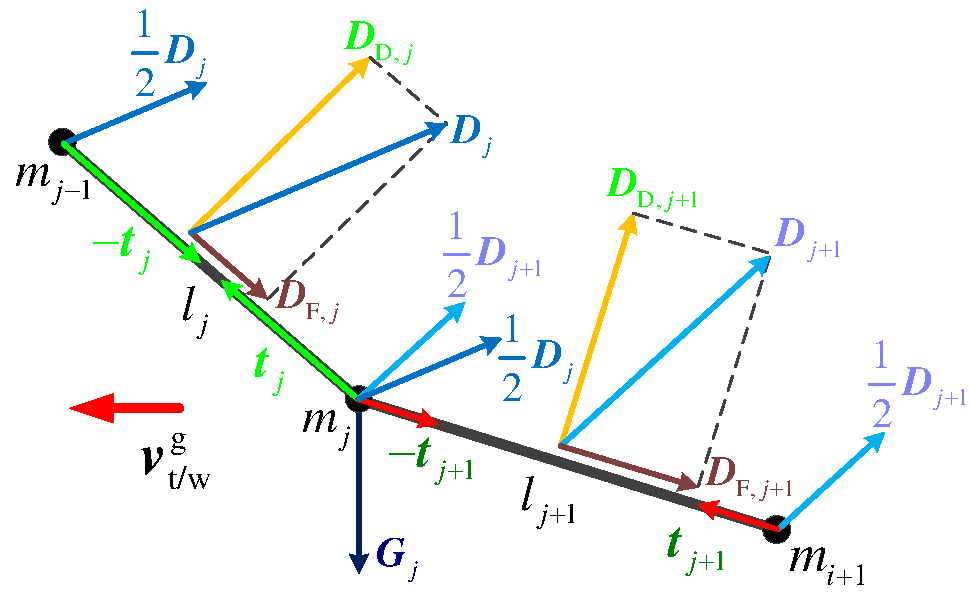
\includegraphics[width=0.5\textwidth]{Figures/Figs_Ch3/fig3.pdf}
	\caption{Analysis of forces on the first $N-1$ links}\label{fig4.3}
\end{figure}
\begin{figure}[th]
	\centering
	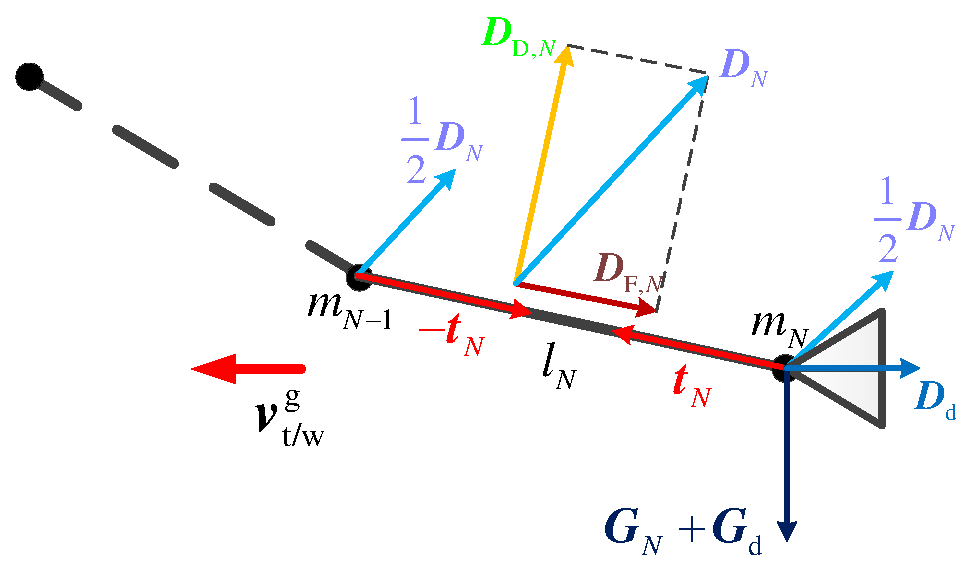
\includegraphics[width=0.5\textwidth]{Figures/Figs_Ch3/fig4.pdf}
	\caption{Analysis of forces on the $N$th link}\label{fig4.4}
\end{figure}

According to aerodynamics principles, the calculation of friction drag and pressure drag is as follows
\begin{equation}\label{eq4.83}
{ {{\bf{D}}}_{{\rm{F}},j}} =  - \left[ {{{\rm{C}}_{{\rm{F}},j}}{\rho _\infty }{{\left( { {{\bf{v}}}_{j{\rm{/w}}}^{\rm{g}} \cdot { \mathbf{n}_{{\rm{F}},j}}} \right)}^2}\left( {\pi {r_j}{l_j}} \right)} \right]{ \mathbf{n}_{{\rm{F}},j}}
\end{equation}
\begin{equation}\label{eq4.84}
{ {{\bf{D}}}_{{\rm{D}},j}} =  - \left[ {{{\rm{C}}_{{\rm{D}},j}}{\rho _\infty }{{\left( {{\mathbf{n}_{{\rm{D}},j}} \cdot {\mathbf {n}_{{\rm{D}},j}}} \right)}^2}\left( {\pi {r_j}{l_j}} \right)} \right]{\mathbf {n}_{{\rm{D}},j}}
\end{equation}
where ${\rho _\infty }$ represents the density of the stationary air at that altitude, and ${\mathbf {n}_{{\rm{F}},j}},{\mathbf {n}_{{\rm{D}},j}}$ are the directions of the two forces, which can be expressed as
\begin{equation}\label{eq4.85}
{\mathbf {n}_{{\rm{F}},j}} = {\mathbf {n}_j},{\mathbf {n}_{{\rm{D}},j}} =  {{\mathbf{v}}}_{j{\rm{/w}}}^{\rm{g}} - \left( { {{\mathbf{v}}}_{j{\rm{/w}}}^{\rm{g}} \cdot {\mathbf {n}_j}} \right){\mathbf {n}_j}
\end{equation}
The parameters ${{\rm{C}}_{{\rm{F}},j}}$ and ${{\rm{C}}_{{\rm{D}},j}}$ represent aerodynamic coefficients. According to Ref. \cite{vassberg_numerical_2003}, before calculating ${{\rm{C}}_{{\rm{F}},j}}$ and ${{\rm{C}}_{{\rm{D}},j}}$, it is necessary to compute the Reynolds number of the fluid at each link's location.
\begin{equation}\label{eq4.86}
{{\mathop{\rm Re}\nolimits} _j} = \frac{{{\rho _j}\left\| { {{\mathbf{v}}}_{j{\rm{/w}}}^{\rm{g}}} \right\|{l_{{\rm{ch}},j}}}}{\upsilon } \approx \frac{{{\rho _\infty }\left\| { {{\mathbf{v}}}_{j/{\rm{w}}}^{\rm{g}}} \right\|{l_{{\rm{ch}},j}}}}{\upsilon }
\end{equation}
where ${\rho _\infty }$ is the local fluid density, and since the airflow compression during the docking process can be neglected, it is approximately equivalent to the density of static atmosphere at that altitude. $\upsilon $ is the dynamic viscosity coefficient of the local atmosphere, and ${l_{{\rm{ch}},j}}$ is the characteristic length of the $j$th link, represented as
\begin{equation}\label{eq4.87}
{l_{{\rm{ch}},j}} = \frac{{\pi {r_{\rm{h}}}}}{{\sin {\vartheta _j}}}
\end{equation}
where ${\vartheta _j}$ is the angle between the link and the airspeed $ {{\mathbf{v}}}_{j{\rm{/w}}}^{\rm{g}}$, and ${r_{\rm{h}}}$ is the outer radius of the hose, i.e.
\begin{equation}\label{eq4.88}
{\vartheta _j} = \arccos \frac{{{\mathbf {n}_j^\mathrm{T}}   {{\mathbf{v}}}_{j{\rm{/w}}}^{\rm{g}}}}{{\left\| {{\mathbf {n}_j}} \right\|\left\| { {{\mathbf{v}}}_{j{\rm{/w}}}^{\rm{g}}} \right\|}} \, .
\end{equation}
After obtaining the Reynolds number, ${{\rm{C}}_{{\rm{F}},j}}$ and ${{\rm{C}}_{{\rm{D}},j}}$ can be determined based on the Reynolds number, as shown in Table \ref{tab4.1}.
\begin{table}[th]
	\caption{The relations among ${{\rm{C}}_{{\rm{F}},j}},{{\rm{C}}_{{\rm{D}},j}}$ and ${{\mathop{\rm Re}\nolimits} _j}$}
	\renewcommand\arraystretch{1.3}
	\centering
	\begin{tabular}	
		[c]{|c|c|c|c|}
		
		\hline
		${{\mathop{\rm Re}\nolimits} _j}$ &${{\rm{C}}_{{\rm{F}},j}}$&${{\mathop{\rm Re}\nolimits} _j}$&${{\rm{C}}_{{\rm{D}},j}}$
		\\\hline
		$\left( {{{10}^{ - 2}},{{10}^4}} \right]$&$4.6409{{\mathop{\rm Re}\nolimits} ^{ - 0.6667}}$&$\left( {{{10}^{ - 2}},1} \right]$&$10{{\mathop{\rm Re}\nolimits} ^{ - 0.81}}$
		\\\hline
		$\left( {{{10}^4},{{10}^{10}}} \right]$ &$0.0464{{\mathop{\rm Re}\nolimits} ^{ - 0.1667}}$&$\left( {1,180} \right]$&$10{{\mathop{\rm Re}\nolimits} ^{ - 0.4083}}$
		\\\hline
		$\left( {{{10}^{10}}, + \infty } \right]$&$0.001$&$\left( {180,4 \times {{10}^5}} \right]$&$1.2$
		\\\hline
		& &$\left( {4 \times {{10}^5},4 \times {{10}^6}} \right]$&$0.002128{{\mathop{\rm Re}\nolimits} ^{ - 0.3522}}$
		\\\hline
		& &$\left( {4 \times {{10}^6}, + \infty } \right]$&$0.45$
		\\\hline
	\end{tabular}
	\label{tab4.1}
\end{table}
Additionally, the drogue also experiences aerodynamic forces. Ref. \cite{ro_aerodynamic_2007} analyzed the aerodynamic forces acting on the drogue and provided the equation for the aerodynamic force on the drogue as follows
\begin{equation}\label{eq4.89}
{ {{\bf{D}}}_{\rm{d}}} = \frac{1}{2}{{\rm{C}}_{\rm{d}}}{\rho _\infty }\left( { {({\mathbf{v}}}_{N{\rm{/w}}}^{\rm{g}})^\mathrm{T}  {{\mathbf{v}}}_{N{\rm{/w}}}^{\rm{g}}} \right)\left( {\pi {r_{\rm{d}}}} \right)\left( {\frac{{ {{\mathbf{v}}}_{N{\rm{/w}}}^{\rm{g}}}}{{\left\| { {{\mathbf{v}}}_{N{\rm{/w}}}^{\rm{g}}} \right\|}}} \right)
\end{equation}
where ${r_{\rm{d}}}$ is the radius of the drogue canopy, and ${{\rm{C}}_{\rm{d}}}$ is a coefficient determined by the drogue strut angle as shown in Fig. \ref{fig4.5} and the canopy area, and so on. Typically, this coefficient is taken as 0.8 \cite{ro_aerodynamic_2007}. At this point, all forces except for the tension are known. The following section provides the method for calculating the tension.
\begin{figure}[th]
	\centering
	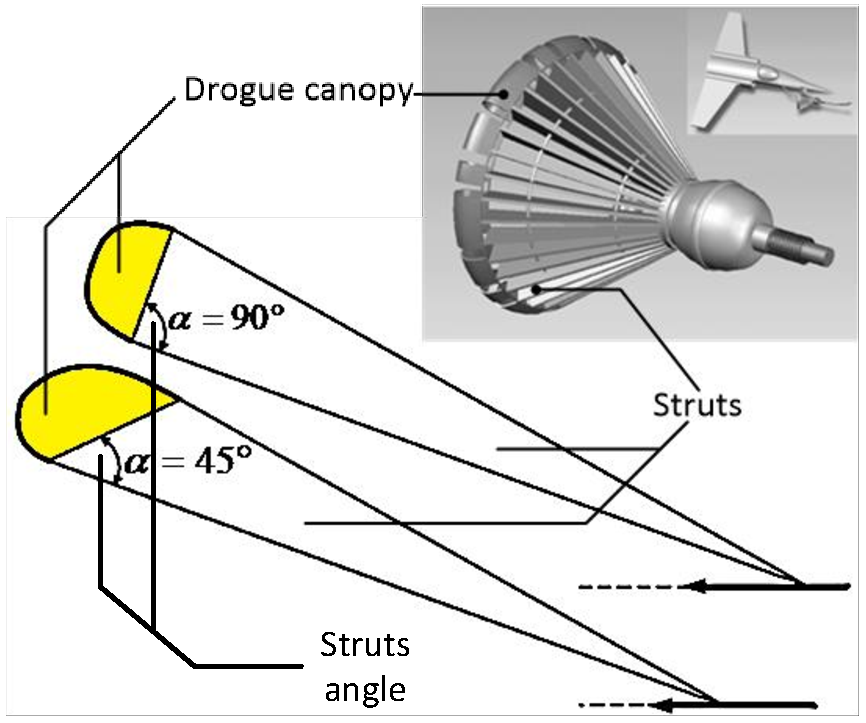
\includegraphics[width=0.5\textwidth]{Figures/Figs_Ch3/fig5.pdf}
	\caption{Drogue canopy's angle of struts}\label{fig4.5}
\end{figure}

\subsection{Calculation of Tension}
In the link-connected model, since the tension force is generated internally within the system, it is considered an internal force, while the other forces are external forces. For ease of calculation, the external forces composed of aerodynamic forces and gravity are denoted as ${{{\bf{Q}}}_j} \in\mathbb{R}^{3} $, i.e,
\begin{equation}\label{eq4.90}
\left\{ \begin{array}{l}
{ {{\bf{Q}}}_j} = {m_j}\bm{g} + \frac{1}{2}\left( {{ {{\bf{D}}}_j} + { {{\bf{D}}}_{j + 1}}} \right),j = 1,2, \ldots ,N - 1\\
{ {{\bf{Q}}}_N} = \left( {{m_N} + {m_{\rm{d}}}} \right) {\bm{g} + }\frac{1}{2}{ {{\bf{D}}}_N} + { {{\bf{D}}}_{\rm{d}}} + {\mathbf{F}_{\rm{b}}}\, .
\end{array} \right.
\end{equation}
Assume the tension at the two ends of the same link is ${t_j}{ {{\mathbf{n}}}_j}$ and $ - {t_j}{ {{\mathbf{n}}}_j}$, where ${t_j}$ is a constant, which satisfies the property that the tension at both ends of the link has the same magnitude, opposite direction, and along the link. Here, ${\mathbf{F}_{\rm{b}}}$ represents other external disturbances acting on the drogue, and it actually includes the bow wave, which is included in the external forces acting on the last mass point. Therefore, according to Newton's second law, one has
\begin{equation}\label{eq4.91}
\left\{ \begin{array}{l}
{ {{\bf{a}}}_j} = \frac{{{t_j}{ {{\mathbf{n}}}_j} - {t_{j + 1}}{ {{\mathbf{n}}}_{j + 1}} + { {{\bf{Q}}}_j}}}{{{m_j}}},j = 1,2, \ldots ,N - 1\\
{ {{\bf{a}}}_N} = \frac{{{t_N}{ {{\mathbf{n}}}_N} + { {{\bm{Q}}}_N}}}{{{m_N}}}
\end{array} \right.
\end{equation}
where ${ {{\bf{a}}}_j}$ represents the acceleration of the $j$th link, and ${ {{\bf{a}}}_N}$ represents the acceleration of the drogue.

On the other hand, since
\begin{equation}\label{eq4.92}
\mathbf{p}_{{j/ {\left( {j - 1} \right)}}}^\mathrm{T} \cdot {\mathbf {p}_{{j /{\left( {j - 1} \right)}}}} = l_j^2
\end{equation}
Taking the second derivative of both sides of this equation, it can be obtained
\begin{equation}\label{eq4.93}
{{\mathbf{n}}}_j^\mathrm{T} \cdot \left( {{ {{\bf{a}}}_j} - { {{\bf{a}}}_{j - 1}}} \right) = {l_j} {\dot {\mathbf{n}}}_j^\mathrm{T}{ {\dot {\mathbf{n}}}_j} - {\ddot l_j}
\end{equation}
Therefore, by combining Eq. (\ref{eq4.91}) and Eq. (\ref{eq4.93}) and rearranging them
\begin{equation}\label{eq4.94}
{\bf{T}}^\mathrm{T}   {\bf{t} = \bm{q}}
\end{equation}
where $ {\bf{t} = }{\left[ {\begin{array}{*{20}{c}}
		{{t_1}}&{{t_2}}& \cdots &{{t_N}}
		\end{array}} \right]^{\rm{T}}}$, and the coefficient matrix ${\bf{T}}$ is known in terms of $\bm{q}$ (its specific form will be described in the next section). With this, the relationship between internal force and external force can be established. By solving Eq. (\ref{eq4.91}), we can obtain ${\bm{a}}_{j}$ and then update it in Eq. (\ref{eq4.81}). This completes the entire link-connected model.

The block diagram of the link-connected hose-drogue model can be obtained based on the above steps, as shown in the Fig. \ref{fig4.6}.
\begin{figure}[th]
	\centering
	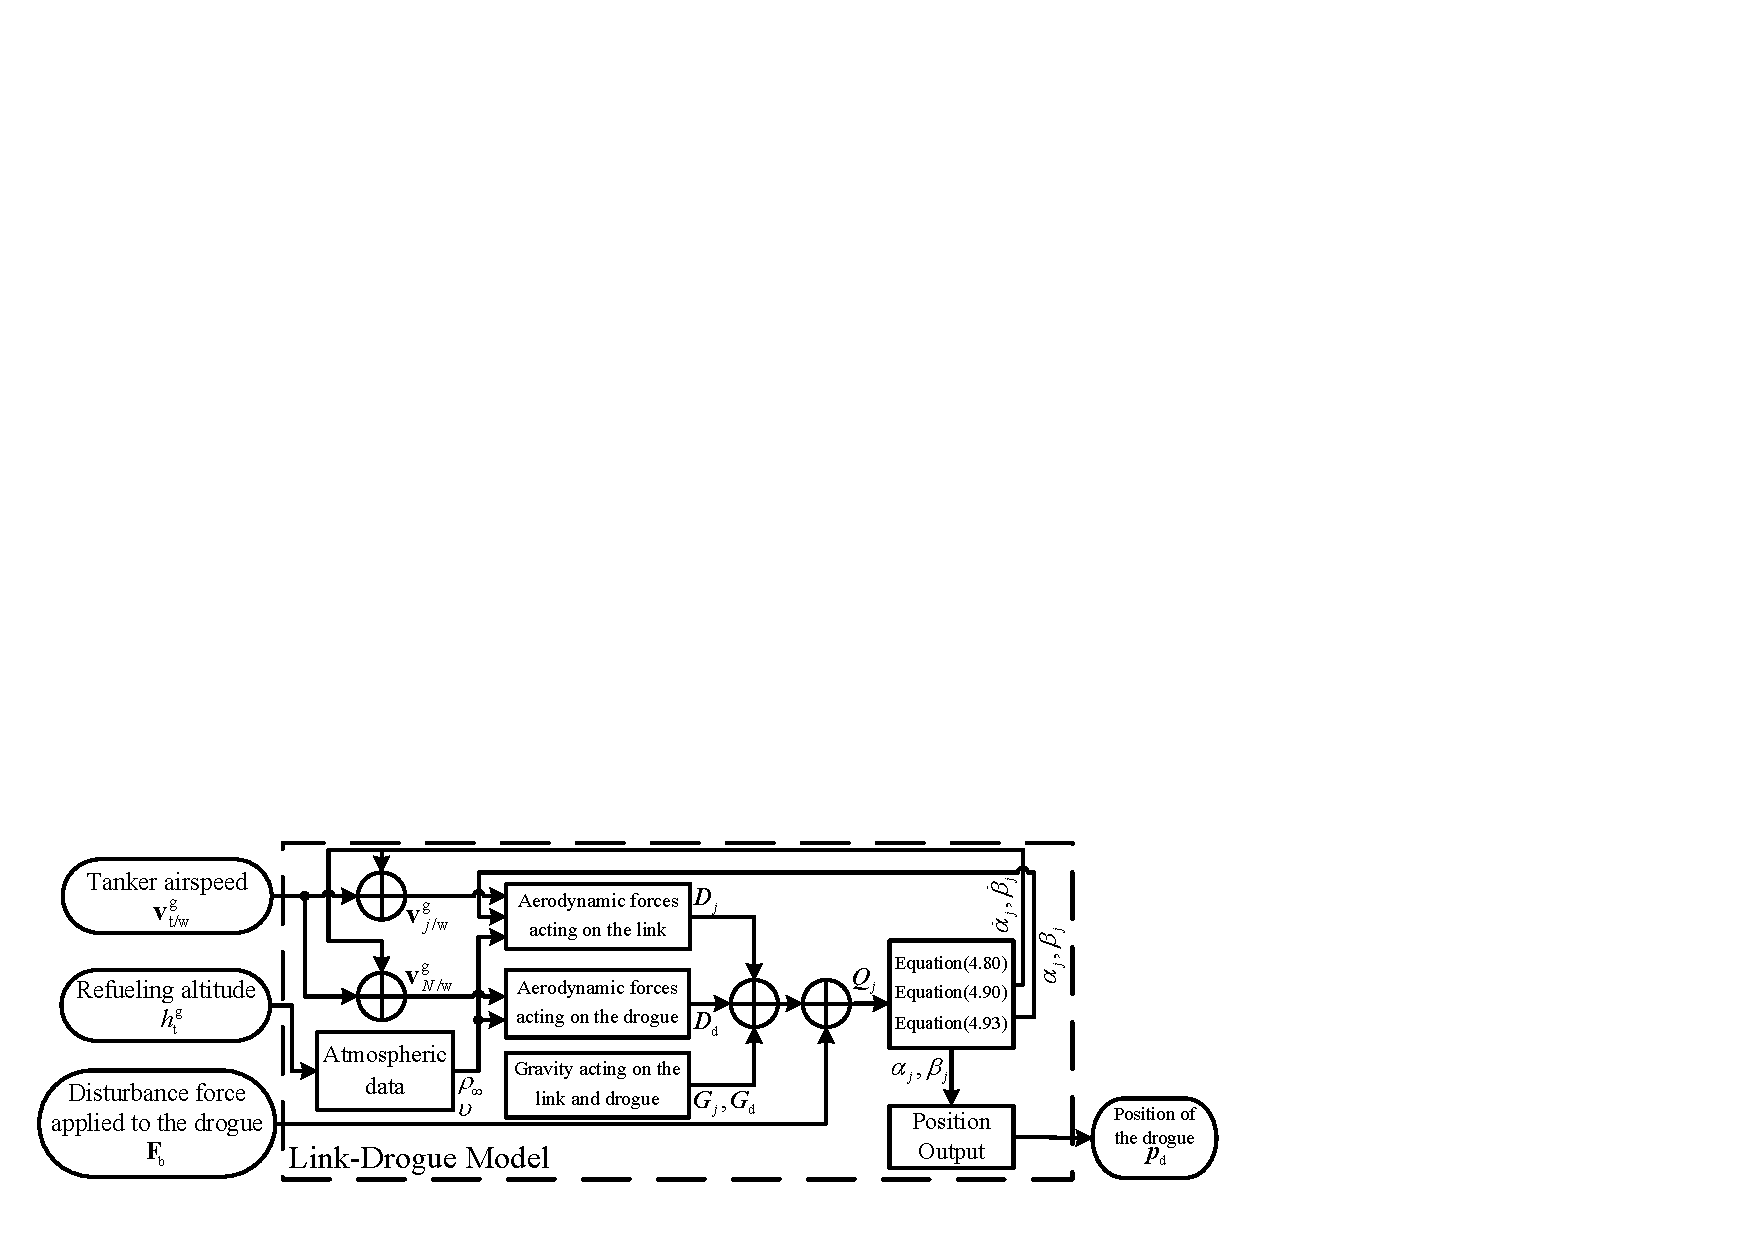
\includegraphics[width=0.9\textwidth]{Figures/Figs_Ch3/fig6.pdf}
	\caption{Flowchart of the link-connected hose-drogue model calculation}\label{fig4.6}
\end{figure}

\subsection{Link-connected Model during Hose Contraction}
It should be noted that due to the presence of the Hose Drum Unit (HDU) in the system, the hose-drogue may retract a certain distance into the refueling pod when subjected to strong disturbances. For the subsequent modeling needs, it is necessary to consider the retraction of the link. If the retraction distance of the link is less than the length of the first link, we will consider the equation for the tension of $N$ links. However, if the disturbances are significant and the retraction length exceeds the length of the first link, the order of the equation will change. Assume that the link visible outside the HDU is the original $i$th link, then Eq. (\ref{eq4.94}) satisfies the following form
\begin{equation}\label{eq4.95}
\left[ {\begin{array}{*{20}{c}}
	{{{\bf{0}}_{\left( {i - 1} \right) \times \left( {i - 1} \right)}}}&{\bf{0}}\\
	{\bf{0}}&{{{{\bf{\bar T}}}_{\left( {N - i + 1} \right) \times \left( {N - i + 1} \right)}}}
	\end{array}} \right] {\bf{t} = }\left[ {\begin{array}{*{20}{c}}
	{{{\bf{0}}_{\left( {i - 1} \right) \times 1}}}\\
	{{{ {\bar {\bm{q}}}}_{\left( {N - i + 1} \right) \times 1}}}
	\end{array}} \right]
\end{equation}
where ${\bf{\bar{ T}}}$ and ${\bar{\bm{q}}}$ are as follows
%where ${\bf{\bar {T}}}$ and $ {\bar {\bm{q}}}$ are as follows:
\begin{equation}\label{eq4.96}
{\bf{\bar T}} = \left[ {\begin{array}{*{20}{c}}
	1&{ - { {{\bf{n}}}^\mathrm{T}_i}{ {{\bf{n}}}_{i{\rm{ + }}1}}}&0& \cdots & \cdots \\
	{ - {\mu _i}{ {{\bf{n}}}^\mathrm{T}_i}{ {{\bf{n}}}_{i + 1}}}&{{\mu _i} + {\mu _{i + 1}}}&{ - {\mu _{i + 1}}{ {{\bf{n}}}^\mathrm{T}_{i + 1}}{ {{\bf{n}}}_{i{\bf{ + }}2}}}&0& \cdots \\
	0& \ddots &0& \cdots & \cdots \\
	0&{ - {\mu _{j - 1}}{ {{\bf{n}}}^\mathrm{T}_{j - 1}}{ {{\bf{n}}}_j}}&{{\mu _{j - 1}} + {\mu _j}}&{{\mu _j}{ {{\bf{n}}}^\mathrm{T}_j}{ {{\bf{n}}}_{j + 1}}}&0\\
	0& \cdots & \ddots &0& \cdots \\
	0&0&{ - {\mu _{N - 2}}{ {{\bf{n}}}^\mathrm{T}_{N - 2}}{ {{\bf{n}}}_{N - 1}}}&{{\mu _{N - 2}} + {\mu _{N - 1}}}&{{\mu _{N - 1}}{ {{\bf{n}}}^\mathrm{T}_{N - 1}}{ {{\bf{n}}}_N}}\\
	0& \cdots & \cdots &{ - {\mu _{N - 1}}{ {{\bf{n}}}^\mathrm{T}_{N - 1}}{ {{\bf{n}}}_N}}&{{\mu _{N - 1}} + {\mu _N}}
	\end{array}} \right]
\end{equation}
\begin{equation}\label{eq4.97}
{\bar {\bm{q}}} = \left[ {\begin{array}{*{20}{c}}
	{{m_i}{l_i}{{\dot {\mathbf{n}}}}_i^2 - {{\mathbf{Q}}^\mathrm{T}_i}{{\mathbf{n}}_i} - {m_i}{{\ddot l}_i}}\\
	{{l_{i + 1}}{\bm{\dot \mathbf {n}}}_{i + 1}^2 + \left( {{\mu _i}{{\mathbf{Q}}^\mathrm{T}_i} - {\mu _{i + 1}}{{\mathbf{Q}}^\mathrm{T}_{i + 1}}} \right){{\mathbf{n}}_{i + 1}}}\\
	\vdots \\
	{{l_j}{\bm{\dot \mathbf {n}}}_j^2 + \left( {{\mu _{j - 1}}{{\mathbf{Q}}^\mathrm{T}_{j - 1}} - {\mu _j}{{\mathbf{Q}}^\mathrm{T}_j}} \right){{\bf{n}}_j}}\\
	\vdots \\
	{{l_{N - 1}}{\bm{\dot\mathbf{n}}}_{N - 1}^2 + \left( {{\mu _{N - 2}}{{\mathbf{Q}}^\mathrm{T}_{N - 2}} - {\mu_{N - 1}}{{\mathbf{Q}}^\mathrm{T}_{N - 1}}} \right){{\mathbf{n}}_{N - 1}}}\\
	{{l_N}{\bm{\dot \mathbf {n}}}_N^2 + \left( {{\mu _{N - 1}}{{\mathbf{Q}}^\mathrm{T}_{N - 1}} - {\mu _N}{{\mathbf{Q}}^\mathrm{T}_N}} \right){{\mathbf{n}}_N}}
	\end{array}} \right]
\end{equation}
where ${\mu _j} = 1 / {{m_j}}$, and when $i = 1$, ${\bf{\bar T}} = {\bf{T}}$ and ${\bar {\bm{q}} = {\bm{q}}}$, and in this case only the first link changes.
The equation for the $i$th link being retracted exactly is 
\begin{equation}\label{eq4.98}
{t_i} - { {{\bf{n}}}^\mathrm{T}_i}{ {{\bf{n}}}_{i + 1}}{t_{i + 1}} = 0 \Rightarrow {t_i} = { {{\bf{n}}}^\mathrm{T}_i}{ {{\bf{n}}}_{i + 1}}{t_{j + 1}}
\end{equation}
This means that at this moment, the length of the link is exactly zero, the mass of the link is zero, and the aerodynamic force acting on it is also zero. On the other hand, due to the continuity of the hose, it can be assumed that its direction is aligned with the next link, and the magnitude of the tension is the same. It is seen that Eq. (\ref{eq4.98}) corresponds well to this physical process. During numerical simulations, the updating process of the calculation for the first link is illustrated by Fig. \ref{fig4.7}.
\begin{figure}[th]
	\centering
	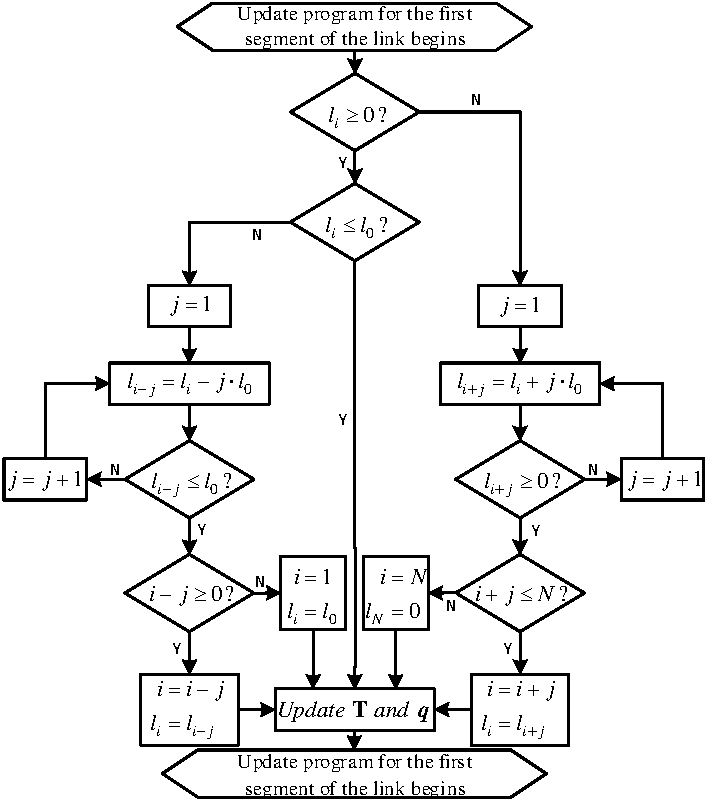
\includegraphics[width=0.7\textwidth]{Figures/Figs_Ch3/fig7.pdf}
	\caption{Updating Process of the First Link}\label{fig4.7}
\end{figure}

In the figure, ${l_0}$ represents the length of each link when it is fully extended, $j$ is the counter, and $j{l_0}$ represents the total length of $j$ links of the hose that are either retracted or extended. This process takes into account situations where the first link cannot be extended any further after being fully extended, and the last link cannot be retracted any further after being fully retracted. It also considers the possibility of encountering numerical calculation scenarios where multiple links of the hose are retracted or extended in a single step.

\subsection{Simulation Example of the link-connected hose-drogue model}

To validate the effectiveness of the link-connected model, simulations are conducted using the parameters listed in Table \ref{tab4.2}. In the table, the variable ${\rho _{\rm{h}}}$ represents the linear density of the hose, and the aerodynamic parameter ${{\rm{C}}_{\rm{d}}}$ for the drogue is typically set to 0.8. It is important to note that in this simulation, the elongation of the hose due to the Hose Drum Unit (HDU) model has not been taken into account.
\begin{table}[th]
	\caption{Simulation Parameters of the link-connected hose-drogue model}
	\renewcommand\arraystretch{1.3}
	\centering
	\begin{tabular}	
		[c]{|c|c|c|c|c|c|}
		
		\hline
		Parameters&Values&Units&Parameters&Values&Units
		\\\hline
		$ {v}_{\rm{t}}^{\rm{g}}$&${\left[ {\begin{array}{*{20}{c}}
				{120}&0&0
				\end{array}} \right]^{\rm{T}}}$&${m/s}$&${l_{\rm{d}}}$&$0.422$&$m$
		\\\hline
		$h_{\rm{t}}^{\rm{g}}$&$3000$& $m$&${l_{\rm{h}}}$&$15$&$m$
		\\\hline
		${\rho _\infty }$&$0.8443$&${{kg} /{{m^3}}}$&${r_{\rm{h}}}$&$0.034$&$m$
		\\\hline
		$\upsilon $&$1.7894 \times {10^{{\rm{ - }}5}}$&${{{m^2}} /s}$&${\rho _{\rm{h}}}$&$4.1$&${{kg} /m}$
		\\\hline
		${r_{\rm{d}}}$&$0.305$&$m$&$N$&$20$&-
		\\\hline
		${m_{\rm{d}}}$&$29.5$&$kg$&$ {w}_{\rm{t}}^{\rm{g}}$&${\left[ {\begin{array}{*{20}{c}}
				0&0&0
				\end{array}} \right]^{\rm{T}}}$&$m/s$
		\\\hline
	\end{tabular}
	\label{tab4.2}
\end{table}

(1) Simulation 1: Windless Scenario

In this simulation, the hose is allowed to fall freely from a horizontal position under no wind conditions. Specifically, when the wind velocity $ {\bf{w}}_{\rm{t}}^{\rm{g}} = {\left[ {\begin{array}{*{20}{c}}
		0&0&0
		\end{array}} \right]^{\rm{T}}}$, the hose is fully extended, and the initial conditions for each link are set to ${\alpha _j}\left( 0 \right) = {\beta _j}\left( 0 \right) = {0^ \circ },j = 1,2, \ldots ,N$. The model is then allowed to move freely, and the trajectories of the links and the drogue are observed. The simulation results are depicted in Fig. \ref{fig4.8}. Since there is no crosswind in this simulation, the position in the ${y_{\rm{t}}}$-direction remains unchanged. Observing the dynamic process, the model reaches a steady state around 20 seconds. Therefore, a moment beyond 20 seconds can be chosen as the equilibrium point of the model under the environmental conditions specified in Table \ref{tab4.2}.

(2) Simulation 2: Drogue Located at Equilibrium Position

In this simulation, the hose is initially at its equilibrium position, and a lateral perturbation is applied to the drogue at 10 seconds. Specifically, the stable state obtained from Simulation 1 is used as the initial condition for Simulation 2. At 10 seconds, a step disturbance is introduced to the system by setting the force ${{\bf{F}}_{\rm{b}}}$ to increase from ${\left[ {\begin{array}{*{20}{c}}
		0&0&0
		\end{array}} \right]^{\rm{T}}}$ to ${\left[ {\begin{array}{*{20}{c}}
		0&{50}&0
		\end{array}} \right]^{\rm{T}}}$ (Unit is N) . The trajectories of the links and the drogue under this scenario are observed. Fig. \ref{fig4.9} illustrates the trajectory of the drogue in this scenario.

From Fig. \ref{fig4.9} (d), it can be observed that under the crosswind perturbation, the drogue first swings in the direction of the wind and upwards. Subsequently, it oscillates back, forming a spiral motion, and finally stabilizes at a new equilibrium position. Moreover, Figs. \ref{fig4.9} (a)-(c) show that the dynamics of the drogue in various directions resemble those of a second-order or even higher-order linear system. This observation serves as the foundation for simplifying the model in subsequent chapters.
\begin{figure}[th]
	\centering
	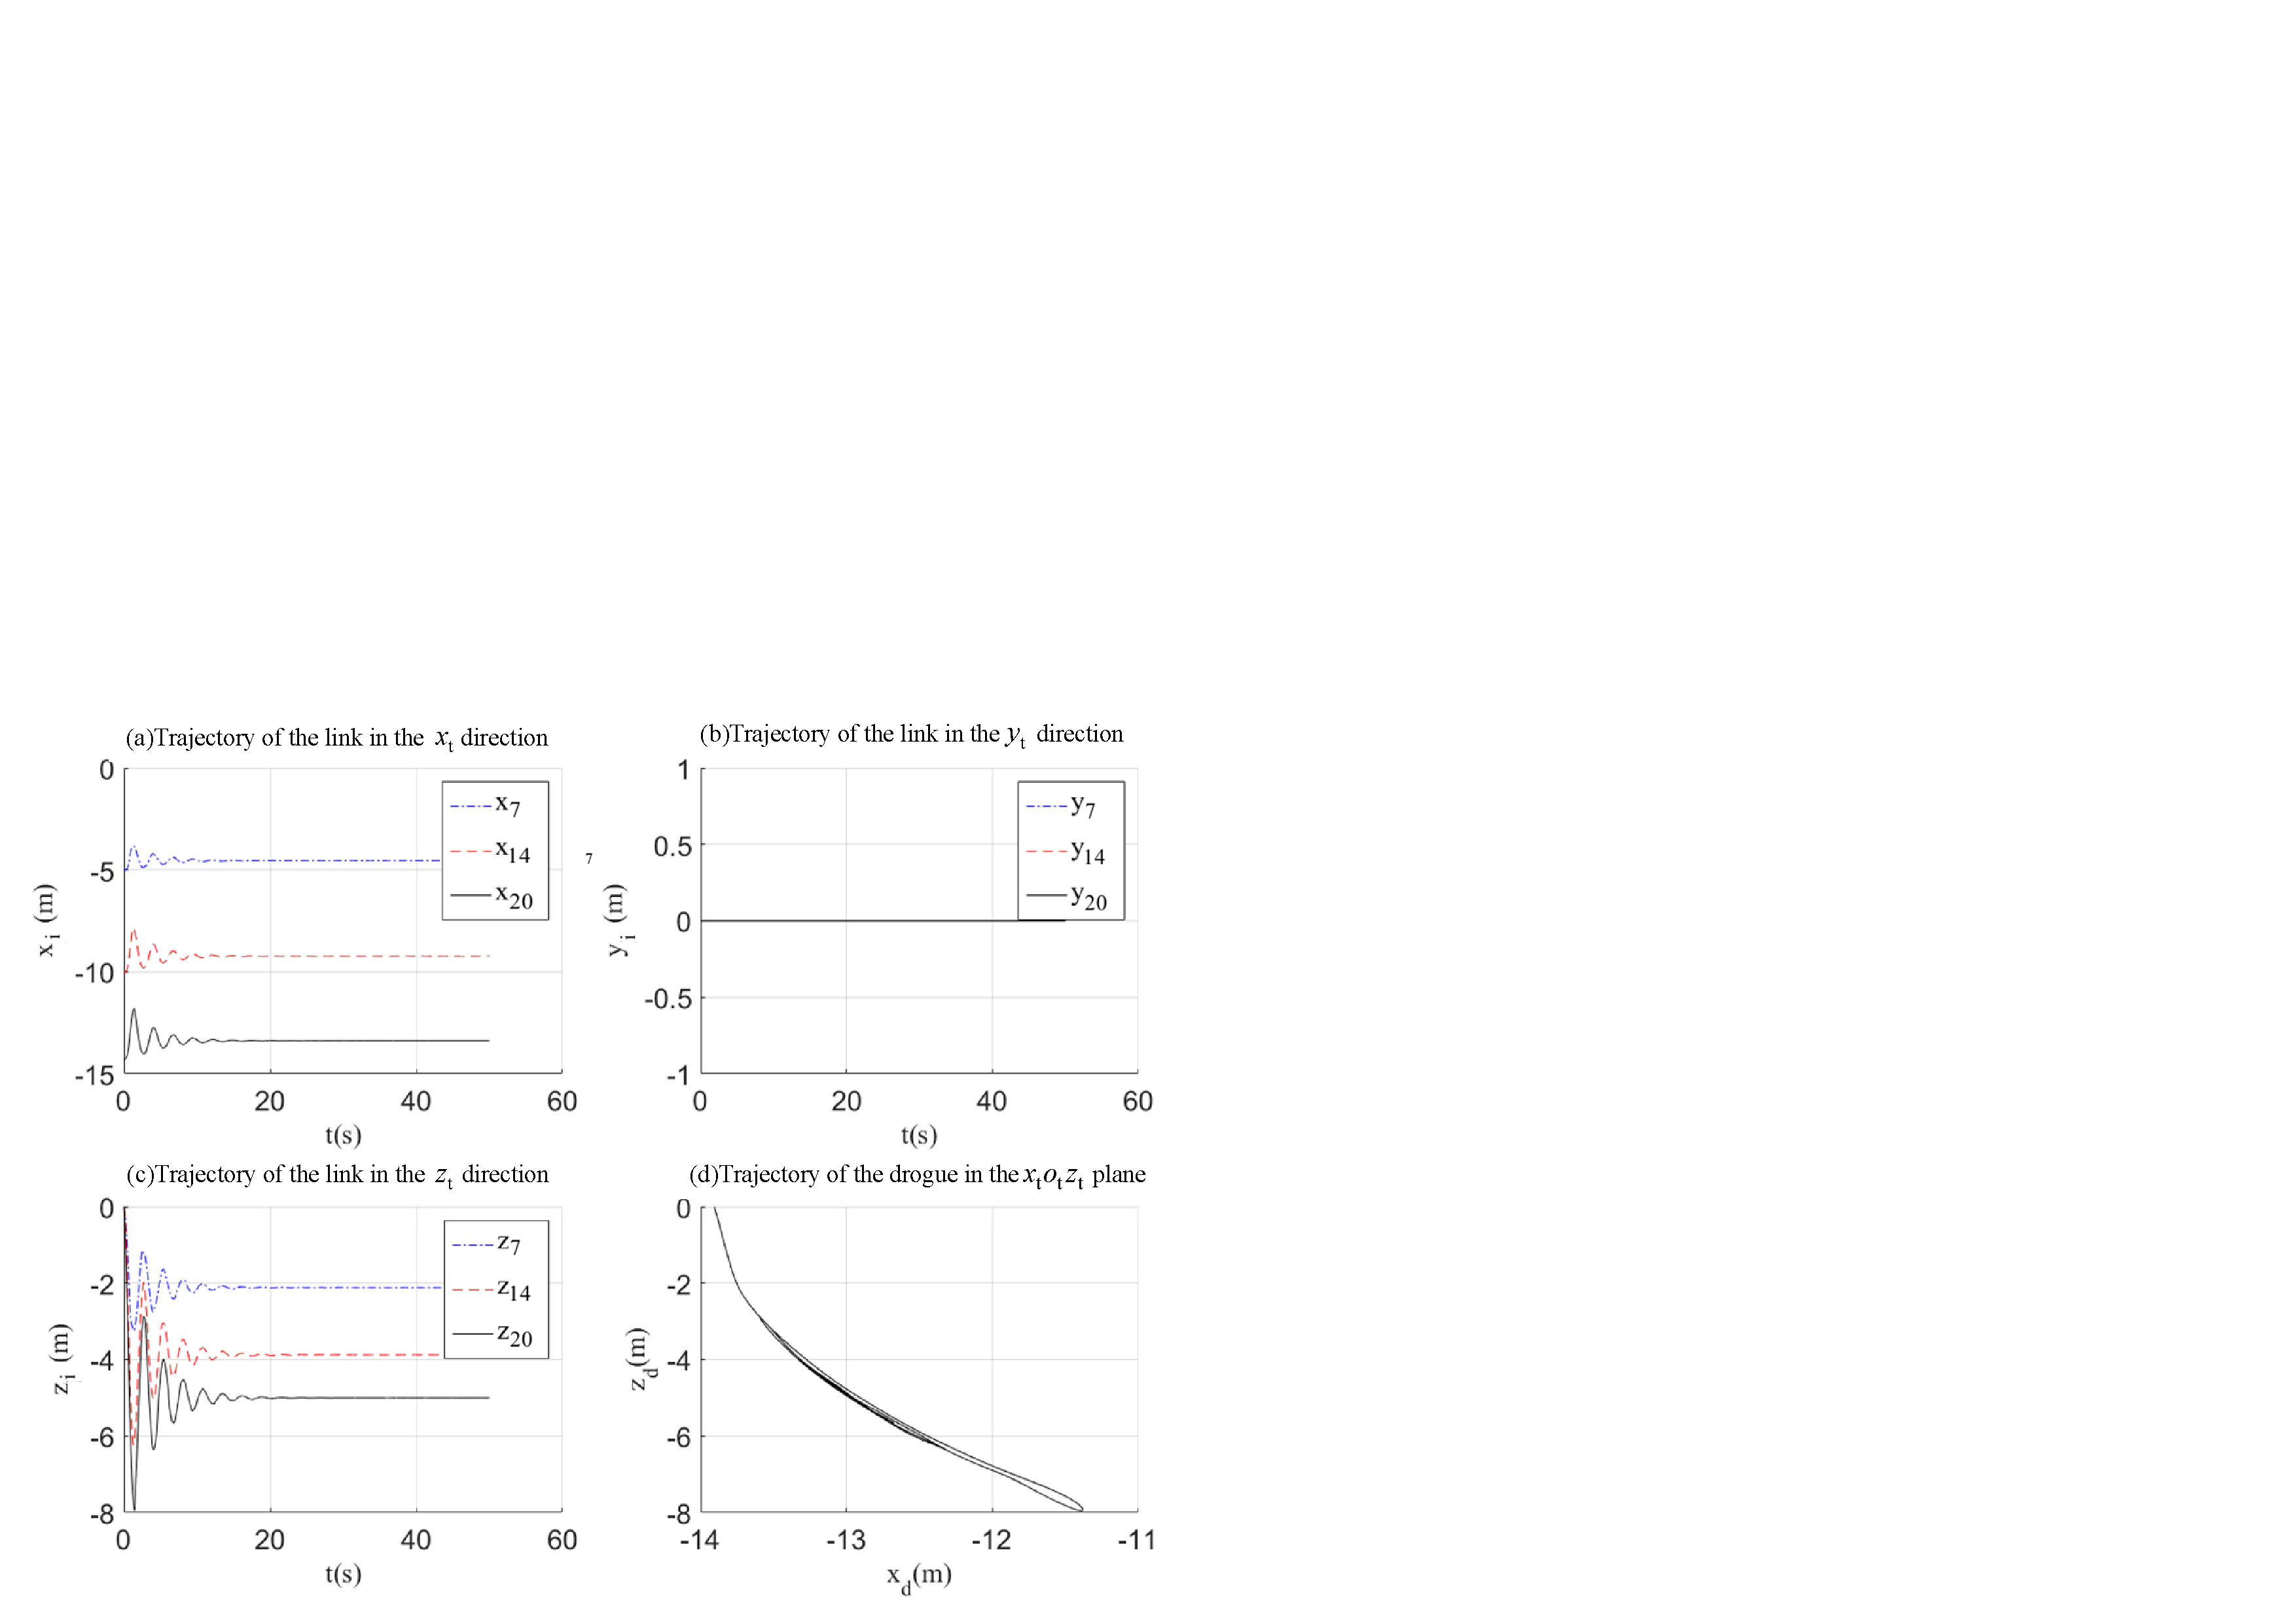
\includegraphics[width=0.8\textwidth]{Figures/Figs_Ch3/fig8.pdf}
	\caption{Simulation 1: Trajectory of the Hose in Free Fall without Wind}\label{fig4.8}
\end{figure}
\begin{figure}[th]
	\centering
	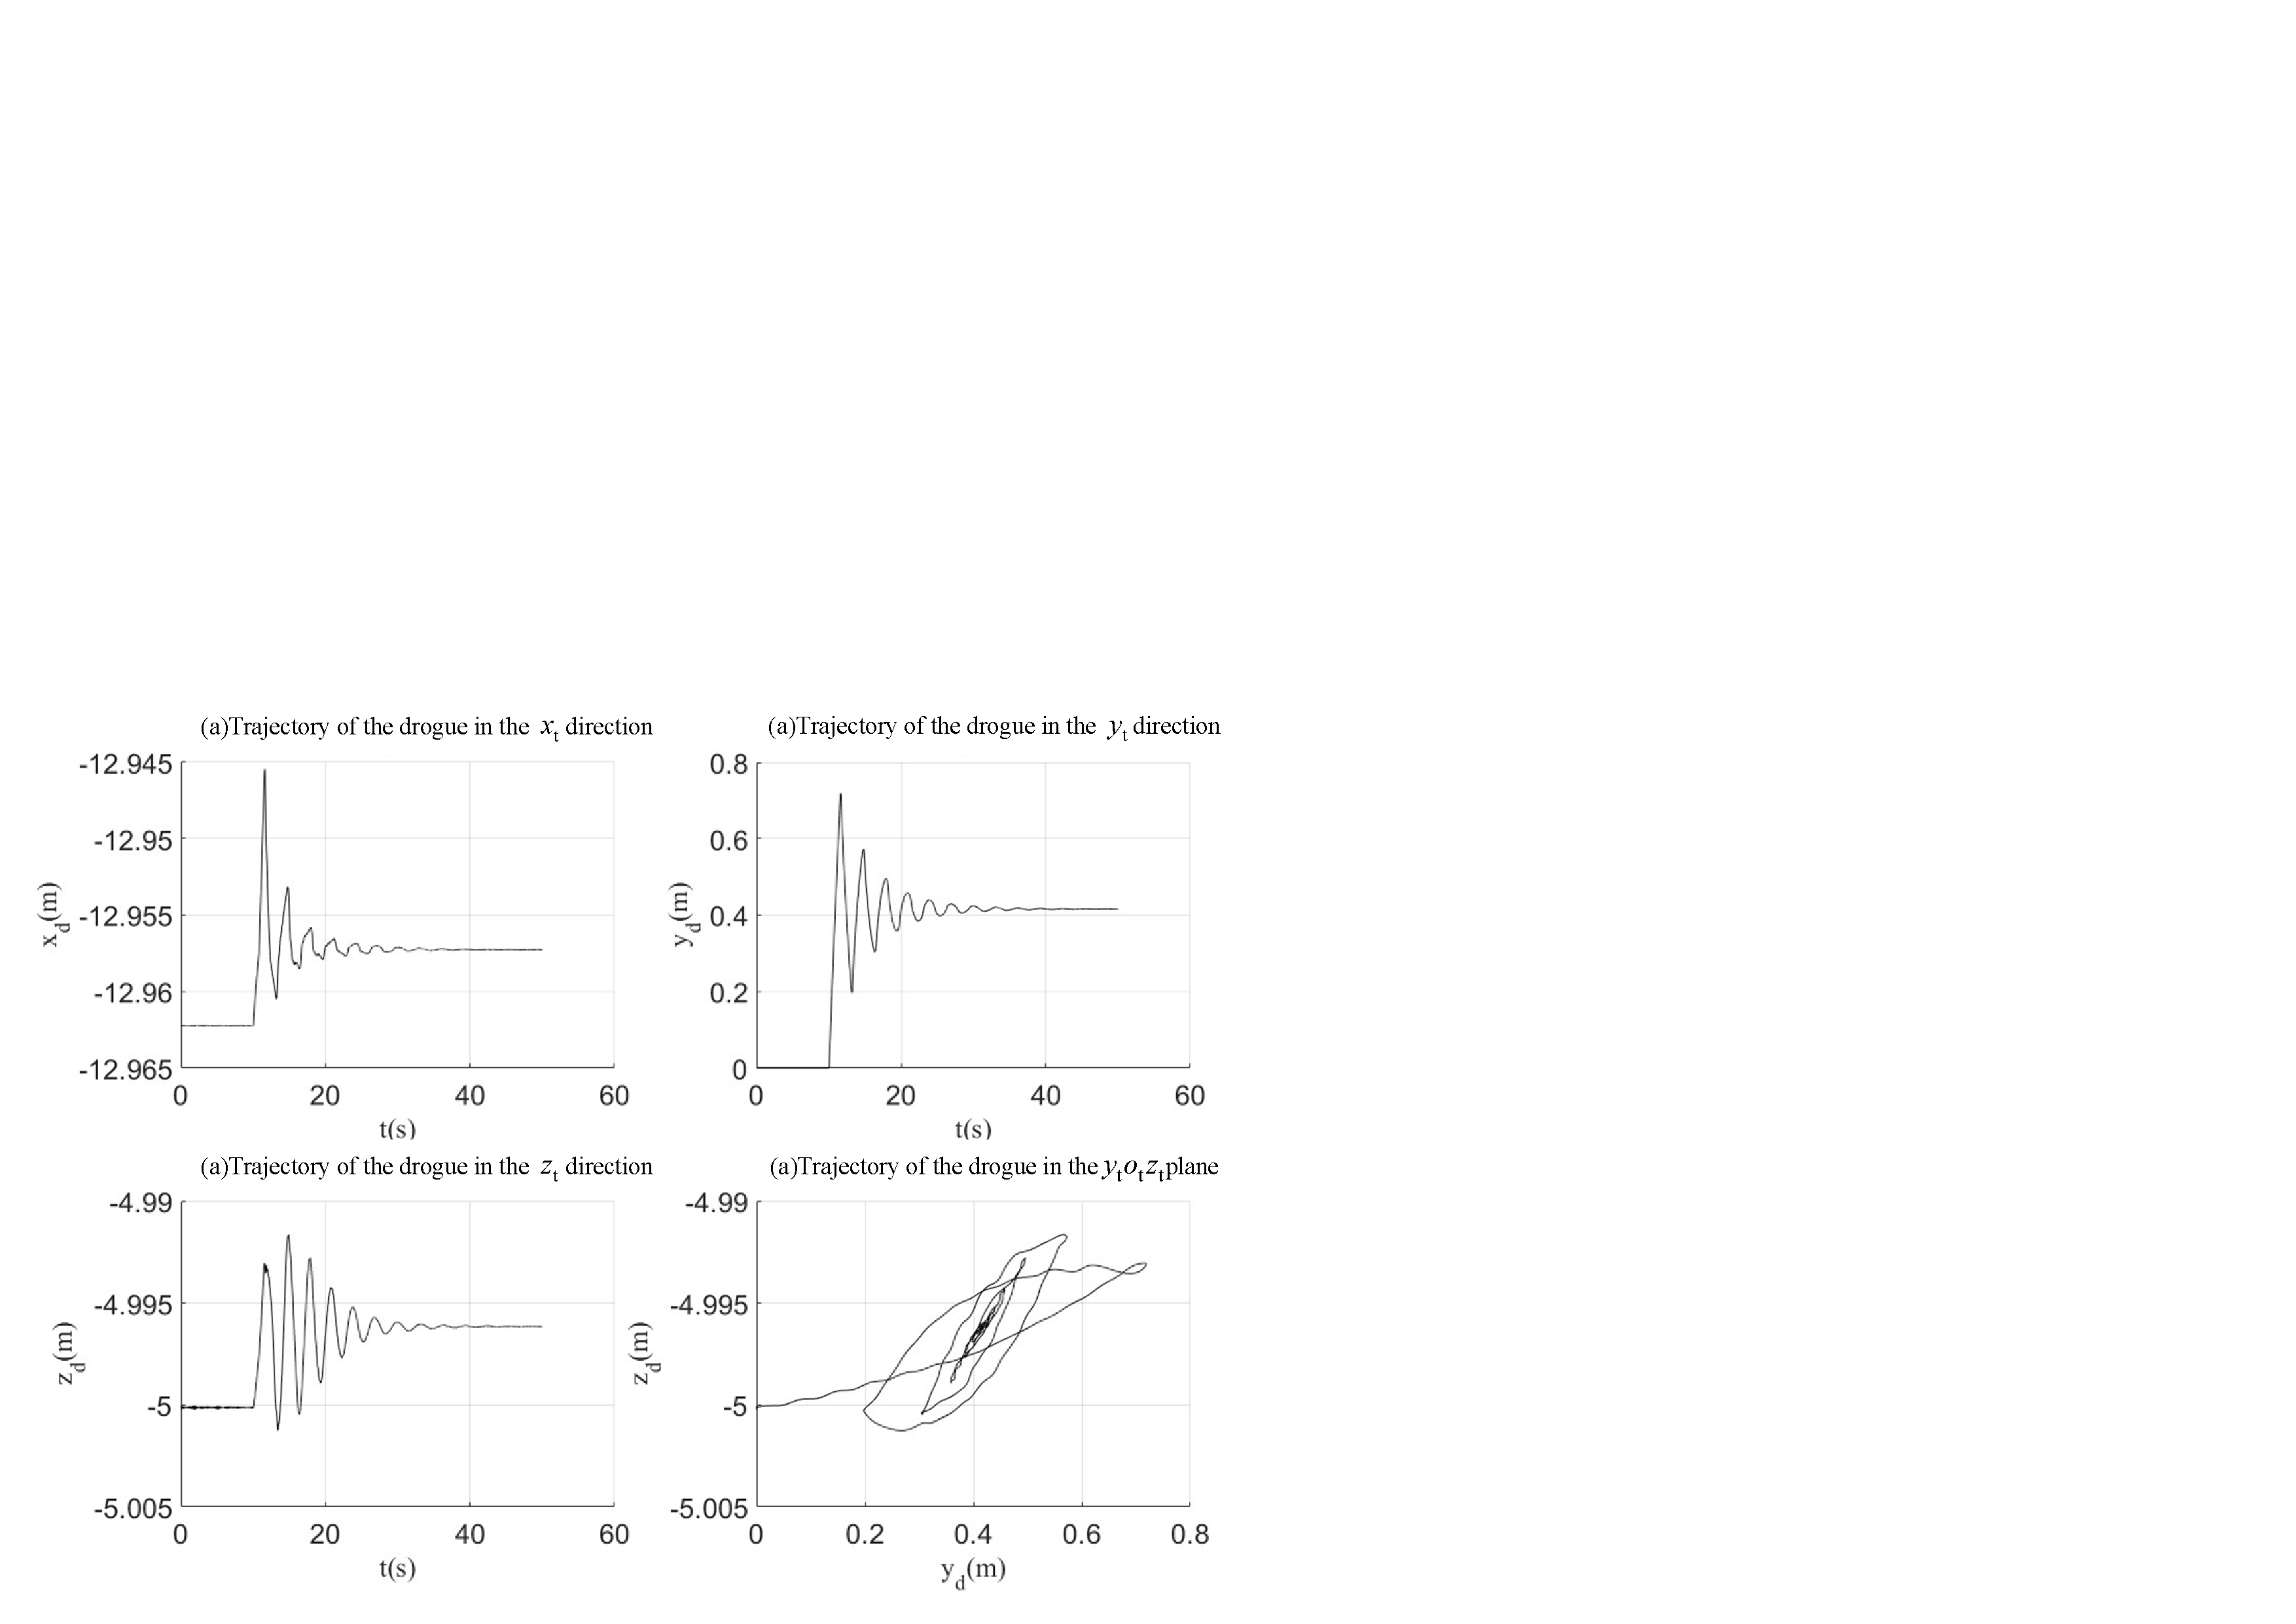
\includegraphics[width=0.8\textwidth]{Figures/Figs_Ch3/fig9.pdf}
	\caption{Simulation 2: Trajectory of the Drogue Under Crosswind Conditions}\label{fig4.9}
\end{figure}

%\section{Drogue Dynamic Model with HDU}
%In the probe-and-drogue refueling system, a device is installed at the front end of the hose to release or withdraw the hose, known as the Hose Drum Unit (HDU), also referred to as the Reel Take-Up System. This unit is situated within the refueling pod, as shown in Fig. \ref{fig4.22}. The HDU primarily consists of a drum (reel) that winds the hose, a motor responsible for controlling the rotation of the drum, and a controller for the motor. The rotation of the motor is primarily controlled based on the status of the upper end of the hose connected to the refueling pod. This device regulates the hose tension by adjusting the length of the hose exposed outside when the hose tension is insufficient. It effectively mitigates the phenomenon of hose whipping by reducing the risk of sudden tension changes, thereby minimizing potential refueling accidents caused by such effects.
%\begin{figure}[th]
%	\centering
%	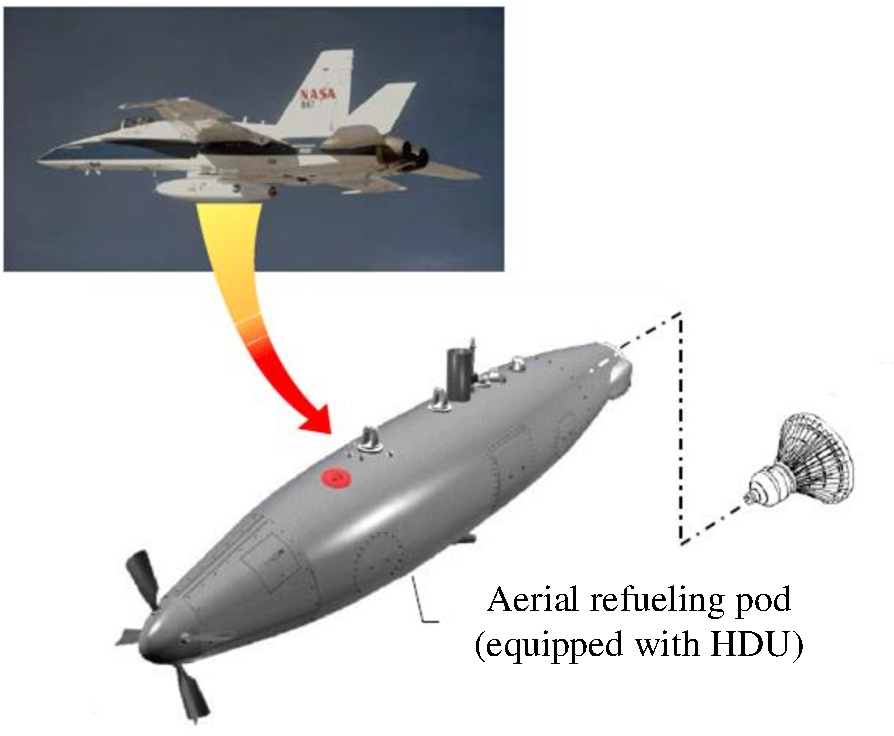
\includegraphics[width=0.6\textwidth]{Chap4/fig22.pdf}
%	\caption{Refueling Pod and HDU Schematic}\label{fig4.22}
%\end{figure}
%Currently, research on the HDU primarily focuses on designing controllers to regulate the hose tension and suppress hose whipping phenomenon. Hose whipping usually occurs after the docking of the drogue and probe, but the HDU's role in suppressing hose whipping also affects the dynamics of the hose-drogue assembly during the docking process. However, this aspect has received relatively little attention in current research. Therefore, this section will provide an initial analysis of this impact.
%
%\subsection{Analysis of Fixed-Length link-connected model Deficiencies}
%
%Based on the analysis in Section 4.3.4, the significant downward movement of the drogue in the ${o_{\rm{t}}}{z_{\rm{t}}}$ direction compared to the experiment can be observed. From this phenomenon and the corresponding time of occurrence, it can be inferred that this dynamic motion of the drogue in the ${o_{\rm{t}}}{z_{\rm{t}}}$ direction is caused by the component of the bow wave in the ${o_{\rm{t}}}{x_{\rm{t}}}$ direction, meaning that the force in the ${o_{\rm{t}}}{x_{\rm{t}}}$ direction induces a substantial displacement of the drogue in the ${o_{\rm{t}}}{z_{\rm{t}}}$ direction. The reason behind this phenomenon is that the hose-drogue system is under tension when in a steady state, making the hose behave more rigidly. The hose-drogue system is approximately similar to a simple pendulum near its equilibrium position \cite{williamson_controllable_2010}, as depicted in Fig. \ref{fig4.23}.
%\begin{figure}[th]
%	\centering
%	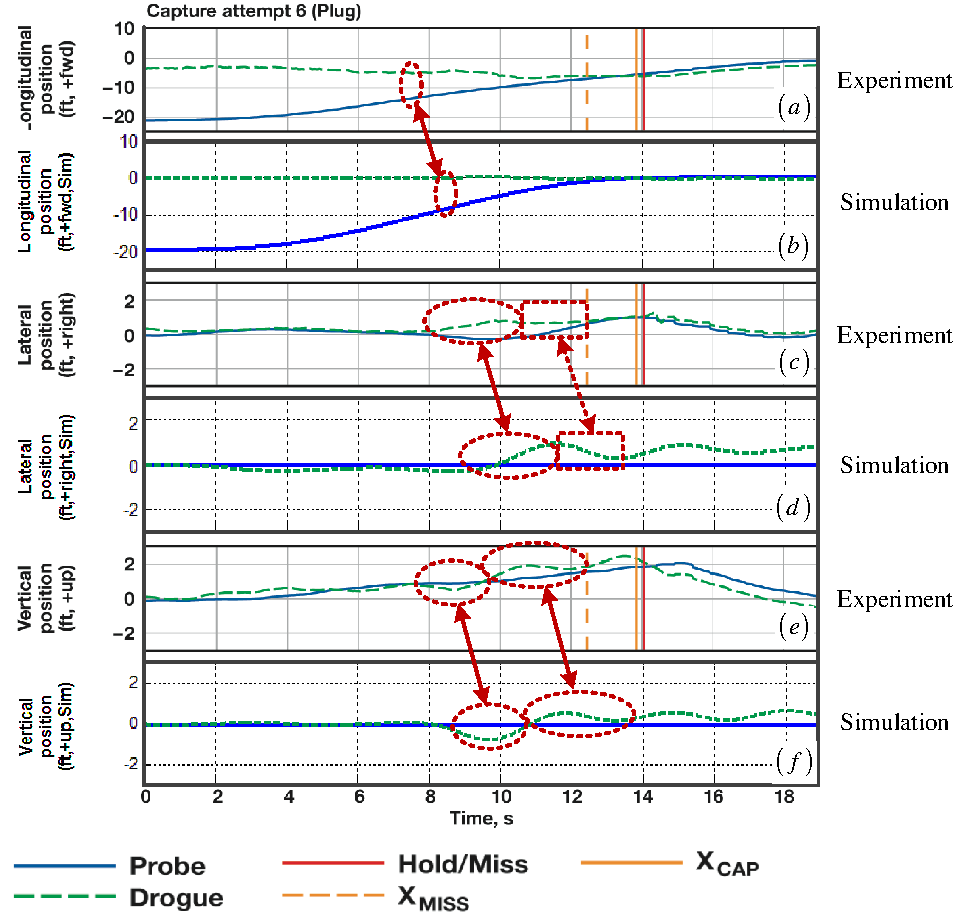
\includegraphics[width=0.6\textwidth]{Chap4/fig23.pdf}
%	\caption{Difference in Drogue Displacement with and without HDU}\label{fig4.23}
%\end{figure}
%
%In the absence of the HDU, the pendulum length remains unchanged, as shown in Fig. \ref{fig4.23}(a). Within the equilibrium range, applying a force to the endpoint of the pendulum, apart from the force direction normal to the equilibrium position, will result in a tangential motion of the pendulum due to forces acting in other directions. In a steady state, the hose tends to be in a more horizontal position, causing both ${F_{{\rm{b}}x}}$ and ${F_{{\rm{b}}z}}$ to primarily induce displacement of the drogue along the ${o_{\rm{t}}}{z_{\rm{t}}}$ direction. This also indicates a significant coupling of the drogue's dynamics in the absence of the HDU.
%When the HDU is considered, it adjusts the length of the exposed hose outside the aircraft in response to changes in hose tension, as depicted in Fig. \ref{fig4.23}(b). When the drogue experiences a longitudinal force ${F_{{\rm{b}}x}}$ from the bow wave, the HDU reduces the length of the exposed hose, thereby changing the primary direction of movement of the drogue from downward to forward. It is evident that the HDU modifies the dynamics of the drogue during the docking process.
%
%\subsection{Model of the HDU}
%
%The model of the HDU typically employs a reel model\cite{vassberg_numerical_2004}, and its dynamics can be expressed as follows 
%\begin{equation}\label{eq4.119}
%	\left( {{T_{{\rm{reel}}}} - {T_{{\rm{hose}}}}} \right){r_{{\rm{reel}}}} = {I_{{\rm{reel}}}}{\alpha _{{\rm{reel}}}}
%\end{equation}
%where ${T_{{\rm{reel}}}}$ and ${T_{{\rm{hose}}}}$ represent the tension in the reel and the tension at the upper end of the hose, respectively. Since the direction of force is not analyzed here, scalar magnitudes of tension are used. The symbols ${r_{{\rm{reel}}}}, {I_{{\rm{reel}}}}$ and ${\alpha _{{\rm{reel}}}}$ represent the radius of the reel, moment of inertia, and angular acceleration around its central axis. Furthermore, if the reel is considered as a cylindrical object, one have 
%\begin{equation}\label{eq4.120}
%	{I_{{\rm{reel}}}} = {m_{{\rm{reel}}}}r_{{\rm{reel}}}^2
%\end{equation}
%On the other hand, expressing ${\alpha _{{\rm{reel}}}}$ in terms of linear acceleration 
%\begin{equation}\label{eq4.121}
%	{\alpha _{{\rm{reel}}}} = \frac{{{{\ddot l}_1}}}{{{r_{{\rm{reel}}}}}}
%\end{equation}
%It should be noted that the change in the length of the hose is replaced by the change in the length of the first link. Although from Section 4.2 it can be understood that the one exposed is the $i$-th link, due to the relatively small retraction of the hose during the docking process, extending the original length of the first link appropriately ensures that the first link is always exposed. Of course, the model of variable first link in Section 4.2.5 can also be used, but it involves more complex calculations. Substituting Eqs. (\ref{eq4.120}) and (\ref{eq4.121}) into Eq. (\ref{eq4.119}), the kinematic model of HDU can be obtained as 
%\begin{equation}\label{eq4.122}
%	{\ddot l_1} = \frac{{{T_{{\rm{reel}}}} - {T_{{\rm{hose}}}}}}{{{m_{{\rm{reel}}}}}}
%\end{equation}
%The dynamic model of the HDU is determined by its controller, which will be elaborated on in the next section.
%
%\subsection{HDU Controller and Qualitative Analysis of its Control Effect}
%
%The controller of the HDU adjusts ${T_{{\rm{reel}}}}$ by using the state variables of the hose (such as ${T_{{\rm{hose}}}},{l_1}$ and ${\dot l_1}$) to indirectly control the length of the exposed hose, thereby regulating the hose tension and achieving equilibrium without causing hose whipping phenomenon. Fig. \ref{fig4.24} illustrates the structural diagram of the link-connected hose-drogue model with the inclusion of the HDU.
%
%(1)Two Types of Controllers for HDU
%
%The first type of controller is the one proposed in Refs. \cite{vassberg_numerical_2004,ro_modeling_2010}.
%\begin{equation}\label{eq4.123}
%	{T_{{\rm{reel}}}}\left( t \right) = {T_{{\rm{reel}}}}\left( 0 \right){\left[ {\frac{{{l_1}\left( t \right)}}{{{l_1}\left( 0 \right)}}} \right]^k},0 < {l_1}\left( t \right) \le {l_1}\left( 0 \right)
%\end{equation}
%That is, at $t = 0$, when the hose is just fully extended, ${T_{{\rm{reel}}}}\left( 0 \right)$ represents the tension at that moment, ${l_1}\left( 0 \right)$ is the length of the first link at that moment, and $k \in \mathbb{R}_{+}$ is the parameter of the controller. It can be observed from Eqs. (\ref{eq4.122}) and (\ref{eq4.123}) that when the hose is completely extended (which corresponds to the state at $t = 0$), the controller achieves equilibrium, and there is no change in the hose length.
%\begin{figure}[th]
%	\centering
%	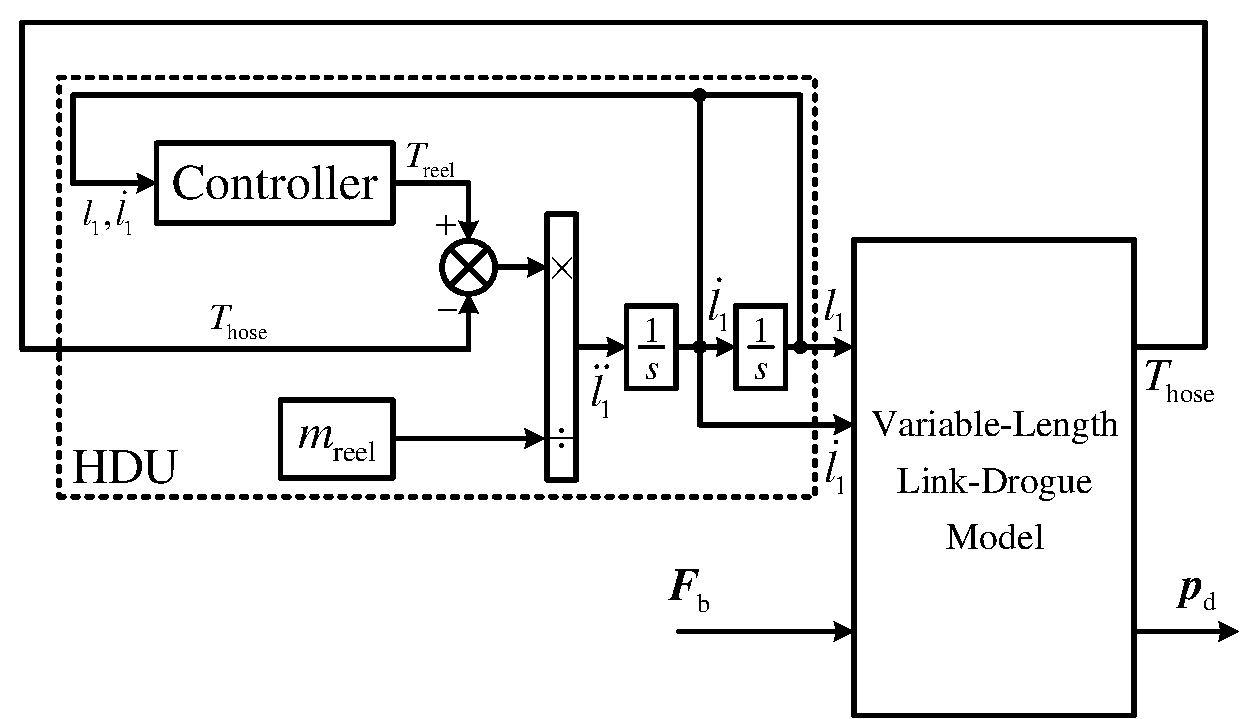
\includegraphics[width=0.7\textwidth]{Chap4/fig24.pdf}
%	\caption{Schematic of link-connected hose-drogue model with HDU}\label{fig4.24}
%\end{figure}
%While the first type of controller does regulate the hose tension, its transient behavior is suboptimal. Therefore, based on the first type of controller, the second type of controller is proposed 
%\begin{equation}\label{eq4.124}
%	{T_{{\rm{reel}}}}\left( t \right) = {T_{{\rm{reel}}}}\left( 0 \right){\left[ {\frac{{{l_1}\left( t \right)}}{{{l_1}\left( 0 \right)}}} \right]^k} + {k_d}{\dot l_1}\left( t \right),0 < {l_1}\left( t \right) \le {l_1}\left( 0 \right)
%\end{equation}
%where ${k_d} \in \mathbb{R}_{+}$. The second type of controller introduces a damping term ${k_d}{\dot l_1}\left( t \right)$, which can effectively improve the transient performance. Furthermore, since we can directly measure the linear velocity of the hose length change, or indirectly obtain the hose length change through the rotation speed of the drum, this controller is easy to implement.
%
%Next, the HDU and the variable-length link-connected hose-drogue model will be used to simulate the control effects of the two types of controllers and analyze the effects of different $k$ values on each type of controller.
%
%(2)Simulation and Qualitative Analysis of Two Types of Controllers
%
%Firstly, establish the simulation model as shown in Fig. \ref{fig4.24}. The basic settings of the simulation environment are outlined in Table \ref{tab4.2}. For the sake of convenience in simulation, some of the parameters listed in Table \ref{tab4.2} have been modified in this chapter's simulations. Additionally, new simulation parameters related to the HDU have been added, as depicted in Table \ref{tab4.3}.
%
%Let the force ${\bm {f}_{\rm{b}}}$ experience a step change from ${\left[ {\begin{array}{*{20}{c}}
%	0&0&0
%\end{array}} \right]^{\rm{T}}}$ to ${\left[ {\begin{array}{*{20}{c}}
%	{75}&0&0
%\end{array}} \right]^{\rm{T}}}$ at 100 seconds. This is done to mimic the force difference in the ${o_{\rm{t}}}{x_{\rm{t}}}$ direction that contributed to the disparities between simulations and experiments in Section 4.3.4. For both the first type of controller and the second type of controller, select the controller parameters as $k = \left\{ {0.3,0.5,1,3} \right\}$, with ${k_d} = 500$ for the second type of controller.
%
%The simulation results are presented in Fig. \ref{fig4.25}. Subfigures (a1)-(a4) depict the control effects of the first type of controller, while subfigures (b1)-(b4) illustrate the control effects of the second type of controller. Through comparison, the following conclusions can be qualitatively drawn:
%
%1) Comparing subfigures (a1)-(a4) and (b1)-(b4) in Fig. \ref{fig4.25}, it can be observed that the first type of controller leads to pronounced oscillations with a longer settling time. In contrast, the second type of controller exhibits significant improvements in both tension adjustment and drogue position control, showing smoother transition dynamics than the first type of controller.
%
%2) Comparing Fig. \ref{fig4.25} (a1) with Fig. \ref{fig4.25} (b1), it can be deduced that the parameter $k$ does not influence the steady-state value of the final hose tension.
%
%3) Comparing Fig. \ref{fig4.25} (a1) with Fig. \ref{fig4.25} (b1), it can be observed that the parameter $k$ significantly affects the retraction length of the hose. When $k$ is smaller, the HDU needs to retract a longer length of the hose to achieve the same steady-state tension value. Conversely, if a minimal change in hose length is desired, a larger $k$ value can be chosen.
%
%4) A larger value of $k$ brings about a noticeable negative effect, which makes the HDU-hose-drogue system unstable. This can be observed from Figs. \ref{fig4.25} (a1)-(a4), where the adjustment time of various quantities significantly increases with the increase in $k$. In fact, for the first type of controller with $k = 4$, the outputs of various quantities have already diverged. In contrast, comparing Figs. \ref{fig4.25} (b1)-(b4) reveals that the second type of controller shows significant improvement in addressing this phenomenon.
%
%5) From Figs. \ref{fig4.25} (a3) and (a4) and Figs \ref{fig4.25} (b3) and (b4), it can be observed that the parameter $k$ indirectly influences the dynamics of the drogue in various directions by affecting the length of the hose. This characteristic will be further discussed in the subsequent sections of this chapter.
%
%% Table generated by Excel2LaTeX from sheet 'Sheet1'
%\begin{table}[htbp]
%	\centering
%	\caption{Parameters Used in HDU Simulation}
%	  \begin{tabular}{|l|c|c|}
%		\hline Parameters    & Values & Units \\ \hline
%		Number of Link Segments $N$  & $10$    & - \\ \hline
%		Initial Length of the First Link ${l_1}\left( 0 \right)$ & $2$     & $m$ \\ \hline
%		Lengths of the Remaining Links ${l_j}\left( 0 \right),j = 2,3, \ldots ,N$ & $13/9$  & $m$ \\ \hline
%		The Mass of the Reel ${m_{{\rm{reel}}}}$& $68$    & $kg$ \\ \hline
%		Initial Tension of the Reel  & 1610  & $N$ \\ \hline
%	  \end{tabular}%
%	\label{tab4.4}%
%\end{table}%
%\begin{figure}[th]
%	\centering
%	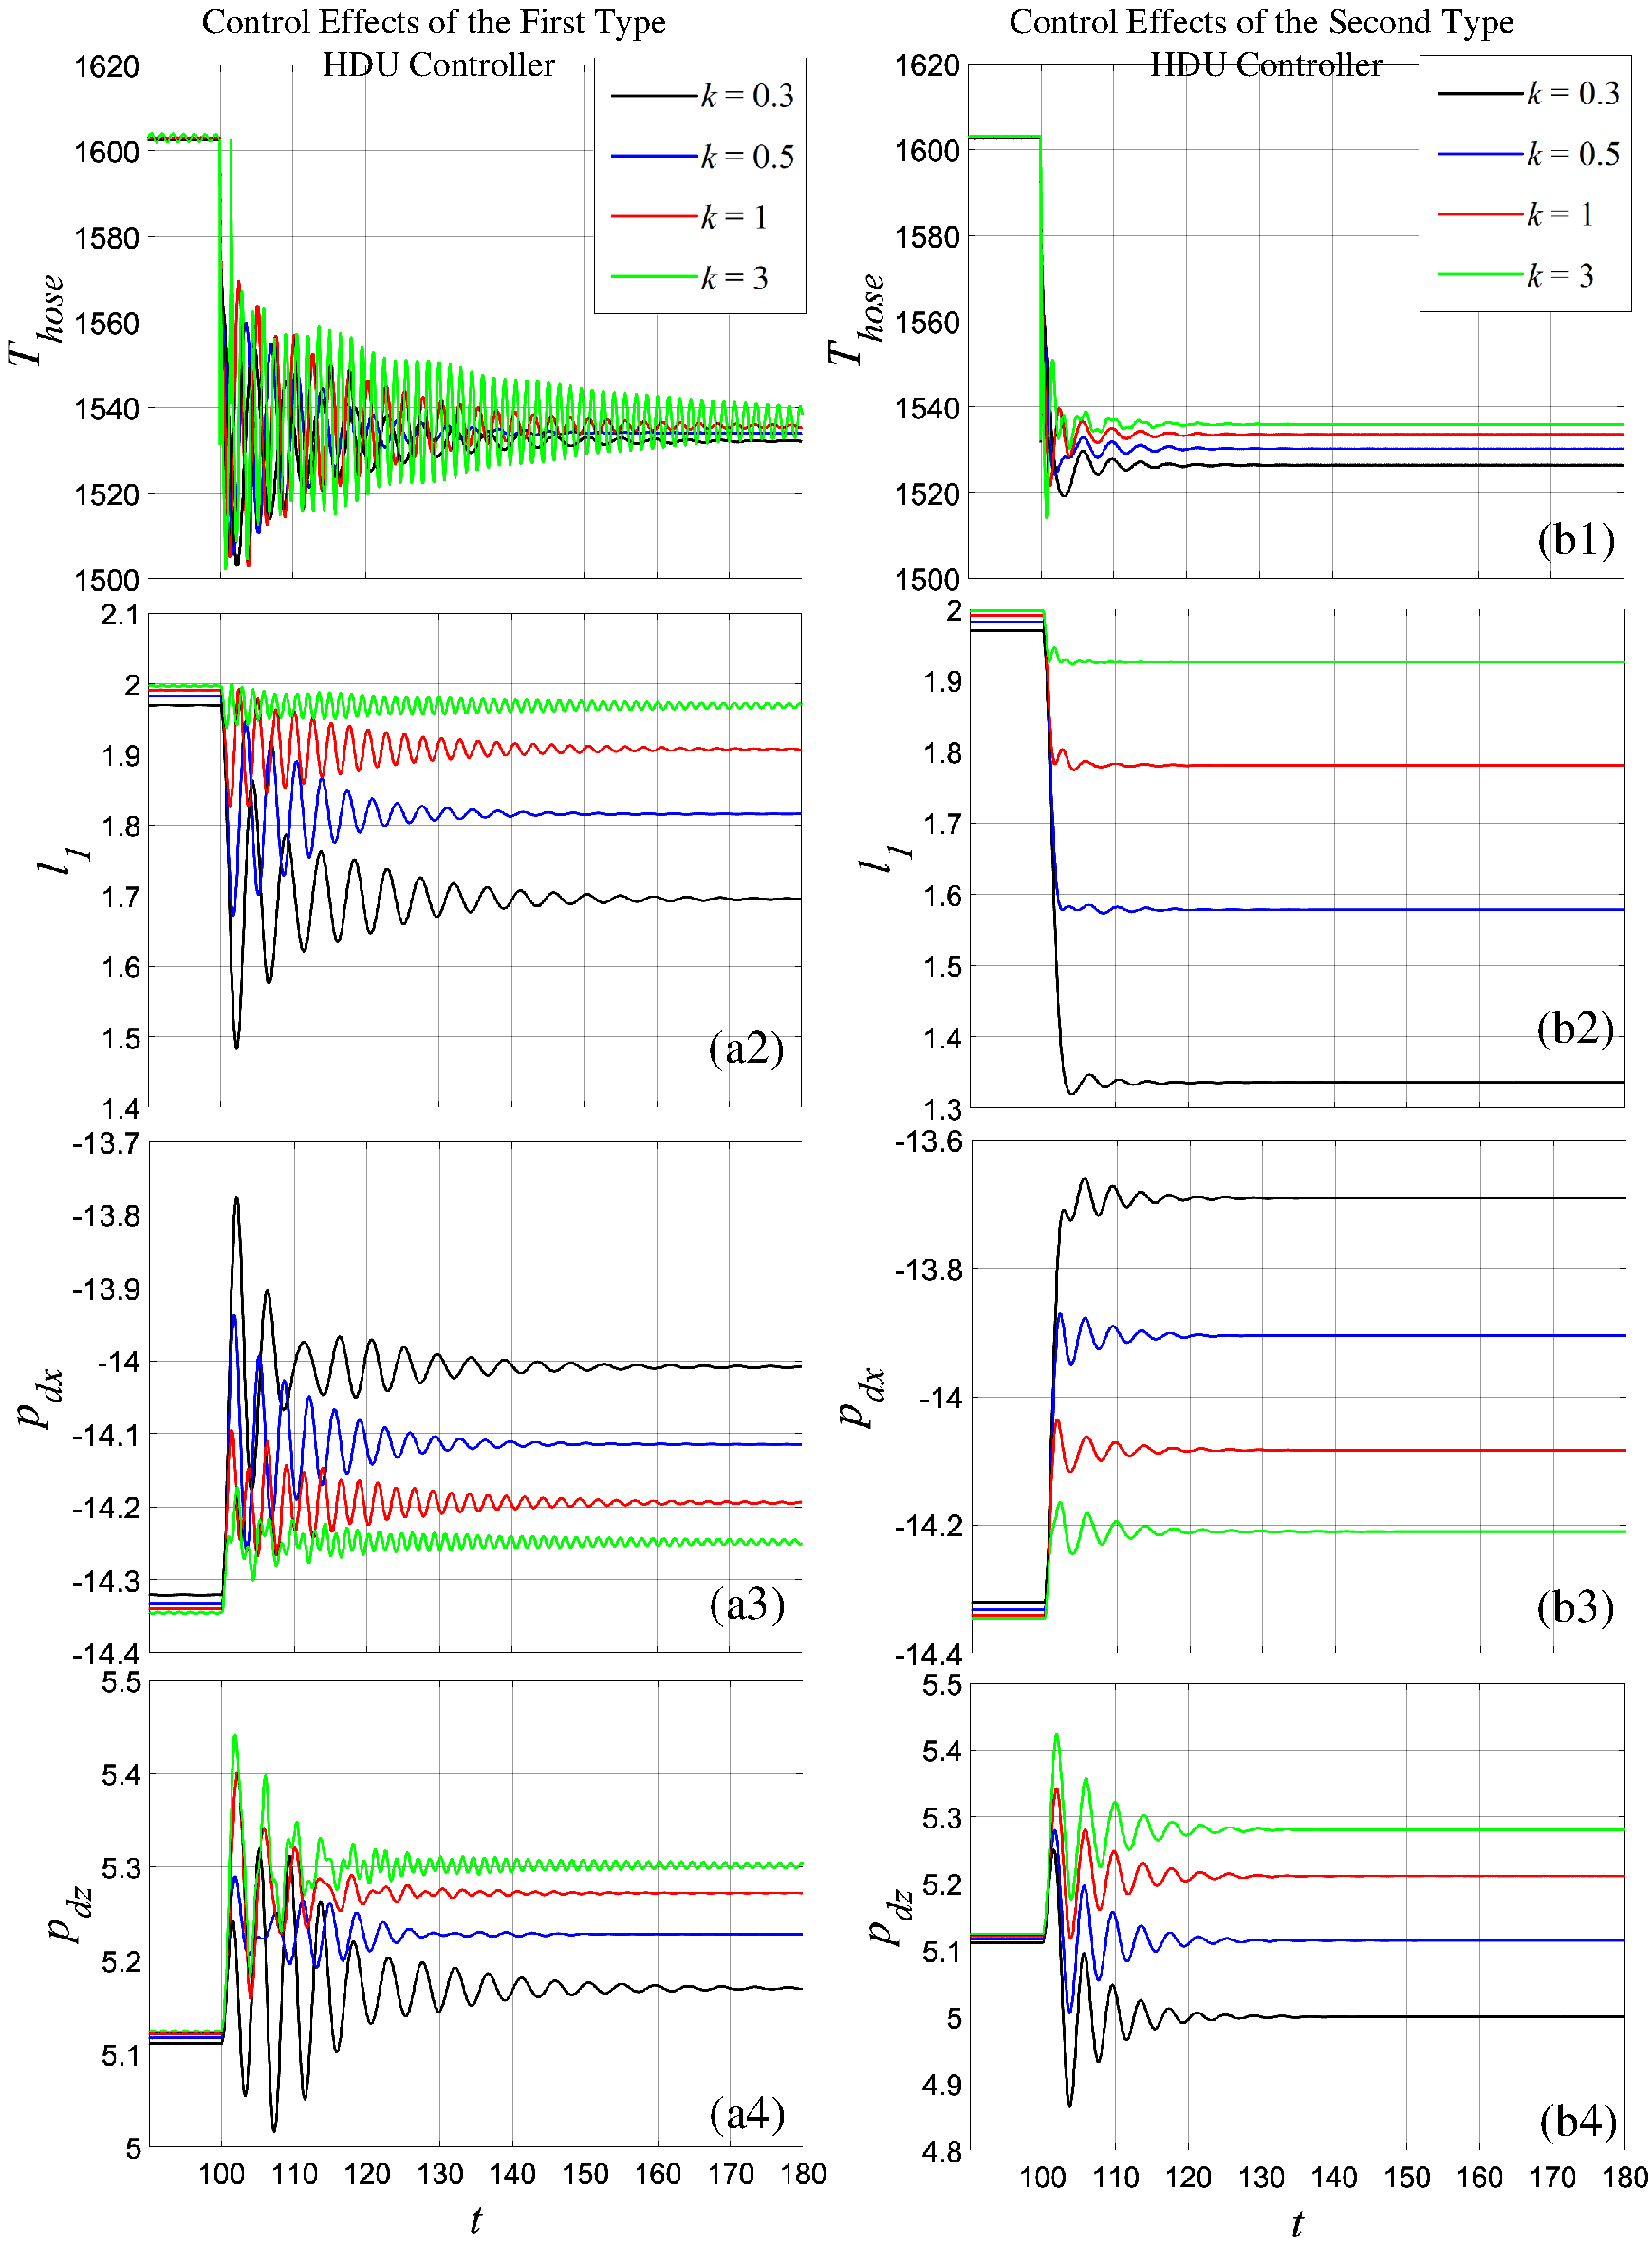
\includegraphics[width=0.7\textwidth]{Chap4/fig25.pdf}
%	\caption{Control Effects of Two Types of HDU Controllers}\label{fig4.25}
%\end{figure} 
%\section{Simplified Drogue Dynamic Model}
%
%Regardless of whether the link-connected hose-drogue model includes the HDU, the model is too complex. As described in Section 4.2, to better simulate the dynamics of the hose, a significant number of links are required, with each link having multiple state variables such as ${\alpha _j},{\beta _j},{\dot \alpha _j},{\dot \beta _j},{l_j},{\dot l_j}$, etc. This complexity results in a high-order link-connected hose-drogue model. Additionally, the presence of nonlinear operations in model calculations further increases its complexity. However, when designing a docking controller, only the dynamics of the drogue are concerned with, and the dynamics of other links become redundant. Therefore, this section aims to simplify the link-connected hose-drogue model in order to obtain a model that solely expresses the dynamics of the drogue. This simplified model is referred to as the drogue dynamics model. It has a lower order and is suitable for controller design in subsequent chapters. Furthermore, it allows for quantitative analysis of the drogue's dynamics under different HDU models.
%
%\subsection{Problem Description and Modeling Approach for Drogue Dynamic Model}
%
%(1) Problem Description for Drogue Dynamic Model
%
%In Section 4.3.1, the link-connected hose-drogue model was represented using Eq. (\ref{eq4.99}). If taking the HDU model into account, with the drogue's forces as inputs and the drogue's position as output, the system can be expressed as follows 
%\begin{equation}\label{eq4.125}
%	\left\{ \begin{aligned}
%		&{{ {\dot {\bf{x}}}}_{{\rm{reel}}}} = { {{\bm{f}}}_{{\rm{reel}}}}\left( {{ {{\bf{x}}}_{{\rm{reel}}}},{ {{\bf{x}}}_{\rm{h}}}} \right)\\
%		&{{ {\dot {\bf{x}}}}_{\rm{h}}} = { {{\bm{f}}}_{{\rm{h0}}}}\left( {{ {{\bf{x}}}_{\rm{h}}},{ {{\bf{x}}}_{\rm{d}}}, {{\mathbf{v}}}_{{\rm{t/w}}}^{\rm{g}},h_{\rm{t}}^{\rm{g}}} \right)\\
%		&{{ {\dot {\bm{x}}}}_{\rm{d}}} = { {{\bm{f}}}_{{\rm{d0}}}}\left( {{ {{\bm{x}}}_{\rm{h}}},{ {{\bf{x}}}_{\rm{d}}}, {{\mathbf{v}}}_{{\rm{t/w}}}^{\rm{g}},h_{\rm{t}}^{\rm{g}},{ {{\bf{F}}}_{\rm{b}}}} \right)\\
%		&{ {{\bf{p}}}_{\rm{d}}} = { {{\bm{f}}}_y}\left( {{ {{\bf{x}}}_{\rm{h}}},{ {{\bf{x}}}_{\rm{d}}}} \right)
%		\end{aligned} \right.
%\end{equation}
%where ${ {{\bf{x}}}_{{\rm{reel}}}}$ represents the state variables of the HDU, and ${ {{\bm{f}}}_{{\rm{reel}}}}$ represents the function related to the dynamics of the HDU as described in Section 4.4. Under a constant tanker altitude ${h_0}$ and airspeed ${ \bm{v}_0}$, the model is simplified to 
%\begin{equation}\label{eq4.126}
%	\left\{ \begin{aligned}
%		&{{ {\dot {\bf{x}}}}_{{\rm{reel}}}} = { {{\bm{f}}}_{{\rm{reel}}}}\left( {{ {{\bf{x}}}_{{\rm{reel}}}},{ {{\bf{x}}}_{\rm{h}}}} \right)\\
%		&{{ {\dot {\bf{x}}}}_{\rm{h}}} = { {{\bm{f}}}_{\rm{h}}}\left( {{ {{\bf{x}}}_{{\rm{reel}}}},{ {{\bf{x}}}_{\rm{h}}},{ {{\bf{x}}}_{\rm{d}}}} \right)\\
%		&{{ {\dot {\bf{x}}}}_{\rm{d}}} = { {{\bm{f}}}_{\rm{d}}}\left( {{ {{\bm{x}}}_{\rm{h}}},{ {{\bf{x}}}_{\rm{d}}},{ {{\mathbf{F}}}_{\rm{b}}}} \right)\\
%		&{ {{\bf{p}}}_{\rm{d}}} = { {{\bm{f}}}_y}\left( {{ {{\bf{x}}}_{\rm{h}}},{ {{\bf{x}}}_{\rm{d}}}} \right)
%		\end{aligned} \right.
%\end{equation}
%where ${ {{\bm{f}}}_{\rm{h}}}\left( {{ {{\bf{x}}}_{\rm{h}}},{ {{\bf{x}}}_{\rm{d}}}} \right) \triangleq { {{\bm{f}}}_{{\rm{h0}}}}\left( {{ {{\bf{x}}}_{\rm{h}}},{ {{\bf{x}}}_{\rm{d}}},{ {{\bf{v}}}_0},{h_0}} \right),{ {{\bm{f}}}_{\rm{d}}}\left( {{ {{\bf{x}}}_{\rm{h}}},{ {{\bf{x}}}_{\rm{d}}},{ {{\bf{F}}}_{\rm{b}}}} \right) \triangleq { {{\bm{f}}}_{{\rm{d0}}}}\left( {{ {{\bf{x}}}_{\rm{h}}},{ {{\bf{x}}}_{\rm{d}}},{ {{\bf{v}}}_0},{h_0},{ {{\bf{F}}}_{\rm{b}}}} \right)$. Then, for each set of $\left( {{ {{\bf{v}}}_0},{h_0}} \right)$, and when the system (\ref{eq4.126}) is subjected to zero input (i.e., ${ {{\bf{F}}}_{\rm{b}}} = {\bf{0}}$), the system will reach a steady-state position. Denote the state of the system at this time as the equilibrium state 
%\begin{equation}\label{eq4.127}
%	{ {{\bf{x}}}_{{\rm{reel}}}} =  {{\bf{x}}}_{{\rm{reel}}}^*,{ {{\bf{x}}}_{\rm{h}}} =  {{\bf{x}}}_{\rm{h}}^{\rm{*}},{ {{\bf{x}}}_{\rm{d}}} =  {{\bf{x}}}_{\rm{d}}^{\rm{*}}
%\end{equation}
%At this moment, the system satisfies the equation 
%\begin{equation}\label{eq4.128}
%	\left\{ \begin{aligned}
%		 &{\dot {\bf{x}}}_{{\rm{reel}}}^* = { {{\bm{f}}}_{{\rm{reel}}}}\left( { {{\bf{x}}}_{{\rm{reel}}}^*, {{\bf{x}}}_{\rm{h}}^{\rm{*}}} \right)\\
%		 &{\dot {\bf{x}}}_{\rm{h}}^{\rm{*}} = { {{\bm{f}}}_{\rm{h}}}\left( { {{\bf{x}}}_{{\rm{reel}}}^*, {{\bf{x}}}_{\rm{h}}^{\rm{*}}, {{\bf{x}}}_{\rm{d}}^{\rm{*}}} \right)\\
%		 &{\dot {\bf{x}}}_{\rm{d}}^{\rm{*}} = { {{\bm{f}}}_{\rm{d}}}\left( { {{\bf{x}}}_{\rm{h}}^{\rm{*}}, {{\bf{x}}}_{\rm{d}}^{\rm{*}},{\bf{0}}} \right)\\
%		 &{{\bf{p}}}_{\rm{d}}^{\rm{*}} = { {{\bm{f}}}_y}\left( { {{\bf{x}}}_{\rm{h}}^{\rm{*}}, {{\bf{x}}}_{\rm{d}}^{\rm{*}}} \right)
%		\end{aligned} \right.
%\end{equation}
%Linearizing the system (\ref{eq4.126}) at the equilibrium point (\ref{eq4.128}), we can obtain 
%\begin{equation}\label{eq4.129}
%	\left\{ \begin{aligned}
%		\left[ {\begin{array}{*{20}{c}}
%		{\Delta {{ {\dot {\bf{x}}}}_{{\rm{reel}}}}}\\
%		{\Delta {{ {\dot {\bf{x}}}}_{\rm{h}}}}\\
%		{\Delta {{ {\dot {\bf{x}}}}_{\rm{d}}}}
%		\end{array}} \right] &= \underbrace {\left[ {\begin{array}{*{20}{c}}
%		{{{\bf{A}}_{11}}}&{{{\bf{A}}_{12}}}&{\bf{0}}\\
%		{{{\bf{A}}_{21}}}&{{{\bf{A}}_{22}}}&{{{\bf{A}}_{23}}}\\
%		{\bf{0}}&{{{\bf{A}}_{32}}}&{{{\bf{A}}_{33}}}
%		\end{array}} \right]}_{\bf{A}}\left[ {\begin{array}{*{20}{c}}
%		{\Delta { {{\bf{x}}}_{{\rm{reel}}}}}\\
%		{\Delta { {{\bf{x}}}_{\rm{h}}}}\\
%		{\Delta { {{\bf{x}}}_{\rm{d}}}}
%		\end{array}} \right] + \underbrace {\left[ {\begin{array}{*{20}{c}}
%		{\bf{0}}\\
%		{\bf{0}}\\
%		{{{\bf{B}}_3}}
%		\end{array}} \right]}_{\bf{B}}{\bf {F}_{\rm{b}}}{\rm{ + }}\left[ {\begin{array}{*{20}{l}}
%		{o\left( {\Delta { {{\bm{x}}}_{{\rm{reel}}}},\Delta { {{\bf{x}}}_{\rm{h}}}} \right)}\\
%		{o\left( {\Delta { {{\bm{x}}}_{{\rm{reel}}}},\Delta { {{\bf{x}}}_{\rm{h}}},\Delta { {{\bm{x}}}_{\rm{d}}}} \right)}\\
%		{o\left( {\Delta { {{\bm{x}}}_{\rm{h}}},\Delta { {{\bf{x}}}_{\rm{d}}},{ {F}_{\rm{b}}}} \right)}
%		\end{array}} \right]\\
%		\Delta { {{\bf{p}}}_{\rm{d}}} &= \underbrace {\left[ {\begin{array}{*{20}{c}}
%		{\bf{0}}&{{{\bf{C}}_2}}&{{{\bf{C}}_3}}
%		\end{array}} \right]}_{\bf{C}}\left[ {\begin{array}{*{20}{c}}
%		{\Delta { {{\bf{x}}}_{{\rm{reel}}}}}\\
%		{\Delta { {{\bf{x}}}_{\rm{h}}}}\\
%		{\Delta { {{\bf{x}}}_{\rm{d}}}}
%		\end{array}} \right] + o\left( {\Delta { {{\bf{x}}}_{\rm{h}}},\Delta { {{\bf{x}}}_{\rm{d}}}} \right)
%		\end{aligned} \right.
%\end{equation}
%where
%\begin{equation}\label{eq4.130}
%	\begin{array}{*{20}{l}}
%		{{{\bf{A}}_{11}}{\rm{ = }}{{\left. {\frac{{\partial { {{\bm{f}}}_{{\rm{reel}}}}}}{{\partial { {{\bf{x}}}_{{\rm{reel}}}}}}} \right|}_{\scriptstyle{ {{\bf{x}}}_{{\rm{reel}}}} =  {{\bf{x}}}_{{\rm{reel}}}^*\hfill\atop
%		\scriptstyle{ {{\bf{x}}}_{\rm{h}}} =  {{\bf{x}}}_{\rm{h}}^{\rm{*}}\hfill}},}&{{{\bf{A}}_{12}}{\rm{ = }}{{\left. {\frac{{\partial { {{\bm{f}}}_{{\rm{reel}}}}}}{{\partial { {{\bf{x}}}_{\rm{h}}}}}} \right|}_{\scriptstyle{ {{\bf{x}}}_{{\rm{reel}}}} =  {{\bf{x}}}_{{\rm{reel}}}^*\hfill\atop
%		\scriptstyle{ {{\bf{x}}}_{\rm{h}}} =  {{\bf{x}}}_{\rm{h}}^{\rm{*}}\hfill}},}&{{{\bf{A}}_{21}}{\rm{ = }}{{\left. {\frac{{\partial { {{\bm{f}}}_{\rm{h}}}}}{{\partial { {{\bf{x}}}_{{\rm{reel}}}}}}} \right|}_{\scriptstyle{ {{\bf{x}}}_{{\rm{reel}}}} =  {{\bf{x}}}_{{\rm{reel}}}^*\hfill\atop
%		{\scriptstyle{ {{\bf{x}}}_{\rm{h}}} =  {{\bf{x}}}_{\rm{h}}^{\rm{*}}\hfill\atop
%		\scriptstyle{ {{\bf{x}}}_{\rm{d}}} =  {{\bf{x}}}_{\rm{d}}^{\rm{*}}\hfill}}},}&{{{\bf{A}}_{22}}{\rm{ = }}{{\left. {\frac{{\partial { {{\bm{f}}}_{\rm{h}}}}}{{\partial { {{\bf{x}}}_{\rm{h}}}}}} \right|}_{\scriptstyle{ {{\bf{x}}}_{{\rm{reel}}}} =  {{\bf{x}}}_{{\rm{reel}}}^*\hfill\atop
%		{\scriptstyle{ {{\bf{x}}}_{\rm{h}}} =  {{\bf{x}}}_{\rm{h}}^{\rm{*}}\hfill\atop
%		\scriptstyle{ {{\bf{x}}}_{\rm{d}}} =  {{\bf{x}}}_{\rm{d}}^{\rm{*}}\hfill}}},}\\
%		{{{\bf{A}}_{23}}{\rm{ = }}{{\left. {\frac{{\partial { {f}_{\rm{h}}}}}{{\partial { {{\bf{x}}}_{\rm{d}}}}}} \right|}_{\scriptstyle{ {{\bf{x}}}_{{\rm{reel}}}} =  {{\bf{x}}}_{{\rm{reel}}}^*\hfill\atop
%		{\scriptstyle{ {{\bf{x}}}_{\rm{h}}} =  {{\bf{x}}}_{\rm{h}}^{\rm{*}}\hfill\atop
%		\scriptstyle{ {{\bf{x}}}_{\rm{d}}} =  {{\bf{x}}}_{\rm{d}}^{\rm{*}}\hfill}}},}&{{{\bf{A}}_{32}}{\rm{ = }}{{\left. {\frac{{\partial { {{\bm{f}}}_{\rm{d}}}}}{{\partial { {{\bf{x}}}_{\rm{h}}}}}} \right|}_{\scriptstyle{ {{\bf{x}}}_{\rm{h}}} =  {{\bf{x}}}_{\rm{h}}^{\rm{*}}\hfill\atop
%		{\scriptstyle{ {{\bf{x}}}_{\rm{d}}} =  {{\bf{x}}}_{\rm{d}}^{\rm{*}}\hfill\atop
%		\scriptstyle{ {F}_{\rm{b}}} = 0\hfill}}},}&{{{\bf{A}}_{33}}{\rm{ = }}{{\left. {\frac{{\partial { {{\bm{f}}}_{\rm{d}}}}}{{\partial { {{\bf{x}}}_{\rm{d}}}}}} \right|}_{\scriptstyle{ {{\bf{x}}}_{\rm{h}}} =  {{\bf{x}}}_{\rm{h}}^{\rm{*}}\hfill\atop
%		{\scriptstyle{ {{\bf{x}}}_{\rm{d}}} =  {{\bf{x}}}_{\rm{d}}^{\rm{*}}\hfill\atop
%		\scriptstyle{ {F}_{\rm{b}}} = 0\hfill}}},}&{{{\bf{B}}_3}{\rm{ = }}{{\left. {\frac{{\partial { {{\bm{f}}}_{\rm{d}}}}}{{\partial { {{\bm{f}}}_{\rm{b}}}}}} \right|}_{\scriptstyle{ {{\bf{x}}}_{\rm{h}}} =  {{\bf{x}}}_{\rm{h}}^{\rm{*}}\hfill\atop
%		{\scriptstyle{ {{\bf{x}}}_{\rm{d}}} =  {{\bf{x}}}_{\rm{d}}^{\rm{*}}\hfill\atop
%		\scriptstyle{ {F}_{\rm{b}}} = 0\hfill}}},}\\
%		{{{\bf{C}}_2}{\rm{ = }}{{\left. {\frac{{\partial { {{\bm{f}}}_y}}}{{\partial { {{\bf{x}}}_{\rm{h}}}}}} \right|}_{\scriptstyle{ {{\bf{x}}}_{\rm{h}}} =  {{\bf{x}}}_{\rm{h}}^{\rm{*}}\hfill\atop
%		\scriptstyle{ {{\bf{x}}}_{\rm{d}}} =  {{\bf{x}}}_{\rm{d}}^{\rm{*}}\hfill}},}&{{{\bf{C}}_3}{\rm{ = }}{{\left. {\frac{{\partial { {{\bm{f}}}_y}}}{{\partial { {{\bf{x}}}_{\rm{d}}}}}} \right|}_{\scriptstyle{ {{\bf{x}}}_{\rm{h}}} =  {{\bf{x}}}_{\rm{h}}^{\rm{*}}\hfill\atop
%		\scriptstyle{ {{\bf{x}}}_{\rm{d}}} =  {{\bf{x}}}_{\rm{d}}^{\rm{*}}\hfill}}}&{}&{}
%		\end{array}
%\end{equation}
%and $\Delta { {{\bf{x}}}_{{\rm{reel}}}} = { {{\bf{x}}}_{{\rm{reel}}}} -  {{\bf{x}}}_{{\rm{reel}}}^*,\Delta { {{\bf{x}}}_{\rm{h}}} = { {{\bf{x}}}_{\rm{h}}} -  {{\bf{x}}}_{\rm{h}}^*,\Delta { {{\bf{x}}}_{\rm{d}}} = { {{\bf{x}}}_{\rm{d}}} -  {{\bf{x}}}_{\rm{d}}^*,\Delta { {{\bf{p}}}_{\rm{d}}} = { {{\bf{p}}}_{\rm{d}}} -  {{\bf{p}}}_{\rm{d}}^{\rm{*}}$, according to the drogue equilibrium coordinate system, it can be observed that $\Delta { {{\bf{p}}}_{\rm{d}}} =  {{\bf{p}}}_{\rm{d}}^{\rm{e}}$, and $o(\cdot)$ represents higher-order infinitesimal terms in the linearization. Since the changes in the state of the hose and the drogue are relatively small during the docking process, i.e., $\Delta { {{\bf{x}}}_{{\rm{reel}}}},\Delta { {{\bf{x}}}_{\rm{h}}}$ and $\Delta { {{\bf{x}}}_{\rm{d}}}$ are infinitesimal terms that can be neglected. Additionally, if the subsequent model simplification can be validated through the process described in section 4.5.4, it would also indicate the reasonableness of omitting infinitesimal terms here. After neglecting infinitesimal terms, the system (\ref{eq4.129}) becomes a linear system. Subsequently, through Laplace transformation, the transfer function of this linear system can be expressed as 
%\begin{equation}\label{eq4.131}
%	 {{\bf{p}}}_{\rm{d}}^{\rm{e}}\left( s \right) = \underbrace {{\bf{C}}{{\left( {s{\bf{I}} - {\bf{A}}} \right)}^{ - 1}}{\bf{B}}}_{{{\bf{G}}_{\rm{d}}}\left( s \right)}{ {{\bf{F}}}_{\rm{b}}}\left( s \right)
%\end{equation}
%This equation is commonly referred to as the drogue dynamic model.
%
%(2) Modeling Approach for Drogue Dynamic Model
%
%The model (\ref{eq4.131}) includes ${{\bf{G}}_{\rm{d}}}\left( s \right)$, which represents the drogue's dynamics. Next, system identification methods will be used to obtain ${{\bf{G}}_{\rm{d}}}\left( s \right)$, and the following steps outline this process:
%
%1) Utilize axial force to infer the coupling relationships among different channels, and then obtain the basic form of ${{\bf{G}}_{\rm{d}}}\left( s \right)$.
%
%2) Employ Generalized Binary Noise (GBN) as an input to excite the system and identify system parameters.
%
%3) Validate the identified results using a Chirp Signal.
%
%In Sections 4.5.2-4.5.4, we will combine an example of a fixed-length link-connected model to explain the above process. The object to be identified in this example is the same as the one in Section 4.2.5. The obtained drogue dynamic model can be analyzed and compared with the later derived link-connected hose-drogue model with HDU.
%
%\subsection{Speculation on the Form of ${{\bf{G}}_{\rm{d}}}\left( s \right)$}
%
%Five simulations are conducted, each applying an axial force in a different direction to ${\bf{F}_{\rm{b}}}$. The forces were as follows  ${\bf{F}_{{\rm{b}}x{\rm{ + }}}} = {\left[ {\begin{array}{*{20}{c}}
%	{50}&0&0
%\end{array}} \right]^{\rm{T}}}$, ${\bf{F}_{{\rm{b}}y{\rm{ + }}}} = {\left[ {\begin{array}{*{20}{c}}
%		0&{50}&0
%\end{array}} \right]^{\rm{T}}}$, ${\bf{F}_{{\rm{b}}y - }} = {\left[ {\begin{array}{*{20}{c}}
%			0&{ - 50}&0
%\end{array}} \right]^{\rm{T}}}$, ${\bf{F}_{{\rm{b}}z{\rm{ + }}}} = {\left[ {\begin{array}{*{20}{c}}
%				0&0&{50}
%\end{array}} \right]^{\rm{T}}}$, ${\bf{F}_{{\rm{b}}z{\rm{ + }}}} = {\left[ {\begin{array}{*{20}{c}}
%					0&0&{ - 50}
%\end{array}} \right]^{\rm{T}}}$. The reason for not using forces in the ${\bf{F}_{{\rm{b}}x - }}$ direction for simulation is that, under normal circumstances, the receiver does not generate disturbances in the negative direction against the drogue. The choice of an amplitude of $50 N$ is because the maximum bow wave effect during the docking process is around $100 N$, and $50 N$ serves as a representative intermediate value for the bow wave effect. The results of these five simulations are presented in Table \ref{tab4.4}. In the table, $(\cdot)_\text{max}$ represents the maximum drift position of the drogue in the current simulation, while $(\cdot)_\text{final}$ represents the final drift position of the drogue in the current simulation.
%
%According to Table \ref{tab4.4}, the following conclusions can be drawn: 1) The $x$ and $z$ channels are coupled. 2) It can be assumed that the $y$ channel is decoupled from $x$ and $z$ channels, as the effects of ${\bf{F}_{{\rm{b}}y{\rm{ + }}}}$ and ${\bf{F}_{{\rm{b}}y - }}$ on ${x_{{d /t}}}$ and ${z_{{d /t}}}$ are much smaller than the forces in other directions. Therefore, the basic form of ${{\bf{G}}_{\rm{d}}}\left( s \right)$ can be obtained as follows 
%\begin{equation}\label{eq4.132}
%	{{\bf{G}}_{\rm{d}}}\left( s \right) = \left[ {\begin{array}{*{20}{c}}
%		{{G_{xx}}\left( s \right)}&0&{{G_{xz}}\left( s \right)}\\
%		0&{{G_{yy}}\left( s \right)}&0\\
%		{{G_{zx}}\left( s \right)}&0&{{G_{zz}}\left( s \right)}
%		\end{array}} \right]
%\end{equation}
%Additionally, in Section 4.2.5, it has been mentioned that the inherent dynamics of the drogue are of second order. Therefore, it can be inferred that the elements within ${{\bf{G}}_{\rm{d}}}\left( s \right)$ are also of second order.
%% Table generated by Excel2LaTeX from sheet 'Sheet1'
%\begin{table}[htbp]
%	\centering
%	\caption{Drift positions of the drogue under the influence of Fb in different directions}
%	  \begin{tabular}{|c|c|c|c|c|c|}
%		\hline \diagbox{${\bm{p}_{{d /t}}}$}{${\bf{F}_{\rm{b}}}$}& ${\bf{F}_{{\rm{b}}x{\rm{ + }}}}$ & ${\bf{F}_{{\rm{b}}y{\rm{ + }}}}$ &   ${\bf{F}_{{\rm{b}}y - }}$    &   ${\bf{F}_{{\rm{b}}z{\rm{ + }}}}$    & ${\bf{F}_{{\rm{b}}z - }}$ \\\hline
%			${\left( {{x_{{d /t}}}} \right)_{\max }}$& 0.07  & 0.015 & 0.015 & 0.204 & 0.177 \\\hline
%			${\left( {{x_{{d/t}}}} \right)_{{\rm{final}}}}$& 0.04  & 0.005 & 0.005 & 0.109 & 0.105 \\\hline
%			${\left( {{y_{{d/t}}}} \right)_{\max }}$& 0     & 0.724 & -0.724 & 0     & 0 \\\hline
%			${\left( {{y_{{d / t}}}} \right)_{{\rm{final}}}}$& 0     & 0.41  & -0.41 & 0     & 0 \\\hline
%			${\left( {{z_{{d/ t}}}} \right)_{\max }}$& 0.199 & -0.012 & -0.012 & 0.56  & -0.588 \\\hline
%			${\left( {{z_{{d / t}}}} \right)_{{\rm{final}}}}$& 0.115 & -0.004 & -0.004 & 0.324 & -0.447 \\\hline
%	  \end{tabular}%
%	\label{tab4.5}%
%\end{table}%
%  
%\subsection{System identification of the link-connected hose-drogue model}
%
%Using a GBN (Generalized Binary Noise) signal with an amplitude of $50 N$ to excite the system, as shown in Fig. \ref{fig4.26}, the parameters within ${{\bf{G}}_{\rm{d}}}\left( s \right)$ are identified using the Output-Error (OE) model \cite{ljung_system_1998}. The results can be obtained as follows 
%\begin{equation}\label{eq4.133}
%	\left\{ \begin{array}{c}
%		{G_{xx}}\left( s \right){\rm{ = }}\frac{{{\rm{0}}{\rm{.002185}}}}{{{s^2} + {\rm{0}}{\rm{.3071}}s + {\rm{2}}{\rm{.682}}}}\\
%		{G_{xz}}\left( s \right){\rm{ = }}\frac{{{\rm{0}}{\rm{.006169}}}}{{{s^2} + {\rm{0}}{\rm{.3013}}s + {\rm{2}}{\rm{.689}}}}\\
%		{G_{yy}}\left( s \right){\rm{ = }}\frac{{{\rm{0}}{\rm{.01712}}}}{{{s^2} + {\rm{0}}{\rm{.2422}}s + {\rm{2}}{\rm{.081}}}}\\
%		{G_{zx}}\left( s \right){\rm{ = }}\frac{{{\rm{0}}{\rm{.005824}}}}{{{s^2} + {\rm{0}}{\rm{.3223}}s + {\rm{2}}{\rm{.687}}}}\\
%		{G_{zz}}\left( s \right){\rm{ = }}\frac{{{\rm{0}}{\rm{.01782}}}}{{{s^2} + {\rm{0}}{\rm{.3391}}s + {\rm{2}}{\rm{.687}}}}
%		\end{array} \right..
%\end{equation}
%
%\subsection{Frequency sweep verification}
%
%A frequency sweep signal is simultaneously applied to both the link-connected hose-drogue model (Equation \ref{eq4.126}) and the drogue dynamics model (Equation \ref{eq4.131}), as shown in Fig. \ref{fig4.27}. By comparing the output results of the two systems, the simulation results are presented in Fig. \ref{fig4.28}. The curves in Fig. \ref{fig4.28}(b) are obtained by subtracting the two dashed lines from Fig. \ref{fig4.28}(a). The frequency sweep signal is a signal with a fixed amplitude and a frequency that uniformly increases from ${\zeta _0}$ to ${\zeta _T}$ over the interval $\left[ {0,T} \right]$, and its mathematical expression is 
%\begin{equation}\label{eq4.134}
%	c\left( t \right) = {{\rm{K}}_c}\sin \left[ {2\pi \left( {{\zeta _0} + \frac{{{\zeta _T} - {\zeta _0}}}{T}t} \right)t} \right]
%\end{equation}
%where ${{\rm{K}}_c} = 50,{\zeta _0} = 0.05Hz,{\zeta _T} = 0.5Hz$ and $T = 200s$.
%\begin{figure}[th]
%	\centering
%	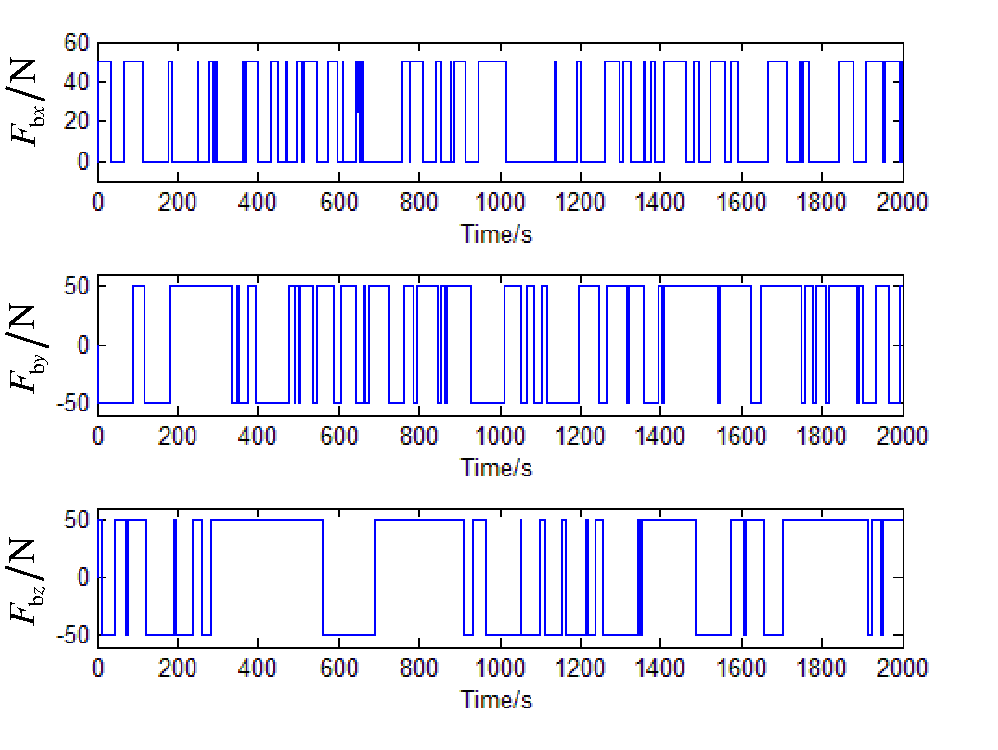
\includegraphics[width=0.7\textwidth]{Chap4/fig26.pdf}
%	\caption{GBN Signal Used to Excite the System}\label{fig4.26}
%\end{figure} 
%\begin{figure}[th]
%	\centering
%	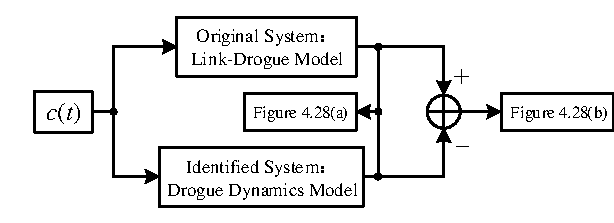
\includegraphics[width=0.7\textwidth]{Chap4/fig27.pdf}
%	\caption{Verification Simulation Framework for Identification Results}\label{fig4.27}
%\end{figure} 
%\begin{figure}[th]
%	\centering
%	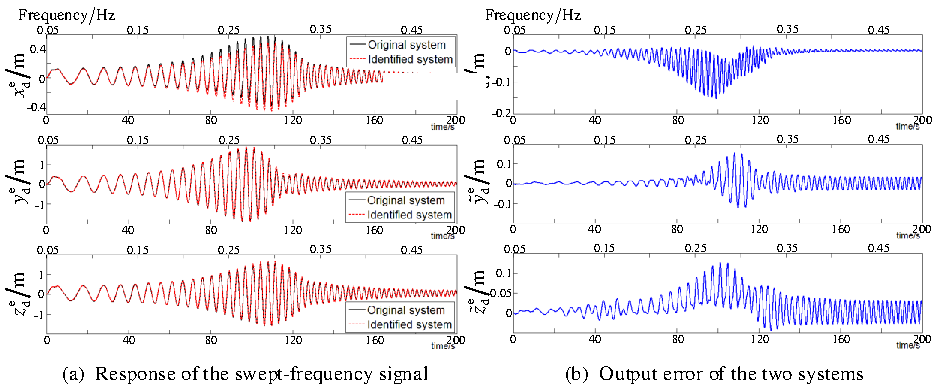
\includegraphics[width=0.7\textwidth]{Chap4/fig28.pdf}
%	\caption{Effectiveness of System Identification}\label{fig4.28}
%\end{figure} 
%From Fig. \ref{fig4.28} (b), it can be observed that the system's tracking error is minimal in the low-frequency range below 0.2 Hz, increases in the mid-frequency range between 0.2 Hz and 0.35 Hz, and remains relatively small in the high-frequency range above 0.35 Hz. The outputs $y_{\rm{d}}^{\rm{e}}$ and $z_{\rm{d}}^{\rm{e}}$ from both models are very close to each other, while the performance of $x_{\rm{d}}^{\rm{e}}$ is relatively poorer. This is mainly due to the higher nonlinearity exhibited by the link-connected hose-drogue model when subjected to ${\bf{F}_{{\rm{b}}x - }}$, which occurs rarely in actual docking scenarios. Therefore, the identified drogue dynamics model effectively captures the drogue dynamics of the link-connected hose-drogue model.
%
%It should be noted that the above model was derived under the assumption of no crosswind or minimal crosswind. In the presence of a crosswind, the $y$-axis becomes coupled with the other axes, meaning that all elements within Eq. (\ref{eq4.132}) would be non-zero. However, the drogue dynamics model can still be obtained using the identification method described above. Since the refueling process allows for adjustments in the direction of the aircraft's velocity to minimize the impact of crosswind disturbances, this chapter primarily focuses on the model under the assumption of no crosswind.
%
%\subsection{Dynamic Model of Drogue with HDU and Quantitative Analysis}
%
%Using the system identification steps described in Sections 4.5.2-4.5.4, the simplified drogue dynamics model for the link-connected hose-drogue system with HDU was obtained. The identification results are presented in Table \ref{tab4.5}. The controller choices are as shown in Section 4.3.3: for the first type of HDU controller (\ref{eq4.123}), the parameter is set as $k = 0.5$, and for the second type of HDU controller (\ref{eq4.124}), the parameters are chosen as $k = 0.5$ and ${k_d} = 500$. In the table, the fitness metric is used to represent the identification performance, defined as $1 - {{\left\| {\bm{y} - \bm{\hat y}} \right\|} /{\left\| {\bm{y} - \bm{\bar y}} \right\|}}$, where $\bm{y},\bm{\hat y}$ and $\bm{\bar y}$ represent the output of the original model, the the output of the identification model, and the mean of the output of the original model, respectively.
%
%Unlike the drogue dynamics without considering HDU (Eq. (\ref{eq4.131})), the identification in Table \ref{tab4.5} utilizes a fourth-order model. The reason behind this choice is that the drogue dynamics without HDU are second-order, while the HDU itself introduces an additional second-order dynamics. Hence, a fourth-order model is employed to identify the link-connected hose-drogue system with HDU. Moreover, judging from the fitness values in the identification results, the fourth-order model also performs better than the second-order model. From Table \ref{tab4.5}, the following conclusions regarding the drogue dynamics can be drawn:
%
%1) The transition process under the control of the second-class controller exhibits significantly better performance compared with the first-class controller. This is due to the fact that, in comparison to the first-class controller, the poles of the drogue dynamic model under the second-class controller are far from the imaginary axis.
%
%2) From the fitness values in Table \ref{tab4.5}, it is evident that the identification results of the drogue dynamics under the control of the first-class controller are inferior to those under the second-class controller. This is due to the higher level of nonlinearity exhibited by the drogue dynamics under the first-class controller, which is also evident from Figs. \ref{fig4.25} (a3) and (a4). Therefore, if a more accurate drogue dynamic model is desired, employing the second-class controller for HDU control is more appropriate.
%
%% Table generated by Excel2LaTeX from sheet 'Sheet1'
%\begin{table}[htbp]
%	\centering
%	\caption{Drogue Dynamic Model Considering HDU (Controller Parameter $k=0.5$)}
%	  \begin{tabular}{|c|r|r|r|}
%	 \hline \diagbox{Controller}{Results} & \multicolumn{2}{c|}{Transfer function} & \multicolumn{1}{l|}{Fitness} \\ \hline
%	  \multirow{5}[0]{*}{First-Class HDU Controller} &   ${G_{xx}}\left( s \right)$    &    $\frac{{0.012{s^2} + 0.012s + 0.052}}{{{s^4} + 2.15{s^3} + 9.17{s^2} + 7.54s + {\rm{18}}{\rm{.21}}}}$   &$89.4\% $  \\ \cline{2-4}
%			&    ${G_{xz}}\left( s \right)$   &   $\frac{{0.0010{s^2} + 0.0057s + 0.046}}{{{s^4} + 13.49{s^3} + 19.29{s^2} + 35.69s + {\rm{29}}{\rm{.50}}}}$    &$70.9\% $  \\ \cline{2-4}
%			&    ${G_{yy}}\left( s \right)$   &   $\frac{{0.026{s^2} + 0.0034s + 0.42}}{{{s^4} + 0.39{s^3} + 24.02{s^2} + 5.76s + {\rm{49}}{\rm{.66}}}}$    &  $99.5\% $\\ \cline{2-4}
%			&    ${G_{zx}}\left( s \right)$   &   $\frac{{0.0026{s^2} + 0.010s + 0.032}}{{{s^4} + 1.76{s^3} + 11.03{s^2} + 7.04s + {\rm{20}}{\rm{.01}}}}$    & $85.1\% $ \\ \cline{2-4}
%			&    ${G_{zz}}\left( s \right)$   &   $\frac{{0.027{s^2} + 0.0011s + 0.38}}{{{s^4} + 0.56{s^3} + 24.22{s^2} + 7.06s + {\rm{53}}{\rm{.95}}}}$    & $94.5\% $ \\ \hline
%	  \multirow{5}[0]{*}{Second-Class HDU Controller} &   ${G_{xx}}\left( s \right)$   &   $\frac{{0.0090{s^2} + 0.011s + 0.021}}{{{s^4} + 4.01{s^3} + 6.61{s^2} + 10.48s + {\rm{7}}{\rm{.38}}}}$    & $98.3\% $ \\ \cline{2-4}
%			&    ${G_{xz}}\left( s \right)$   &    $\frac{{0.0048{s^2} + 0.019s + 0.0085}}{{{s^4} + 3.29{s^3} + 5.77{s^2} + 8.44s + {\rm{5}}{\rm{.80}}}}$   & $98.5\% $ \\ \cline{2-4}
%			&    ${G_{yy}}\left( s \right)$   &   $\frac{{0.026{s^2} + 0.0033s + 0.42}}{{{s^4} + 0.40{s^3} + 24.01{s^2} + 5.75s + {\rm{49}}{\rm{.62}}}}$    & $99.6\% $ \\ \cline{2-4}
%			&    ${G_{zx}}\left( s \right)$   &   $\frac{{0.0051{s^2} + 0.0091s + 0.0051}}{{{s^4} + 1.96{s^3} + 4.32{s^2} + 4.71s + {\rm{3}}{\rm{.14}}}}$    & $93.2\% $ \\ \cline{2-4}
%			&    ${G_{zz}}\left( s \right)$   &    $\frac{{0.027{s^2} + 0.0046s + 0.39}}{{{s^4} + 0.61{s^3} + 24.05{s^2} + 7.71s + {\rm{55}}{\rm{.76}}}}$   & $89.4\% $ \\ \hline
%	  \end{tabular}%
%	\label{tab4.6}%
%\end{table}%
%  
%3) By comparing Table \ref{tab4.5} with the transfer function in Eq. (\ref{eq4.131}), it can be observed that the presence or absence of HDU significantly affects the drogue dynamics. Next, the impact of HDU on the drogue dynamics will be further analyzed by comparing their Direct Current Gain (DC Gain) of the transfer functions \cite{franklin_feedback_2015}. Taking the coefficients of the two classes of controllers as $k = \left\{ {0.3,0.5,1,3} \right\}$, the results are shown in Table \ref{tab4.6}.
%
%Based on Table \ref{tab4.6}, the following conclusions can be drawn regarding the drogue dynamics.
%
%1) The gains of the drogue dynamics models under both types of controllers are similar. In other words, the second type of controller only affects the transient behavior, while the steady-state values of both types are the same.
%
%2) The primary factor influencing the DC gain is the controller coefficient $k$. The smaller the value of $k$, the more pronounced the impact, especially on ${G_{xx}}\left( s \right)$ and ${G_{zx}}\left( s \right)$. In this case, the decoupling between the $x$-channel and  $z$-channel is better, indicated by the fact that the gains of ${G_{zx}}\left( s \right)$ and ${G_{xz}}\left( s \right)$ are much smaller than those of ${G_{xx}}\left( s \right)$ and ${G_{zz}}\left( s \right)$. Conversely, as $k$ increases, coupling becomes more pronounced. For instance, when $k = 3$, the DC gain of the drogue dynamics model with HDU is already approaching that of the model without HDU.
%
%3) The impact of HDU on the DC gain of the y-axis is not significant.
%
%In summary, when designing HDU controllers with the aim of mitigating the hose whipping phenomenon, a larger value of $k$ should be selected. This choice would require fewer adjustments to achieve regulation and speed up the adjustment process. On the other hand, if the intention is to decouple the dynamics of the drogue, facilitating controller design, a smaller value of $k$ should be chosen. Therefore, the selection of $k$ should balance between these two aspects.
%
%% Table generated by Excel2LaTeX from sheet 'Sheet1'
%\begin{table}[htbp]
%	\centering
%	\caption{DC gain of drogue dynamic model model with or without HDU (order of magnitude is $10^{-4}$)}
%	  \begin{tabular}{|c|c|c|c|c|c|c|}
%	  \hline \multirow{2}[0]{*}{\diagbox{Transfer function}{Drogue model type}} & \multicolumn{5}{c|}{Considering HDU}             & \multirow{2}[0]{*}{Without considering HDU} \\ \cline{2-6}
%			& HDU Controller & $k = 0.3$     & $k = 0.5$     & $k = 1$     & $k = 3$     &  \\ \hline
%			\multirow{2}[0]{*}{ ${G_{xx}}\left( s \right)$}     & First-Class   & 41.6  & 28.69 & 18.96 & 12.59 &  \multirow{2}[0]{*}{8.15} \\ \cline{2-6}
%			& Second-Class   & 42.04 & 28.98 & 19.15 & 12.64 &  \\ \hline
%			\multirow{2}[0]{*}{ ${G_{xz}}\left( s \right)$}     & First-Class   & 8.08  & 14.48 & 20.07 & 23.56 & \multirow{2}[0]{*}{22.94} \\ \cline{2-6}
%			& Second-Class   & 7.42  & 14.56 & 19.93 & 23.52 &  \\ \hline
%			\multirow{2}[0]{*}{ ${G_{yy}}\left( s \right)$}     & First-Class   & 84.65 & 84.58 & 84.72 & 84.75 & \multirow{2}[0]{*}{82.29} \\ \cline{2-6}
%			& Second-Class   & 84.65 & 84.68 & 84.73 & 84.75 &  \\ \hline
%			\multirow{2}[0]{*}{ ${G_{zx}}\left( s \right)$}     & First-Class   & 11.81 & 15.98 & 19.78 & 21.77 & \multirow{2}[0]{*}{8.15} \\ \cline{2-6}
%			& Second-Class   & 11.48 & 16.31 & 19.54 & 21.78 &  \\ \hline
%			\multirow{2}[0]{*}{ ${G_{zz}}\left( s \right)$}     & First-Class   & 72.42 & 69.99 & 68.22 & 67.13 & \multirow{2}[0]{*}{66.32} \\ \cline{2-6}
%			& Second-Class   & 72.02 & 69.76 & 68.2  & 67.08 &  \\ \hline
%	  \end{tabular}%
%	\label{tab4.7}%
%\end{table}%
%  
%If establishing a simulation environment similar to the one in Section 4.3.4 and replaceing the link-connected hose-drogue model with the drogue dynamic model with HDU (as shown in Table \ref{tab4.5}), simulation results as depicted in Fig. \ref{fig4.29} can be obtained. To visually display the differences in drogue dynamics with and without HDU during the docking process, as well as the differences in drogue dynamics under different controllers, a video have also been recorded. Readers can refer to Ref. \cite{noauthor_drogue_nodate-1} for the video, and a screenshot from the video is shown in Fig. \ref{fig4.30}. In the screenshot, View 1 represents the pilot's perspective, and View 2 provides a lateral view. The HDU used in the screenshot employs the first type of controller, which is common in current HDU designs. This choice accurately reflects the flight conditions in the experiment. To compare with the results from Ref. \cite{dibley_autonomous_2007}, the units for position are given in feet.
%\begin{figure}[th]
%	\centering
%	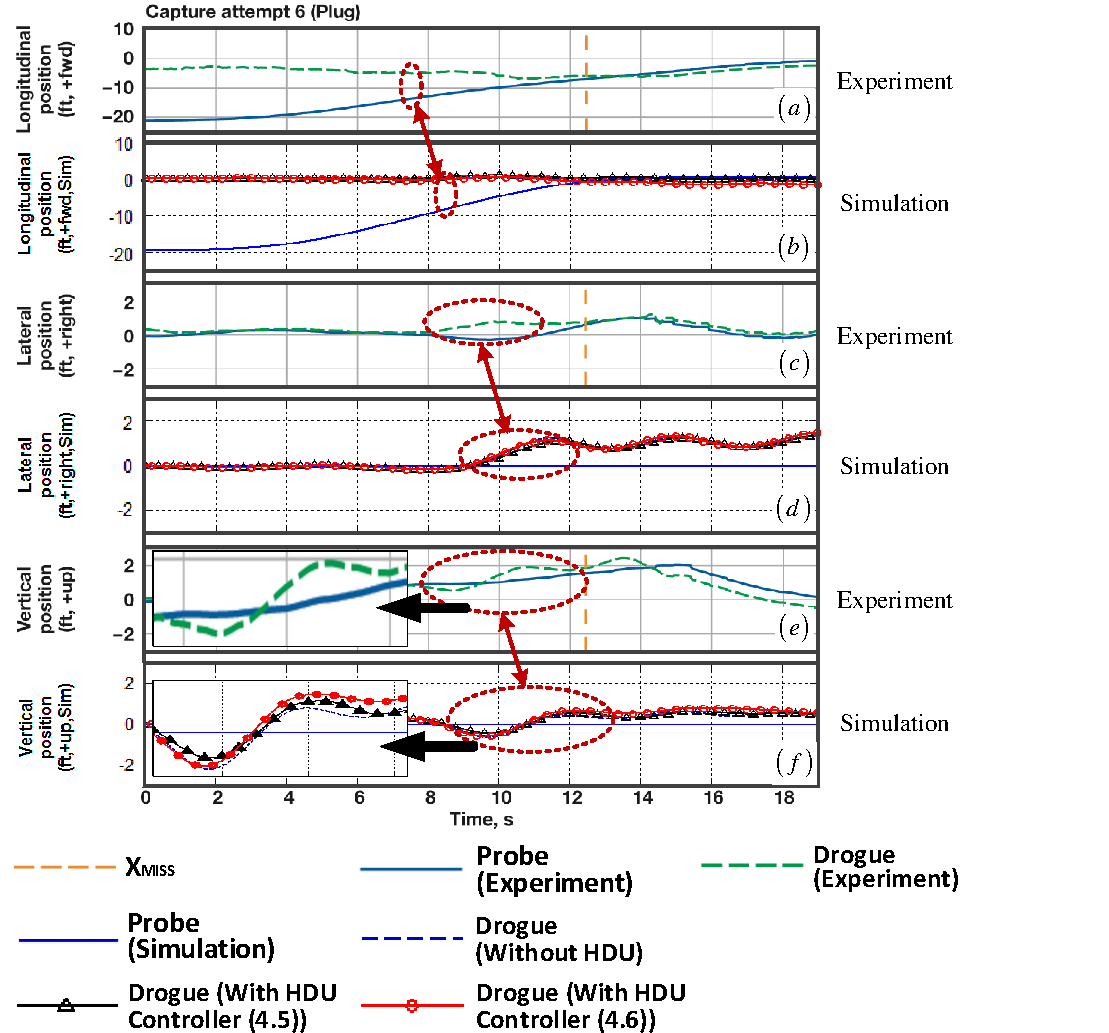
\includegraphics[width=0.7\textwidth]{Chap4/fig29.pdf}
%	\caption{Comparison of Drogue Dynamics during the Docking Process}\label{fig4.29}
%\end{figure} 
%Based on Fig. \ref{fig4.29}, the HDU has a slight influence on the drogue dynamics. However, during the docking process, even a small error of a few centimeters can lead to docking failure. Therefore, this influence remains significant. The two subplots Fig. \ref{fig4.29} (e) and (f) illustrate the differences in drogue dynamics in the vertical direction during docking, which is in accordance with the issue highlighted in the conclusions of Section 4.3.
%Additionally, from Fig. \ref{fig4.30}, it is even more evident that compared with the scenario without HDU, the vertical descent of the drogue with HDU is significantly reduced. In other words, the drogue dynamics considering the HDU model closely resemble the drogue dynamics observed in experiments.
%
%On the other hand, from Fig. \ref{fig4.29}, it is evident that the drogue dynamics under the control of the second type of controller differ from those without HDU and those under the control of the first type of controller. Although the swing amplitude of the drogue increases under the second type of controller, its adjustment speed is faster, which is more conducive to suppressing the hose whipping phenomenon. Furthermore, it can lead to a more accurate linearization of the model for the link-connected hose-drogue system with HDU. Therefore, it is still recommended to use the second type of controller for future HDU controller design.
%\begin{figure}[th]
%	\centering
%	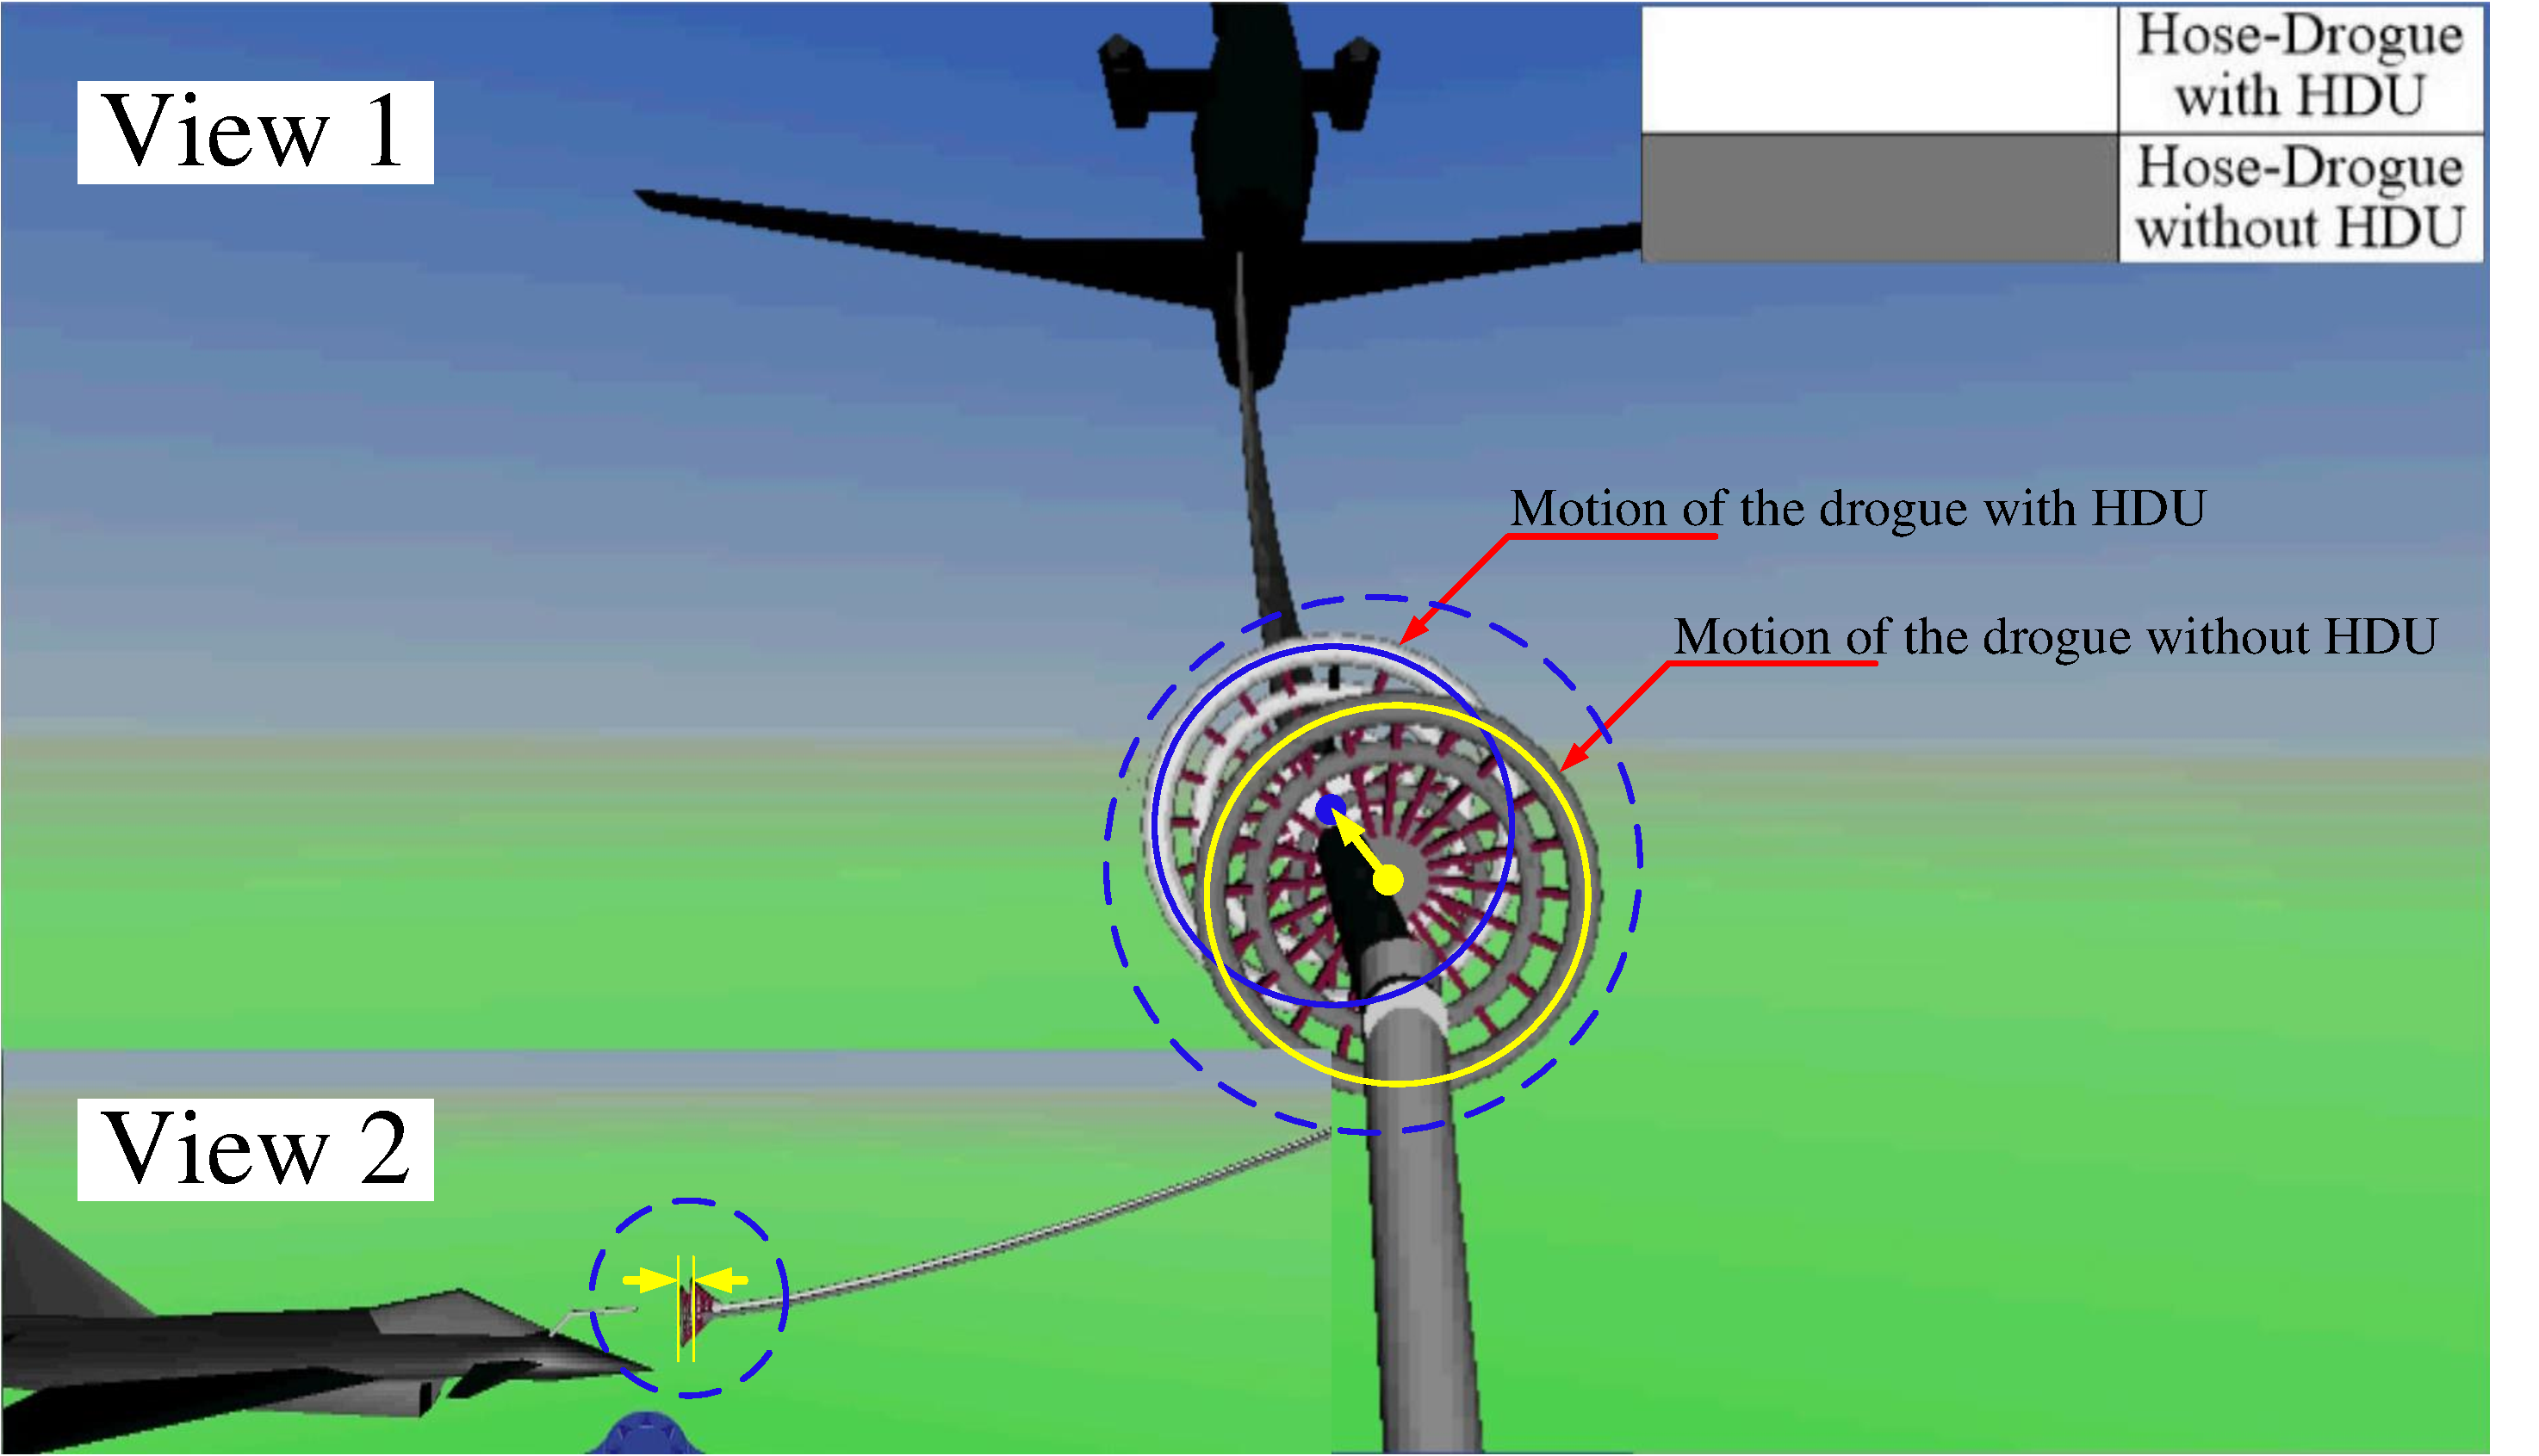
\includegraphics[width=0.7\textwidth]{Chap4/fig30.pdf}
%	\caption{Screenshot of the Simulation Video at Maximum Drogue Subsidence}\label{fig4.30}
%\end{figure} 